% vim:spelllang=en_us:spell
% Author: Marek Filip 2022

%==============================================================================
% tento soubor pouzijte jako zaklad
% this file should be used as a base for the thesis
% Autoři / Authors: 2008 Michal Bidlo, 2019 Jaroslav Dytrych
% Kontakt pro dotazy a připomínky: sablona@fit.vutbr.cz
% Contact for questions and comments: sablona@fit.vutbr.cz
%==============================================================================
% kodovani: UTF-8 (zmena prikazem iconv, recode nebo cstocs)
% encoding: UTF-8 (you can change it by command iconv, recode or cstocs)
%------------------------------------------------------------------------------
% zpracování / processing: make, make pdf, make clean
%==============================================================================
%\documentclass[]{fitthesis} % bez zadání - pro začátek práce, aby nebyl problém s překladem
%\documentclass[english]{fitthesis} % without assignment - for the work start to avoid compilation problem
%\documentclass[zadani]{fitthesis} % odevzdani do wisu a/nebo tisk s barevnými odkazy - odkazy jsou barevné
\documentclass[english,zadani,odsaz]{fitthesis} % for submission to the IS FIT and/or print with color links - links are color
%\documentclass[zadani,print]{fitthesis} % pro černobílý tisk - odkazy jsou černé
%\documentclass[english,zadani,print]{fitthesis} % for the black and white print - links are black
%\documentclass[zadani,cprint]{fitthesis} % pro barevný tisk - odkazy jsou černé, znak VUT barevný
%\documentclass[english,zadani,cprint]{fitthesis} % for the print - links are black, logo is color
% * Je-li práce psaná v anglickém jazyce, je zapotřebí u třídy použít
%   parametr english následovně:
%   If thesis is written in English, it is necessary to use
%   parameter english as follows:
%      \documentclass[english]{fitthesis}
% * Je-li práce psaná ve slovenském jazyce, je zapotřebí u třídy použít
%   parametr slovak následovně:
%   If the work is written in the Slovak language, it is necessary
%   to use parameter slovak as follows:
%      \documentclass[slovak]{fitthesis}
% * Je-li práce psaná v anglickém jazyce se slovenským abstraktem apod.,
%   je zapotřebí u třídy použít parametry english a enslovak následovně:
%   If the work is written in English with the Slovak abstract, etc.,
%   it is necessary to use parameters english and enslovak as follows:
%      \documentclass[english,enslovak]{fitthesis}

% Základní balíčky jsou dole v souboru šablony fitthesis.cls
% Basic packages are at the bottom of template file fitthesis.cls
% zde můžeme vložit vlastní balíčky / you can place own packages here

% Kompilace po částech (rychlejší, ale v náhledu nemusí být vše aktuální)
% Compilation piecewise (faster, but not all parts in preview will be up-to-date)
% \usepackage{subfiles}

% Nastavení cesty k obrázkům
% Setting of a path to the pictures
\graphicspath{{figures/}{./figures/}}
%\graphicspath{{figures/}{../figures/}}

%---rm---------------
\renewcommand{\rmdefault}{lmr}%zavede Latin Modern Roman jako rm / set Latin Modern Roman as rm
%---sf---------------
\renewcommand{\sfdefault}{qhv}%zavede TeX Gyre Heros jako sf
%---tt------------
\renewcommand{\ttdefault}{lmtt}% zavede Latin Modern tt jako tt

% vypne funkci šablony, která automaticky nahrazuje uvozovky,
% aby nebyly prováděny nevhodné náhrady v popisech API apod.
% disables function of the template which replaces quotation marks
% to avoid unnecessary replacements in the API descriptions etc.
\csdoublequotesoff


\usepackage{url}


% =======================================================================
% balíček "hyperref" vytváří klikací odkazy v pdf, pokud tedy použijeme pdflatex
% problém je, že balíček hyperref musí být uveden jako poslední, takže nemůže
% být v šabloně
% "hyperref" package create clickable links in pdf if you are using pdflatex.
% Problem is that this package have to be introduced as the last one so it
% can not be placed in the template file.
\ifWis
\ifx\pdfoutput\undefined % nejedeme pod pdflatexem / we are not using pdflatex
\else
  \usepackage{color}
  \usepackage[unicode,colorlinks,hyperindex,plainpages=false,pdftex]{hyperref}
  \definecolor{hrcolor-ref}{RGB}{223,52,30}
  \definecolor{hrcolor-cite}{HTML}{2F8F00}
  \definecolor{hrcolor-urls}{HTML}{092EAB}
  \hypersetup{
	linkcolor=hrcolor-ref,
	citecolor=hrcolor-cite,
	filecolor=magenta,
	urlcolor=hrcolor-urls
  }
  \def\pdfBorderAttrs{/Border [0 0 0] }  % bez okrajů kolem odkazů / without margins around links
  \pdfcompresslevel=9
\fi
\else % pro tisk budou odkazy, na které se dá klikat, černé / for the print clickable links will be black
\ifx\pdfoutput\undefined % nejedeme pod pdflatexem / we are not using pdflatex
\else
  \usepackage{color}
  \usepackage[unicode,colorlinks,hyperindex,plainpages=false,pdftex,urlcolor=black,linkcolor=black,citecolor=black]{hyperref}
  \definecolor{links}{rgb}{0,0,0}
  \definecolor{anchors}{rgb}{0,0,0}
  \def\AnchorColor{anchors}
  \def\LinkColor{links}
  \def\pdfBorderAttrs{/Border [0 0 0] } % bez okrajů kolem odkazů / without margins around links
  \pdfcompresslevel=9
\fi
\fi
% Řešení problému, kdy klikací odkazy na obrázky vedou za obrázek
% This solves the problems with links which leads after the picture
\usepackage[all]{hypcap}

% Mou definovovane package
\usepackage{caption}
\usepackage{subcaption}
\usepackage{minted}
\usepackage{verbatim}
\usepackage{pmboxdraw}

% Informace o práci/projektu / Information about the thesis
%---------------------------------------------------------------------------
\projectinfo{
  %Prace / Thesis
  project={BP},            %typ práce BP/SP/DP/DR  / thesis type (SP = term project)
  year={2022},             % rok odevzdání / year of submission
  date=\today,             % datum odevzdání / submission date
  %Nazev prace / thesis title
  title.cs={Adaptivní obchodní strategie pro kryptoměny},  % název práce v češtině či slovenštině (dle zadání) / thesis title in czech language (according to assignment)
  title.en={Adaptive Trading Strategies for Cryptocurrencies}, % název práce v angličtině / thesis title in english
  %title.length={14.5cm}, % nastavení délky bloku s titulkem pro úpravu zalomení řádku (lze definovat zde nebo níže) / setting the length of a block with a thesis title for adjusting a line break (can be defined here or below)
  %sectitle.length={14.5cm}, % nastavení délky bloku s druhým titulkem pro úpravu zalomení řádku (lze definovat zde nebo níže) / setting the length of a block with a second thesis title for adjusting a line break (can be defined here or below)
  %dectitle.length={14.5cm}, % nastavení délky bloku s titulkem nad prohlášením pro úpravu zalomení řádku (lze definovat zde nebo níže) / setting the length of a block with a thesis title above declaration for adjusting a line break (can be defined here or below)
  %Autor / Author
  author.name={Marek},   % jméno autora / author name
  author.surname={Filip},   % příjmení autora / author surname
  %author.title.p={Bc.}, % titul před jménem (nepovinné) / title before the name (optional)
  %author.title.a={Ph.D.}, % titul za jménem (nepovinné) / title after the name (optional)
  %Ustav / Department
  department={UITS}, % doplňte příslušnou zkratku dle ústavu na zadání: UPSY/UIFS/UITS/UPGM / fill in appropriate abbreviation of the department according to assignment: UPSY/UIFS/UITS/UPGM
  % Školitel / supervisor
  supervisor.name={Ivan},   % jméno školitele / supervisor name
  supervisor.surname={Homoliak},   % příjmení školitele / supervisor surname
  supervisor.title.p={Ing.},   %titul před jménem (nepovinné) / title before the name (optional)
  supervisor.title.a={Ph.D.},    %titul za jménem (nepovinné) / title after the name (optional)
  % Klíčová slova / keywords
  keywords.cs={Kryptoměna, obchodování, investování, obchodní strategie, simulace, adaptivní obchodní strategie, simulační nástroj, backtester, backtesting, Bitcoin risk metric, cryptocurrency data API, testování, testování s historickými daty}, % klíčová slova v českém či slovenském jazyce / keywords in czech or slovak language
  keywords.en={Cryptocurrency, trading, investing, trading strategies, simulation, adaptive trading strategy, simulation tool, backtester, backtesting, Bitcoin risk metric, cryptocurrency data API}, % klíčová slova v anglickém jazyce / keywords in english
  %keywords.en={Here, individual keywords separated by commas will be written in English.},
  % Abstrakt / Abstract
    abstract.cs={Obchodní strategie pro kryptoměny bývají založeny buď na padajícím či stoupajícím trhu. Kámen úrazu nastává, když jsou aplikovány na špatný trend v tak nestabilním trhu, jako je ten s kryptoměny. Tato práce se zabývá možností adaptivních obchodních strategií, které se dokáží přizpůsobit na klesajicí a stoupající trendy v kryptoměnovém trhu. Analyzováním ceny Bitcoinu a vytvořením metriky risku, kde se díváme na extrémy vytvořené funkce, můžeme dojít k řešení návrhu adaptivních strategií. Zkoumají se jak dlouhodobé, tak krátkodobé možnosti investování. K vyhodnocování strategií a vykreslování časových řad je vytvořen rozšířitelný program pro testování historických dat. Výsledky jsou porovnány s tradičními přistupy, jako je HODL a rebalancování, přičemž bylo zjištěno, že při použití správných kritérií se mohou risky vice než ztrojnásobit. Práce nabízí investorům nové způsoby zisků a zároveň dává čtenárům možnost náhlednout do tvorby (adaptivních) strategií a jejich zpětného testování v kódu. Předpokládá se, že výsledky práce budou využívány automatizovanými obchodními systémy.}, % abstrakt v českém či slovenském jazyce / abstract in czech or slovak language
  abstract.en={Cryptocurrency trading strategies are based on either rising or falling markets, however, they fail when applied to the wrong trend in a volatile market.
This thesis explores the idea of cryptocurrency trading in rising and falling markets with adaptive strategies that can adjust to current market trends in order to maximize effectiveness.
The problem is solved by analyzing the Bitcoin price, creating risk metric and focusing on the function's extrema. Both long-term and short-term options are explored.
An extensible backtester program is created to evaluate the strategies and plot the time series.
The results are compared to traditional approaches like HODL and rebalance, the profits can multiply more than three times using the right criteria.
The thesis offers new ways of gaining profit to cryptocurrency investors, as well as giving readers insight into creating (adaptive) trading strategies and backtesting them in code. The output of the thesis is expected to be used by automated trading systems.

}, % abstrakt v anglickém jazyce / abstract in english
  % Prohlášení (u anglicky psané práce anglicky, u slovensky psané práce slovensky) / Declaration (for thesis in english should be in english)
  %declaration={Prohlašuji, že jsem tuto bakalářskou práci vypracoval samostatně pod vedením pana X...
%Další informace mi poskytli...
%Uvedl jsem všechny literární prameny, publikace a další zdroje, ze kterých jsem čerpal.},
  declaration={I hereby declare that this Bachelor's thesis was prepared as an original work by the author under the supervision of Ing. Ivan Homoliak, Ph.D.
 I have listed all the literary sources, publications and other sources, which were used during the preparation of this thesis.},
  % Poděkování (nepovinné, nejlépe v jazyce práce) / Acknowledgement (optional, ideally in the language of the thesis)
  %acknowledgment={V této sekci je možno uvést poděkování vedoucímu práce a těm, kteří poskytli odbornou pomoc
%(externí zadavatel, konzultant apod.).},
  acknowledgment={I would like to acknowledge and give my thanks to my supervisor Ing. Ivan Homoliak, Ph.D., for leading me in the right direction. My warmest thanks also go to my work colleague and mentor, Hubert Stefanski. You have gone above and beyond to give me practical advice and share your experiences. Lastly, I want to thank my friends and family for their continuous support and belief they have in me.},
  % Rozšířený abstrakt (cca 3 normostrany) - lze definovat zde nebo níže / Extended abstract (approximately 3 standard pages) - can be defined here or below
  extendedabstract={Trh s kryptoměnami je pro lidi, kteří chtěji při jejich obchodování vydělat, velmi lukrativní a neustále se přichází s novými metodami, jak na to. Mnoho
obchodních strategií pro kryptoměny jsou veřejně k dispozici, ale žádná taková strategie nepřežije jak rostoucí
(býčí) i klesající (medvědí) trh zároveň. Proto jsou potřeba adaptivní strategie, které se dokáží přizpůsobit oběma obdobím, zachováním ceny pří klesajícím trhu a tvořením zisku při soupajícím.

Tato práce se zabývá myšlenkou adaptivních obchodních strategií.
Myšlenka práce představena na vysoké úrovni je následující. Nejprve je třeba najít způsob, jak předpovědět, zda trh půjde nahoru, nebo dolů. Poté využijeme optimální stratege, které budou založeny na zjištěné pravděpodobnostní metrice.
Pro řešení výše nastíněných problémů jsou prozkoumámy současné strategie, které
se používají pro obchodování s kryptoměnami, simulační nástroje, které jsou dnes k dispozici a jsou analyzovány historická data s cílem najít určité zákonitosti. Ohlédnutí se na současný stav adaptivních obchodních strategií je rovněž nezbytné.

Cíl práce byl dosažen a demonstrován několika způsoby se zaměřením na dlouhodobé i krátkodobé datové rozsahy. Přitom byl vytvořen rozšiřitelný program pro zpětné testování, který je dostatečně obecný, aby podporoval implementaci dlouhodobých i krátkodobých strategií.

Co se týka formální specifikace práce. Existující obchodní strategie byly studovány a dosažené výsledky analyzovány a jejich předpoklady shrnuty. Existující simulační nástroje byly popsány. Byla analyzována data o obchodování s kryptoměnami a shrnuty zájímavé události ovlivňující trh. Například, jak tweety Elona Muska, státní regulace a zájem médií mohou dramaticky ovlivnit chování kryptoměnového trhu. Adaptivní obchodní strategie byly navrženy, implementovány ve formě backtester programu a vyhodnoceny oproti tradičním přístupům. V průběhu práce byla použita jak 5minutová OHLCV, tak 1denní OHLCV data. Na závěr byla popsána další vylepšení a omezení praktického nasazení.

Uvedu zde výčet těch zajímavějších strategií a výsledků. Nejprve jsme navrhli a předvedli několik adaptivních strategií. Jednou z nich byla metrika rizika, která nám říká, jak nebezpečné je v daném okamžiku investovat na trhu. Bylo ukázáno, jak lze takové strategie vylepšit optimalizovací pro klesající výnosy. Bylo také ukázáno, jak lze k dalšímu vylepšení strategie využít korelaci s nějakým ukazatelem. Strojové učení pro využití na finančním trhu bylo také krátce prozkoumáno s méně zajímavými výsledky než byly ostatní navržené strategie.

Již zmíněná metrika rizika byla použita jakožto vstupní parametr pro druhou část strategie, vyhodnocovací algoritmus. Tímto směrem bylo zváženo několik možností. Dva hlavní vyhodnocovací větve byly vybrány. První větev se zaměřuje na výměnu mincí na stablecoiny při prodeju a opačným směrem při nákupu. Druhá větev se zaměřuje na investiční strategii průměrování nákladů (DCA), která je užitečným nástrojem mnoha investorů. Pro první větev se ukázalo jako klíčové nalezení lokálních extrémů na rizikové funkci. DCA se blíže zaměřila na to, jak může upravovat své investice dle metriky risku. Se skvělými výsledky bylo nalezeno~řešení založené na Fibonacciho posloupnosti.

S připravenou adaptivní strategií a vyhodnocovací strategií bylo zahájeno testování různých kombinací výše uvedených optimalizací. Byly pozorovány některé oblíbenější trendy, ale výsledky byly někdy příliš rozporuplné, než aby bylo možné učinit jednoznačné závěry. V této fázi byly strategie porovnány se strategiemi HODL, a periodickými strategiemi DCA. Navržené strategie poměrně konzistentně překonávaly tradiční přístupy a v určitých případech vykazovaly velmi dobré výsledky.

V dalším kroku byly strategie podrobeny testu proti dvěma portfoliím obsahujícím více mincí. Portfolio s Bitcoinem a Ethereem si vedlo srovnatelně dobře jako předchozí výsledky a snadno překonalo rebalancování, další tradiční přístup. Druhé portfolio, které obsahovalo 18 různých mincí, vykazovalo horší výsledky. To ukázalo, že při pokusech o investování s různorodými portfolii, jako bylo toto, je třeba provést rozsáhlejší průzkum pro dosažení optimálních výsledků.

Nakonec byly zkoumány možnosti krátkodobého obchodování. Dosud jsme hovořili pouze o dlouhodobém obchodování s frekvencí dat 1 den. Pro účely krátkodobé simulace byla použita 5minutová data OHLCV. K předvídání úrovní podpory a odporu byl použit klouzavý průměr 6 hodin. Strategie byla testována proti několika různým datovým rozsahům, klesajícímu trendu, rostoucímu trendu a měnícímu se trendu. Výsledky strategií byly přinejlepším sporné, v některých úsecích si vedly dobře, v jiných naopak nedostatečně. Bylo usouzeno, že pro spolehlivejší používání strategií je zapotřebí podrobnějšího výzkumu.

Během práce jsem se velmi podrobně naučil o ekonomice obchodování na trhu a o kryptoměnách obecně. Pochopil jsem, jak vytvořit program pro historické testování dat a jak by měla být realizována obchodní strategie.

Co se týče mých plánů do budoucna, plánuji nadále pracovat na samotném programu. Existuje několik vylepšení, která by se mohla uplatnit, například optimalizace výpočetního času nebo vytvoření webové uživatelské rozhraní. Existuje také mnoho strategií, které stojí za to prozkoumat. Například pokus o generování zisku z obchodování se stablecoiny při jejich držení, podrobnější využití strojového učení a mnoho dalších. K zajímavým objevům může vést i pokročilejší analýza zisku, například Sharpeho poměr a vizualizace zisku a ztrát při individuálních objednávkách nákupu a prodeje. Mezi mé další plány patří vytvoření automatického obchodního systému, který by používal strategie zpětně otestované programem této práce.
},
  %extabstract.odd={true}, % Začít rozšířený abstrakt na liché stránce? / Should extended abstract start on the odd page?
  %faculty={FIT}, % FIT/FEKT/FSI/FA/FCH/FP/FAST/FAVU/USI/DEF
  faculty.cs={Fakulta informačních technologií}, % Fakulta v češtině - pro využití této položky výše zvolte fakultu DEF / Faculty in Czech - for use of this entry select DEF above
  faculty.en={Faculty of Information Technology}, % Fakulta v angličtině - pro využití této položky výše zvolte fakultu DEF / Faculty in English - for use of this entry select DEF above
  department.cs={Ústav inteligentních systémů}, % Ústav v češtině - pro využití této položky výše zvolte ústav DEF nebo jej zakomentujte / Department in Czech - for use of this entry select DEF above or comment it out
  department.en={Department of Intelligent Systems} % Ústav v angličtině - pro využití této položky výše zvolte ústav DEF nebo jej zakomentujte / Department in English - for use of this entry select DEF above or comment it out
}

% Rozšířený abstrakt (cca 3 normostrany) - lze definovat zde nebo výše / Extended abstract (approximately 3 standard pages) - can be defined here or above
%\extendedabstract{Do tohoto odstavce bude zapsán výtah (abstrakt) práce v českém (slovenském) jazyce.}
% Začít rozšířený abstrakt na liché stránce? / Should extended abstract start on the odd page?
%\extabstractodd{true}

% nastavení délky bloku s titulkem pro úpravu zalomení řádku - lze definovat zde nebo výše / setting the length of a block with a thesis title for adjusting a line break - can be defined here or above
%\titlelength{14.5cm}
% nastavení délky bloku s druhým titulkem pro úpravu zalomení řádku - lze definovat zde nebo výše / setting the length of a block with a second thesis title for adjusting a line break - can be defined here or above
%\sectitlelength{14.5cm}
% nastavení délky bloku s titulkem nad prohlášením pro úpravu zalomení řádku - lze definovat zde nebo výše / setting the length of a block with a thesis title above declaration for adjusting a line break - can be defined here or above
%\dectitlelength{14.5cm}

% řeší první/poslední řádek odstavce na předchozí/následující stránce
% solves first/last row of the paragraph on the previous/next page
\clubpenalty=10000
\widowpenalty=10000

% checklist
\newlist{checklist}{itemize}{1}
\setlist[checklist]{label=$\square$}

% Nechcete-li, aby se u oboustranného tisku roztahovaly mezery pro zaplnění stránky, odkomentujte následující řádek / If you do not want enlarged spacing for filling of the pages in case of duplex printing, uncomment the following line
% \raggedbottom

\begin{document}
  % Vysazeni titulnich stran / Typesetting of the title pages
  % ----------------------------------------------
  \maketitle
  % Obsah
  % ----------------------------------------------
  \setlength{\parskip}{0pt}

  {\hypersetup{hidelinks}\tableofcontents}

  % Seznam obrazku a tabulek (pokud prace obsahuje velke mnozstvi obrazku, tak se to hodi)
  % List of figures and list of tables (if the thesis contains a lot of pictures, it is good)
  \ifczech
    \renewcommand\listfigurename{Seznam obrázků}
  \fi
  \ifslovak
    \renewcommand\listfigurename{Zoznam obrázkov}
  \fi
  % {\hypersetup{hidelinks}\listoffigures}

  \ifczech
    \renewcommand\listtablename{Seznam tabulek}
  \fi
  \ifslovak
    \renewcommand\listtablename{Zoznam tabuliek}
  \fi
  % {\hypersetup{hidelinks}\listoftables}

  \ifODSAZ
    \setlength{\parskip}{0.5\bigskipamount}
  \else
    \setlength{\parskip}{0pt}
  \fi

  % vynechani stranky v oboustrannem rezimu
  % Skip the page in the two-sided mode
  \iftwoside
    \cleardoublepage
  \fi

  % Text prace / Thesis text
  % ----------------------------------------------
  % vim:spelllang=en_us:spell
% Author: Marek Filip 2022

\chapter{Introduction}

The cryptocurrency market is very lucrative for people that want to turn a profit in cryptocurrency trading, constantly coming up with new methods of doing so. There are many trading strategies for cryptocurrencies available, but no such strategy survives both rising (bull) and falling (bear) market. That is why there is a need for adaptive strategies that can prosper through both of them. That is why there is a need for adaptive strategies that can adjust and react to the market changes, keeping its value in a bear market and creating profit in bull runs.

I~will explore the idea of the adaptive trading strategies for cryptocurrencies in this thesis. Firstly, we need to find a way how to predict if the market will go up or down. Then we need to apply sufficient trading strategies based on the percentage probability of trends rising or falling. That is the high-level overview of the idea presented in this thesis.

To address the problems outlined above, I~will explore the current trading strategies that are used for trading cryptocurrencies. Research current simulation tools available today and analyze the historic trading data to find some patterns. Looking at current state of adaptive strategies for cryptocurrencies is also necessary.


\subsection*{Organization}

The rest of this work is divided into several chapters.

Chapter~\ref{chapter-background}, gives the reader a sufficient theoretical background that is required to understand the later chapters of the thesis. In Chapter~\ref{chapter-trading-stategies} I~look at the existing trading strategies and analyze their effectiveness. In Chapter~\ref{chapter-simulation-tools} several existing simulation tools are explored and compared. During Chapter~\ref{chapter-data-analysis} the backlog of cryptocurrency trading data provided by the supervisor is analyzed and the important events summarized.

After these chapters, the thesis becomes more oriented towards the project goal of the backtester itself. In Chapter~\ref{chapter-implementation} the design, development and implementation of the backtester itself is detailed. After that, in Chapter~\ref{chapter-experiments} adaptive trading strategies are proposed and tested using the developed backtester, and results are evaluated. Finally, limitations and further improvements of practical deployment are discussed in Chapter~\ref{chapter-limitations-and-improvements}

\chapter{Background}
\label{chapter-background}

To understand the full context of the thesis, the reader should be familiarized with certain concepts and terms that will be used regularly throughout the thesis. This section aims to provide this context.

\subsection*{List of Terms Generally Used in the Thesis and Among Cryptocurrency Investors}
\begin{itemize}
    \item Best strategy: A~strategy that yields the most money -- has the best profit.
    \item Bear market: A~market in which prices are falling, encouraging selling.
    \item Bull market: A~market in which prices are rising, encouraging buying.
    \item Fiat currency: Government-issued money.
    \item Spread: Difference between buy and sell value of an asset.
    \item DCA: dollar-cost averaging.
    \item OHLCV: open, high, low, close, value -- type of candlestick data.
    \item MA: moving average, usually refers to smooth moving average (SMA).
    \item SMA: smooth moving average.
    \item ROI: Return of investment.
    \item FOMO: Fear of missing out.
    \item FUD: Fear, uncertainty, doubt.
    \item API: Application programming interface.
    \item crypto $\Leftrightarrow$ cryptocurrency.
    \item 1d $\Leftrightarrow$ 1 day.
    \item 5m $\Leftrightarrow$ 5 minute.
    \item Sell $\Leftrightarrow$ transfer coins to stablecoins.
\end{itemize}

\section{What Is a Cryptocurrency?}
A~\emph{cryptocurrency} is a digital currency that is secured by cryptography~\cite{investopedia-cryptocurrency}. There are algorithms in place that make it nearly impossible to counterfeit or double-spend the currency. Cryptocurrencies are based on a decentralized networks based on the blockchain (see~\ref{blockchain}) technology. Because of this, the cryptocurrencies are not issued by any central authority (unlike conventional currency). This makes them theoretically immune to government interference or manipulation.

\subsection*{Types of Cryptocurrency}
\emph{Bitcoin} is the original and to this day the most popular and valuable cryptocurrency. It was invented by an anonymous person called \emph{Satoshi Nakamoto} in 2008 via a white paper~\cite{satoshi}. As of 12th January 2022, there are over 18.9 million Bitcoins in circulation with a total market capitalization of around \$810 million~\cite{coinmarketcap}, making it roughly 40\% of the total cryptocurrency market.

Each new cryptocurrency claims to have different function and specification. New cryptocurrencies are created daily. Most are not lucrative to investors at all, while others surprise the market with their new innovations. For example, Ethereum's \emph{Ether} markets itself as a gas for their underlying smart contract\footnote{\url{https://www.investopedia.com/terms/s/smart-contracts.asp}} platform. Another example is Ripple's \emph{XRP} which aims to facilitate international bank transfers. New cryptocurrencies started to rise due to Bitcoin's many unsuitable aspects.

\label{stablecoins-ref}
A~\emph{stablecoin} is another important type of cryptocurrency. It aims to offer price stability and is backed by a reserve asset\footnote{\url{https://www.investopedia.com/terms/r/reserve-assets.asp}} like the US dollar. They attempt to offer the best of both worlds---the instant processing and security of privacy payments of cryptocurrencies, and the non-volatile character of fiat currencies~\cite{investopedia-stablecoin}.

\subsection*{What Is FIAT money?}
Fiat money or currency is money that is issued by the government and is not backed by any gold or other physical commodity. Its value is derived between the relationship of supply and demand and the stability of the government that issued it~\cite{investopedia-fiat}. It represents today's currencies of the world. Many crypto enthusiasts believe that cryptocurrencies will replace fiat currencies in the future.

\subsection*{Blockchain}
\label{blockchain}
A~blockchain, or a distributed ledger,\footnote{\url{https://www.investopedia.com/terms/d/distributed-ledger-technology-dlt.asp}} is a digital database that is shared and synchronized across a distributed network consisting of a very large number of computers~\cite{investopedia-blockchain}. Distributed networks eliminate the need for central authority to keep a check against manipulation. You can see the blockchain's basic structure in Figure~\ref{blockchain-figure}.

\begin{figure}[!t]
    \centering
    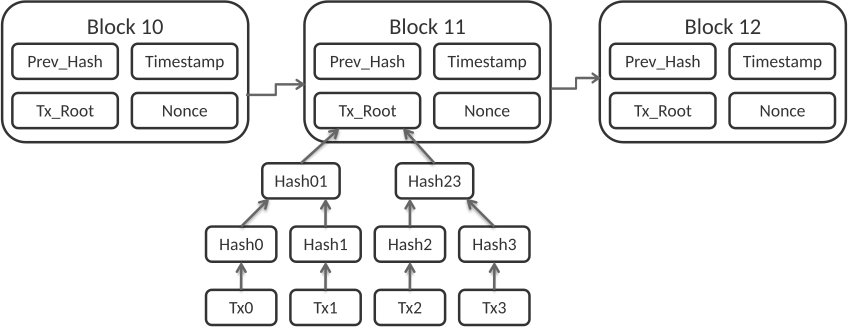
\includegraphics[width=\columnwidth]{figures/Bitcoin_Block_Data.png}
    \caption{Blockchain structure, attribution: Wikimedia Commons~\cite{wikimedia:blockchain}.}
    \label{blockchain-figure}
\end{figure}

\section{What Are Bear and Bull Markets?}
While you may know that the bear and bull markets stand for falling and rising markets, there is more to these terms that must be explained. The origin of the terms themselves is believed to be tied to the way the two animals attack their opponents. A~bull thrusts its horns up, while a bear swipes its pawns downwards~\cite{investopedia-bull-market}.
Herd behavior is important to consider when talking about the terms.

\subsection*{Bear Market}
As growth prospects wane and expectations are unmet, prices decline~\cite{investopedia-bear-market}. Bear markets are viewed as pessimistic, with investors scared to open new positions. But to talk about bear or bull market, we usually ascribe longer time periods than the usual and always present volatility of the crypto market. For example, when China declared all of the cryptocurrency transactions illegal~\cite{china-ban}, a fall of crypto markets quickly ensued.

A~bearish investor or bear is then a type of investor that believes that a specific coin is likely to decline in the future~\cite{investopedia-bull}.

\subsection*{Bull Market}
Bull markets are characterized by optimism, investor confidence and expectations in strong results that will continue for a long period of time~\cite{investopedia-bull-market}. FOMO\footnote{Fear of missing out.} is present among investors. Both bull and bear markets are hard to define, bull market is usually specified to occur when prices rise by $20\%$ after a previous $20\%$ drop and before another $20\%$ drop---these values are defined for stock markets only, so the margins should be higher for the volatile cryptocurrency market.

A~bullish investor or bull is a type of investor that believes that a specific coin is likely to rise~\cite{investopedia-bull}.

\section{What Is a Trading Strategy?}
Trading strategy is traditionally defined as a systematic methodology that is used for buying and selling the selected assets in a market. It is based on predefined rules and criteria that are used to execute a trading decision~\cite{investopedia:trading-strategy}.

In this thesis, a trading strategy is considered a method which tells us whether to buy or sell on a given day based on indicators, such as the current cryptocurrency price, or total market capitalization.

\chapter{Trading Strategies for Cryptocurrencies}
\label{chapter-trading-stategies}

There are various trading strategies available regarding cryptocurrencies.
In this chapter, we will go through those that are considered the most well-known and consider
their ups and downs.

\section{HODL}

This is the strategy that is one of the most prominent in the cryptocurrency market, especially by beginners to trading.
It is jokingly derived from a misspelling of the word "hold". The original post by the user GameKyuubi~\cite{hodl-post} containing the misspelling was originally posted on 18th December 2013, from which it quickly spread on.

HODL or "hold on for dear life" has become a slogan among crypto enthusiasts, representing a long-term approach to cryptocurrency trading. It implies that the novice traders are not successful in timing the market, so they should simply hold the coin until the prices significantly rises.

Cryptocurrency maximalists keep HODLing, because they believe that cryptocurrencies will eventually replace the government-issued fiat currencies as the basis of all economic structures~\cite{investopedia-hodl}.

\section{Rebalance}
\label{section-rebalance}
Rebalancing is the process of realigning the weightings of a portfolio of assets---in our case, cryptocurrencies. It involves periodically buying or selling the assets in the portfolio so that the original level of asset allocation is maintained~\cite{investopedia-rebalancing}.

For example, if we set portfolio allocation 50/50 to BTC and ETH coins. And the BTC coin rised by 20 \% so that the new ratio would be 70/30, we would sell the 20 \% of the BTC and for the value we got we would buy additional ETH coins, so that the ratio is again 50/50.

Rebalancing gives investors the opportunity to sell high and buy low. It takes gains from high-performing investments and reinvests them in areas that have not yet grown that much.

One study~\cite{portfolio-rebalancing}, conducted by the Shrimpy Team, has found that rebalancing beats HODL by a median of $64\%$. The analysis was performed with 1-year period real trading data.

There are many types of rebalancing strategies. We will look at some of them now.

\subsection*{Periodic Rebalancing}
This is the simplest rebalancing to use. The rebalance happens after a fixed amount of time. For cryptocurrencies, it makes sense to set shorter time due to rapid price fluctuations, something like 1 day. An example of periodic rebalancing can be seen in Figure~\ref{periodic-rebalance-figure}.

\begin{figure}[!t]
    \centering
    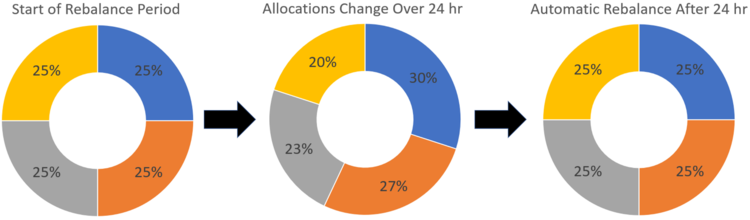
\includegraphics[width=\columnwidth]{figures/periodic-rebalance.png}
    \caption{Periodic rebalance visualization, attribution: Shrimpy~\cite{portfolio-rebalancing}.}
    \label{periodic-rebalance-figure}
\end{figure}

\subsection*{Threshold Rebalancing}
A~more interesting approach is threshold rebalancing, where we set some threshold deviation. When an allocation deviates by that set threshold from the original allocation, a rebalance happens, setting all the allocations to their original values~\cite{portfolio-rebalancing}.

Let's say we once again have 50/50 BTC/ETH allocations. Let's set the threshold deviation to $20\%$. If the price of BTC or ETH reaches over 60\% or under 40\%, a rebalance takes place. 20\% out of 50\% is 10\%, that is why the rebalance happens at those points. When both coins grow or decline in the same rate, no rebalance happens.

An example of threshold rebalancing can be seen in Figure~\ref{threshold-rebalance-figure}.

\begin{figure}[!t]
    \centering
    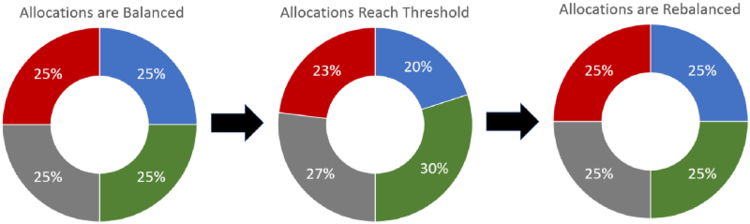
\includegraphics[width=\columnwidth]{figures/threshold-rebalance.png}
    \caption{Threshold rebalance visualization, attribution: Shrimpy~\cite{portfolio-rebalancing}.}
    \label{threshold-rebalance-figure}
\end{figure}

\subsection*{Assumptions}
\label{rebalance-assumptions}
One study around rebalancing has been already mentioned, let's look into some of them in more detail now. The studies~\cite{portfolio-diversity} and~\cite{diversify-perform-better} conducted by the Shrimpy organization have found some interesting results. Both of the studies took into account only periodic rebalancing. They have found that the shorter the time period for rebalance, the better the results, maximizing them at a 1-hour period. The other interesting discovery was that if the portfolio had more assets in it---was more diversified---the better the results are. The diversification really took advantage of the sell high, buy low formula.

Another study~\cite{rebalancing-strategy} confirmed that a portfolio with a larger number of assets performs better. Some other interesting facts have been observed during the simulations that improve the performance of the portfolio:
\begin{itemize}
    \item Equal weightings of the allocated assets.
    \item Assets that are uncorrelated or negatively correlated with each other. That means if one rises, the other should go down.
    \item Assets that have similar rates of return, though volatility also improves the performance.
\end{itemize}

\section{Dollar Cost Averaging}
\label{section-dca}
Dollar Cost Averaging (DCA) is a strategy often recommended to the beginner investors. The investor makes periodic purchases of the asset in an effort to reduce the volatility of the market. This removes much of the detailed work needed to time the market in order to make purchases at the best price.

Through studies~\cite{DCA-study} it seems that the advantage of DCA lies more in the reduced psychological effort in order to time the market than in the actual results. Single buy-and-hold strategy seems to outperform DCA in more cases.

Sometimes DCA is used as a mean to invest into trusted assets on weekly/monthly basis---when employees get money. It is also used in some employment plans\footnote{For example, the American 401(k) plan} across the world.

\section{Day Trading}
Day trading are the investors that buy and sell the same asset over the span of one day. They might even buy and sell the assets multiple times. They mostly use technical analysis of the market to achieve this goal. It is not recommended for beginner investors to choose this type of trading, as it is much more risky than strategies described before.

\section{Range Trading}
\label{section-range-trading}
Asset move in certain ranges, as you can see in Figure~\ref{trading-range-figure}. Range trading assumes that and tries to take guesses where are the limits using candlestick charts and support and resistance levels. Investors want to buy when prices reach the support level and sell when they reach the resistance level~\cite{5types-of-daytrading}. The support and resistance levels can be seen in Figure~\ref{sup-and-res-levels}.

\begin{figure}[!t]
    \centering
    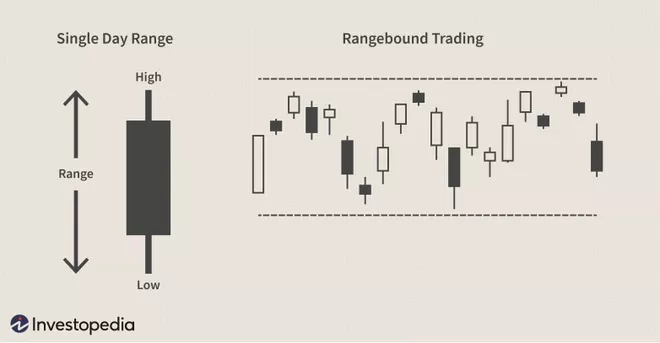
\includegraphics[width=\columnwidth]{figures/trading-range.png}
    \caption{Trading range visualization, attribution: Investopedia~\cite{investopedia:trading-range}.}
    \label{trading-range-figure}
\end{figure}

\begin{figure}[!t]
    \centering
    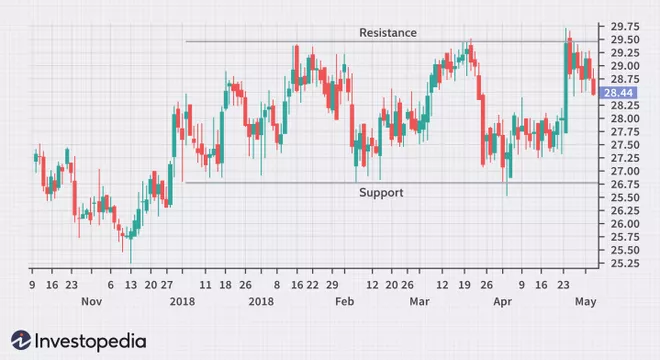
\includegraphics[width=\columnwidth]{figures/dotdash-final-trading-range.png}
    \caption{Support and resistance levels, attribution: Investopedia~\cite{investopedia:trading-range}.}
    \label{sup-and-res-levels}
\end{figure}

\section{Scalping}
\label{section-scalping}
In scalping you try to profit from very small price movements over short periods, you might exit a trade seconds after entering it. It is best to use automated bots to increase the buying frequency. Scalpers take advantage of increased trading volume to profit. They want to exit before any news or short-term fluctuation changes the market's view of the coin~\cite{best-crypto-daytrading}.

A~large bankroll is required for effective use of this strategy. Since the return of investment is really low, the profit made must be significant enough. It also needs to cover trading fees.

In Figure~\ref{scalping-figure} it can be seen how scalping can take quick and short advantages of the market.

\begin{figure}[!t]
    \centering
    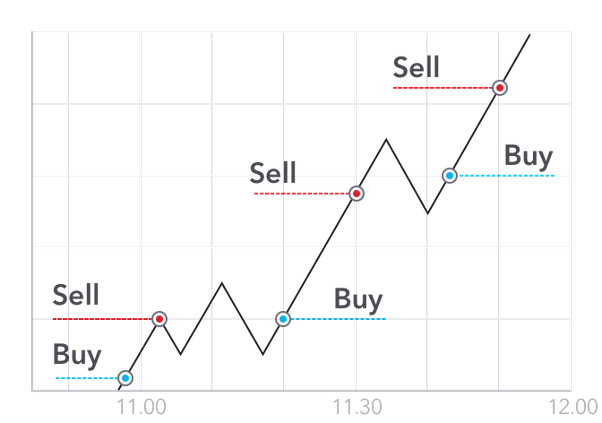
\includegraphics[width=\columnwidth]{figures/scalping.png}
    \caption{Scalping visualization, attribution: Quora~\cite{best-crypto-daytrading}.}
    \label{scalping-figure}
\end{figure}

\section{Automated Trading Systems or Bots}
\label{bots}
Automated trading systems---also referred as algorithmic trading---allow investors to set specific rules for enter and exit of a trade that can be automatically executed via a computer program. Some platforms claim that 70\% to 80\% of trading done comes from the automated systems~\cite{investopedia-bot-trading}.

One of the advantages is that the automated trading systems take emotions out of the trading---they only work on specific criteria. The automated trading systems need to use software or APIs available from the broker. The product of this thesis is expected to be used by these automated trading systems.

Automated trading systems are one of the few options to use when considering strategies like scalping due to the ease of getting in and out of a trade in seconds without room for failure. The software also allows backtesting the chosen strategy on historical data, from which it can be seen how well it does perform.

\section{Arbitrage}
Arbitrage involves buying cryptocurrency in one market and selling it for higher price in another one. Since the cryptocurrency market is usually unregulated, anyone can make an exchange. This can lead to major differences in the spread of the asset.

There are two types of arbitrage when it comes to cryptocurrencies. The first one focuses on finding prices mismatches across different trading pairs on a single exchange. The other is the one that was already described---locating significant price differences on multiple exchanges. Both types take advantage of an automated trading system that monitors the exchanges and looks for price differences. In Figure~\ref{arbitrage-figure} you can see how the first type can be profitable.

Regarding the second type of exchange. In January, a legendary \emph{kimchi premium}\footnote{\url{https://www.investopedia.com/terms/k/kimchi-premium.asp}} happened. Bitcoin traded almost 40\% higher on the Korean exchanges than the US exchanges. This lead to arbitrage investors taking advantage of this fact, buying Bitcoin on US exchanges and selling it on the Korean ones for profit~\cite{hodlbot:day-trading-cryptocurrency}.

\begin{figure}[!t]
    \centering
    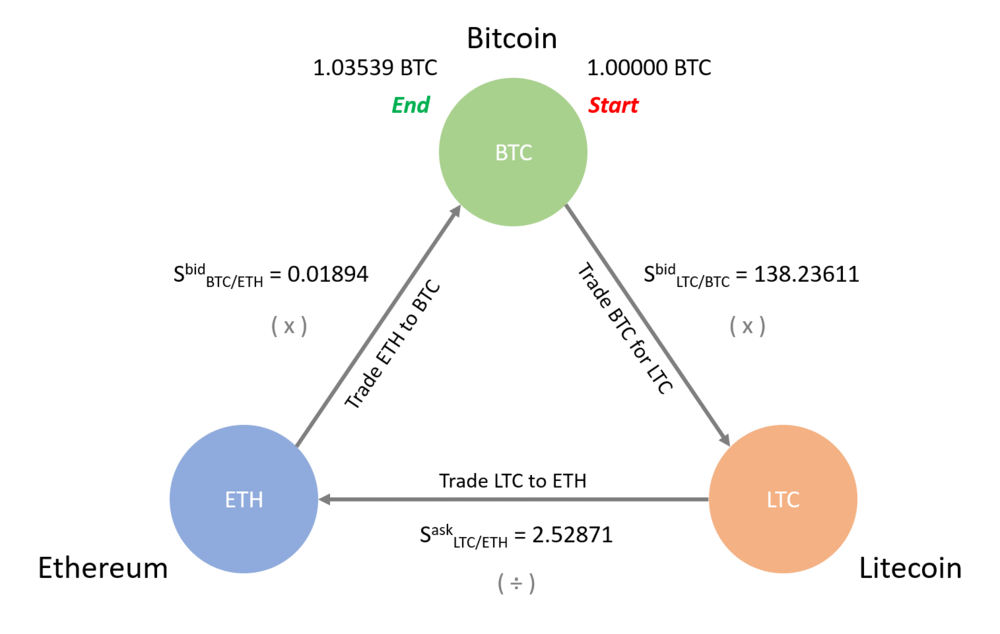
\includegraphics[width=\columnwidth]{figures/arbitrage.png}
    \caption{Arbitrage execution via multiple trading pairs, attribution: HodlBot~\cite{hodlbot:day-trading-cryptocurrency}.}
    \label{arbitrage-figure}
\end{figure}

\section{Stablecoin Trading}

When talking about different trading strategies, the focus is usual on the method of the strategy, not the asset themselves. But when it comes to a specific thing like stablecoins, there is an opportunity to handle them in such a way to generate profits for investors.
The term stablecoin has already been explained in~\ref{stablecoins-ref}. It is a coin which has its value pegged to some external reference.

For example, it was found in~\cite{make-money-stablecoins} that a de-pegging of stablecoins happens periodically often as a result of temporary shock to the crypto system. During those events profit can be made when trading pegged and de-pegged stablecoins between each other. The author chose the stablecoins DAI\footnote{\url{https://coinmarketcap.com/currencies/multi-collateral-dai/markets/}} and USDC\footnote{\url{https://coinmarketcap.com/currencies/usd-coin/}} for their experiments. It was shown that between August 2019 and March 2020 the spread between DAI and USDC has been fluctuating between 2 to 3\%. Advantage could be taken of this fact---selling DAI for USDC when the price is high and buy it back for USDC when the price returns to the peg.

One thing to remember is to only trade when the spread is sufficient so that the trading fees won't make the profit diminish.

\chapter{Existing Simulation Tools for Testing Trading Strategies}
\label{chapter-simulation-tools}

In this chapter different simulation tools, their application, usefulness and differences, are discussed. When discussing simulation tools, their different types must be distinguished. When novice investors first set foot in the cryptocurrency market, they might be startled by the complexity of the market. They want to learn, but maybe they do not want to lose all their money in the process. That is the perfect opportunity for a manual simulated tool. Investors can invest fake virtual money while all the market's trading data is accurate and up to date.

\section*{Types of cryptocurrency simulators}

\begin{enumerate}
    \item Cryptocurrency market games
    \item Virtual trading simulators
    \item Backtesting simulation tools
\end{enumerate}

\emph{Cryptocurrency market games} are games that have less emphasis on the trading skills and more on the entertainment of trading. They are mostly a fun way to compete with your friends or strangers. The player that creates the strongest portfolio is considered the best. The winner is then the player with the best investments at the end of the specific game.~\cite{top-stocks-crypto-trading-simulators}.

\emph{Virtual trading simulators} are simulators where users can closely track the real market and actively trade cryptocurrencies for virtual profit~\cite{top-stocks-crypto-trading-simulators}. The main goal is to use the simulated experience for building and improving the real life trading skills of the user. You can test-drive and backtest your strategy with these.

\emph{Backtesting simulation tools} are similar to the virtual trading simulators in a way, that it aims to make its users better at trading. While the conventional trading simulators only work in real time, there are simulation tools where its users can input a chosen strategy and see it run across multiple years of historical data and see how it performed in seconds. This is the type of simulation tool that will be used in this thesis. It basically uses backtesting for the cryptocurrency strategy's validation.

\section{What Is Backtesting?}
The section was inspired by the Bybit article about backtesting cryptocurrency strategies~\cite{backtesting-crypto-trading-strategies}.

Backtesting means applying a trading strategy or some analytical method on historical data and analyzing the performance of the current strategy or method. If the strategy shows promise, the trader may use it in a live environment on an exchange. Backtesting does not guarantee future results, but can be a good indicator and filter the effective strategies from the ineffective ones. Backtesting can also detect recurring patterns and exploit those patterns for profits.

\subsection*{Discretionary Backtesting}
Discretionary backtesting is a manual form of backtesting. The trader manually places buy and sell orders with each signal they receive. The trader may decide to conduct the testing using software such as TradingView\footnote{\url{https://www.tradingview.com/}}.

The trader will set a strategy in place, then he will press the replay button (shown in Figure~\ref{tradingview-figure}) and select a period of history to test on. The trader will then make discretionary decisions to buy or sell based on the signals.

Manual testing is a great way to control trader's emotions since they may feel the same emotions as in live environment. The disadvantage is that it is quite time-consuming. A~trader may run a test for hours only to find out it was not a good strategy (though this result is also valuable). Secondly, the amount of data the trader can test the strategy on is limited.

\begin{figure}[!t]
    \centering
    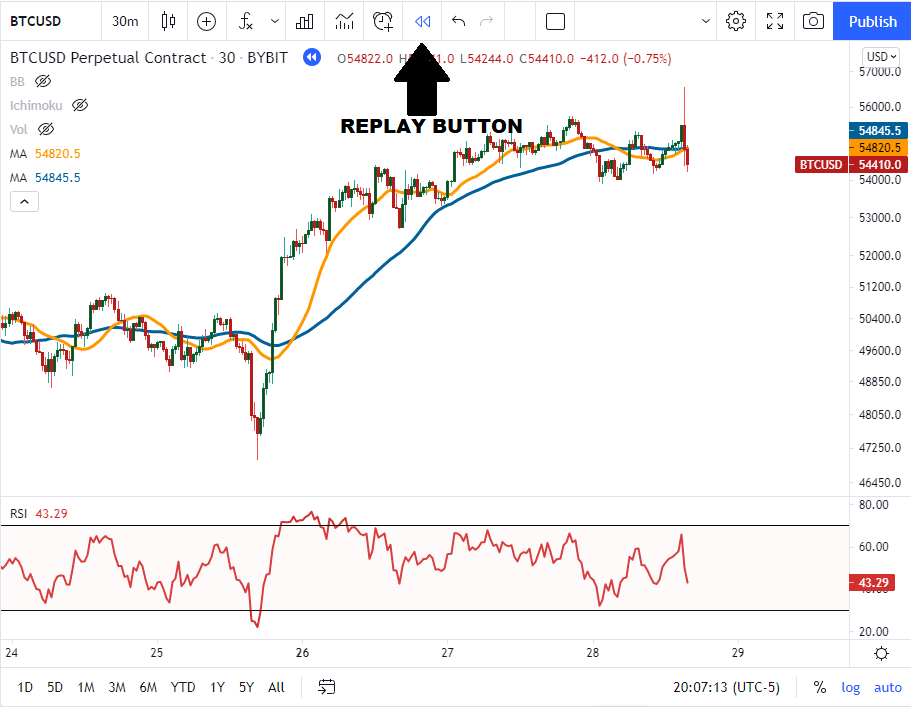
\includegraphics[width=\columnwidth]{figures/tradingview-replay.png}
    \caption{TradingView replay functionality, attribution: TradingView~\cite{backtesting-crypto-trading-strategies}.}
    \label{tradingview-figure}
\end{figure}

\subsection*{Systems Backtesting}
Systems backtesting offers the trader the true power of technology. Systems traders will have a strategy coded, and the program will test the strategy against the historical data while generated statistics of the achieved results in manner of seconds. This will show the trader useful statistics about the strategy and help him decide if it is robust and well-performing enough to use in a live environment.

The challenge of systems backtesting is to have sufficient technical knowledge on how to create such algorithmic strategies. And also the analytical knowledge to determine if the strategy performed well or not.

\subsection*{Automated Backtesting}
Automated or \emph{algorithmic} trading refers to traders who use a computer program to execute a trade, as explained in~\ref{bots}. Backtesting of strategies can also be automated this way and is usually just another name for systems backtesting. We automate the results to arrive at helpful statistic to help us determine effective strategies. It is conducted using a programming language.

\subsection*{Simulated Backtesting}
Simulated backtesting simply means running a test over a historical data that simulates the real market environment. In this example, the system is the market environment and the model is the simulated backtesting.


\section{Data Requirements for Backtesting}
Systems traders will want to simulate the real-world data as closely as possible. Trading costs such as commissions, exchange spreads and slippages can chew away the expected returns. This costs can throw off the backtest results if ignored.

Both \emph{candlestick} and \emph{order book data} are used in backtests, though order book data is usually more reliable.

\subsection*{OHLCV Candlestick Data}
\label{ohlcv-candlestick-data}
OHLCV stands for Open-High-Low-Close-Volume, you can see how they can be represented in Figure~\ref{OHLCV-figure}. The candlestick data itself is visualized in Figure~\ref{candlestick-figure}. It is essentially a spreadsheet of price data of the chart time frame. If you pull the candlestick data for the daily chart of Bitcoin, you will receive each day's open, high, low, and close price data. If you request 1-minute data, the spreadsheet will include each minute's open, high, low, and close price for Bitcoin on that particular day.

OHLCV abbreviations explained~\cite{kaiko-ohlcv}:
\begin{itemize}
    \item Open: Price at which the asset started at the time interval.
    \item High: Highest price reached during the time interval.
    \item Low: Lowest price reached during the time interval.
    \item Close: Price at which the asset ended after the time interval.
    \item Volume: Quantity of asset bought or sold, displayed in base currency.
\end{itemize}

\begin{figure}
    \centering
    \begin{subfigure}[t]{0.45\textwidth}
        \centering
        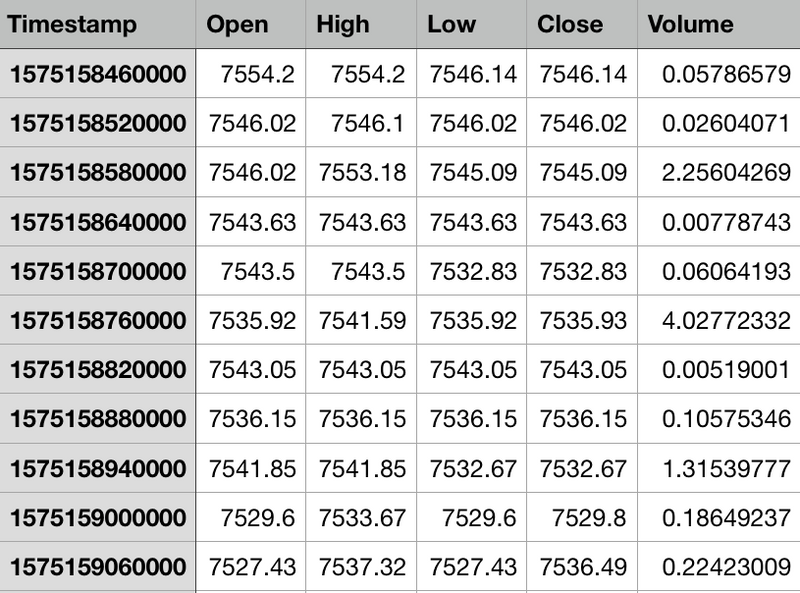
\includegraphics[width=\textwidth]{figures/OHLCV-data.png}
        \caption{How can OHLCV data look like, attribution: Kaiko~\cite{kaiko-ohlcv}.}
        \label{OHLCV-figure}
    \end{subfigure}
    \hfill
    \begin{subfigure}[t]{0.45\textwidth}
        \centering
        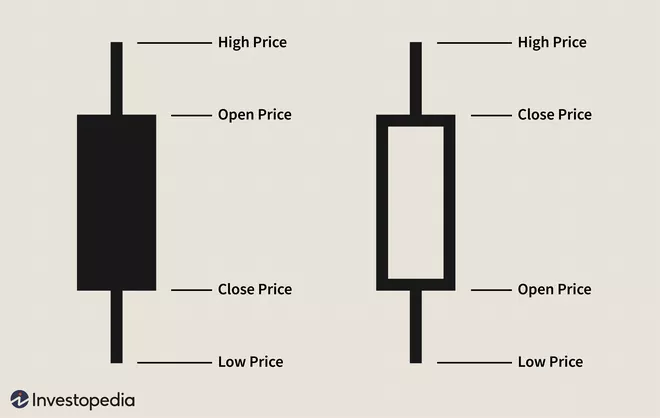
\includegraphics[width=\textwidth]{figures/candlestick-data.png}
        \caption{Candlestick explained, attribution: Investopedia~\cite{investopedia:candlestick-charts}.}
        \label{candlestick-figure}
    \end{subfigure}
    \caption{OHLCV Candlestick Data.}
\end{figure}

There are several imperfections in the OHLCV candlestick data. Firstly, there is no information which prices have been traded for which volume. Additionally, if a trader has a large account, there might not be enough cryptocurrency available to trade without moving the market price---negatively impacting the backtest results. Traders typically use candlestick data because it is easiest to acquire.

\subsection*{Order Book Data}
An order book is one of the best data sources and resolves some challenges of the candlestick data. It includes snapshots of the market, including the market's price, volume and depth. With this type of data, traders have a better representation of what orders are available at any given time.

It allows testers to simulate bid-ask spread, slippage and liquidity when testing a particular strategy. All of these are unavailable to testers using candlestick data. The challenge with order book data is that it is hard to come by. There is a tremendous amount of data with order book snapshots, so the exchanges choose not to hold the data, as it would be too expensive to store. Therefore, usually the developers need to collect and store the data from the exchange themselves or access the snapshots through a third-party service.

\section{Performance Analysis}
\label{performance-analysis}
The section was again inspired by the Bybit article about backtesting cryptocurrency strategies~\cite{backtesting-crypto-trading-strategies}.

Performance of the given trading system or strategy is commonly gauged against parameters such as profit and loss (P\&L), success ratio, and Sharpe ratio.

\subsection*{Profit and Loss -- P\&L}
Once the desired strategy has been created and backtest executed, the thing traders will be interested in is the profit. The backtest should spit out P\&L analysis by trade and day. That way an equity curve can be created, showing what the balance would have been if it were traded live. Equity curve is just a time series chart showing what the value of the account would have been after each passed day.

P\&L analysis also generates the size of the average winning and the size of the average losing trade. Taking the ratio of those two averages, you get a useful average risk-to-reward ratio. For example, if the average winning trade is \$100 and the average losing trade is \$50 you get a $1:2$ risk-to-reward ratio.

\subsection*{Success Ratio}
The success ratio is the win ratio of the strategy. Let's say a strategy makes 100 trades. If 72 of those trades are profitable, it has 72\% success (or win) ratio. By itself, the ratio does not tell much and might be misleading. It is best coupled with the average winner and the average losing trade ratios mentioned in P\&L.

For example, a success ratio of 58\% and 1:2 risk-to-reward ratio indicates a very good strategy.

\subsection*{Sharpe Ratio}
This subsection was sourced from~\cite{investopedia:sharpe-ratio}

The Sharpe ratio, developed by \emph{William F. Sharpe}, is used to understand the return of an investment (ROI) compared to its risk. The ratio is the average return earned in excess of the risk-free rate per unit of volatility or total risk.

$$Sharpe\ ratio = \frac{R_p - R_f}{\sigma _p}$$
where:
\begin{itemize}
    \item $R_p$ = return of portfolio
    \item $R_f$ = risk-free rate
    \item $\sigma_p$ = standard deviation of the portfolio's excess return
\end{itemize}

Generally, the greater the value of the Sharpe ratio, the more attractive the risk-adjusted return. The yield for the US Treasury bond is often used as the risk-free ratio. One of the limitation of the Sharpe ratio is that it assumes that the returns are normally distributed, which is simply not true. Financial markets are not normally distributed, because of large number of surprising drops and spikes in the price. Additionally, it would mean that price movements in either direction is equally risky. The financial reality tells us that that is not the case.

\section{Popular Simulation Tools}
Some popular and easily available simulation tools are Holderlab,\footnote{\url{https://holderlab.io/}} Zenbot,\footnote{\url{https://github.com/DeviaVir/zenbot}} Gekko,\footnote{\url{https://gekko.wizb.it/}} Altrady,\footnote{\url{https://www.altrady.com/}} and Binance's Python backtesting\footnote{\url{https://www.binance.com/}}.

\section{What Type of Cryptocurrency Simulation Tool Should We Use?}
When looking at the explored simulation tools, it is clear that an automated backtesting program will be used to test the proposed adaptive trading strategy. I~will use the OHLCV candlestick data provided by the supervisor and look for order book data if needed. When evaluating the strategy I~will not only look at P\&L ratio, but also the average winner and losing trades, risk-to-reward ratio and more complex tools like Sharpe ratio.

\subsection*{Programming Language}
When looking at possible languages to use, I~consider available libraries and frameworks. I~decided to use Python for its many available trading and backtesting frameworks and because of my personal experience with it for data collection.

\subsection*{Backtesting Frameworks}
Let's look at the available backtesting frameworks for Python. Using frameworks might make things easier for us. Between the candidates for backtesting frameworks I~put PyAlgoTrade, bt, backtrader, zipline and Blueshift. Apart from that, \emph{numpy},\footnote{\url{https://numpy.org/}} \emph{pandas}\footnote{\url{https://pandas.pydata.org/}} and \emph{matplotlib}\footnote{\url{https://matplotlib.org/}} libraries will be probably of great use for general data transformation and visualization. The following section's lines have been inspired by~\cite{python-backtesting-frameworks} source.

When reviewing backtesting frameworks it's always good to ask what asset classes you are trading, what data frequency and detail is required and what order type should be supported by the chosen framework. Some frameworks go beyond backtesting and include live trading capabilities that make it easier for potential deployment.

The framework should have a way to consume trading data in a convenient way. It should calculate a broad range of risk and performance metrics as explained in~\ref{performance-analysis}, including the max drawdown and Sharpe and Sortino ratios.

Computer resources may be a problem sometimes. Traders can opt for frameworks with distributed or parallel processing in those scenarios. When it comes to strategy optimization, the program may attempt to find the optimal parameters for each technical indicator, testing various combinations. In portfolio context, the program may try to find the best weighting of every asset in the portfolio for the ideal rebalance.

We will now look at a few backtesting frameworks for Python and lightly compare them. The common capabilities of the frameworks is that they are event driven, with flexible licenses, having a decent number of pre-defined technical indicators and standard performance metric calculation, visualization and reporting capabilities.

\emph{PyAlgoTrade}\footnote{\url{https://github.com/gbeced/pyalgotrade}} is a fully documented framework with paper and live trading capabilities. Its data support includes Yahoo! Finance, Google Finance, NinjaTrader and any type of CSV-based time series.

\emph{bt}\footnote{\url{https://pmorissette.github.io/bt/}} is used to test quantitative trading strategies. It allows traders to easily create strategies that mix and match different algorithms. It aims to save developers time re-inventing the wheel and instead focus on the strategy development.

\emph{backtrader}\footnote{\url{https://www.backtrader.com/}} is a feature-rich backtesting framework. It allows you to focus on writing reusable trading strategies, indicators, and analyzers rather than on building the infrastructure itself.

\emph{Blueshift}\footnote{\url{https://blueshift.quantinsti.com/docs/}} is a platform to research and test systematic investment strategies. It is asset-class and instruments agnostics. It is not meant for HFT---high frequency trading.

\emph{Zipline}\footnote{\url{https://github.com/quantopian/zipline}} is an event-driven system for backtesting. It is accessible through the browser-based IPython Notebook interface, which makes it available to developers who do not prefer the command line.


\chapter{Trading Data Analysis}
\label{chapter-data-analysis}

In this chapter, the historical data of cryptocurrency market is analyzed. We try to find trends and patterns that we can then use to our advantage when coming up with an adaptive trading strategy.

\section{Types of Analysis}
This section was inspired by the Binance Academy article about Bitcoin's price history~\cite{binance:bitcoin-price-history}.

Before we analyze the cryptocurrencies themselves, let's take a look at ways how to analyze them. There are generally three possible methods: technical, fundamental and sentiment analysis. Each type has its strengths and weaknesses. Combining them together creates a clearer picture.

\subsection*{Technical Analysis -- TA}
The main focus here is on the historical price and volume data. We can create a 50-day moving average (SMA) by taking the last 50 days' prices and averaging them. If a cryptocurrency has been trading under its 50-day SMA for a few weeks and suddenly breaks through, it may be seen as a sign of possible recovery. The technical analysis is the analysis mostly used in the thesis.

\subsection*{Fundamental Analysis -- FA}
Fundamental analysis takes its merits from the fundamental, intrinsic value of a project or cryptocurrency. It concentrates on internal and external factors to try to establish the asset's actual value. For example, you could take a look at daily cryptocurrency's transaction to measure the network's popularity. If the number of transactions rises over time, it may suggest the value of the project and that its price may rice.

\subsection*{Sentiment Analysis -- SA}
Sentiment analysis is the use of market sentiment to predict the price movements. Market sentiment represents the feelings and mood of investors towards an asset. These are typically categorized into bullish and bearish sentiments. A~significant increase in google searches about purchasing some cryptocurrency may suggest a market sentiment.

\section{Bitcoin Price Analysis}
This Section was inspired by the Binance Academy article about Bitcoin's price history~\cite{binance:bitcoin-price-history} and Investopedia's article on Bitcoin's price history~\cite{investopedia:bitcoin-price-history}.

First thing to analyze is Bitcoin in particular. No other cryptocurrency has such an impact on the cryptocurrency market, something which it continues to do to this day. Since bitcoin is the original cryptocurrency that started this all, it is only appropriate to begin our analysis with it. We can see the linear and logarithmic graphs in Figures~\ref{btc-linear-figure} and~\ref{btc-log-figure} respectively.

While the linear graph shows us the actual price changes, the logarithmic graph is also useful to us. It shows us relative price increases of the Bitcoin. It represents a percentage increase in price, the change from \$10 to \$20 is the same as \$1000 to \$2000 since the investor will in both cases gain a profit of 100\%. Because of this, logarithmic scale is usually often used for technical analysis.

\begin{figure}[!t]
    \centering
    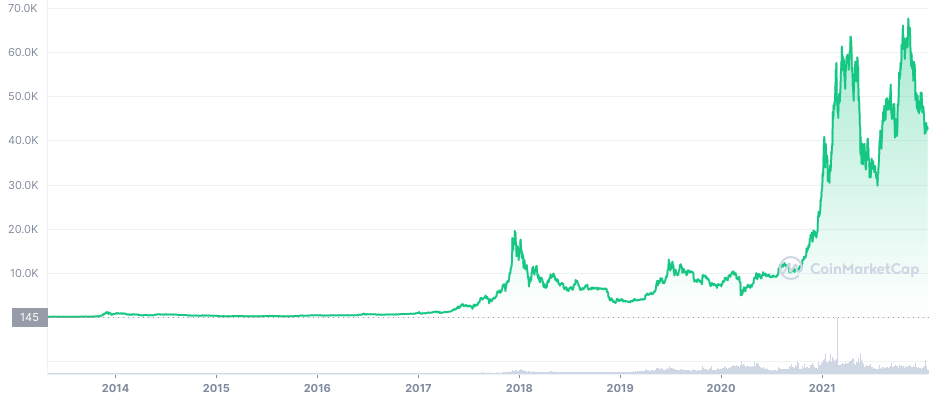
\includegraphics[width=\columnwidth]{figures/BTC_ALL_linear.png}
    \caption{Bitcoin linear price graph, attribution: CoinMarketCap~\cite{coinmarketcap}.}
    \label{btc-linear-figure}
\end{figure}

\begin{figure}[!t]
    \centering
    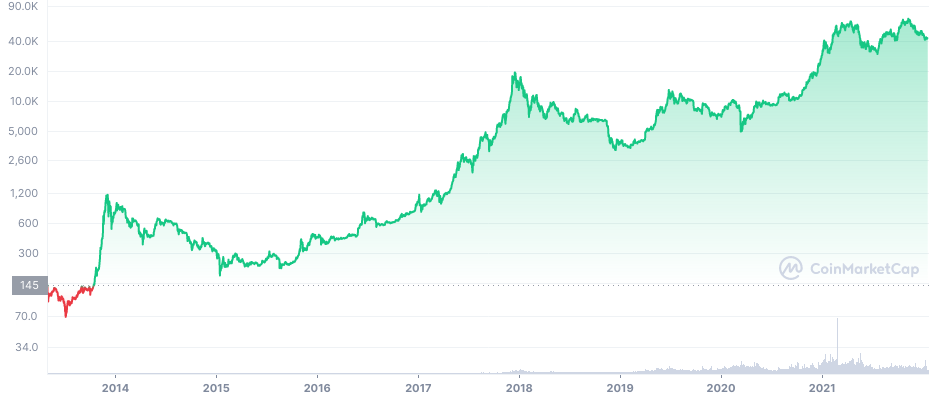
\includegraphics[width=\columnwidth]{figures/BTC_ALL_log.png}
    \caption{Bitcoin logarithmic price graph, attribution: CoinMarketCap~\cite{coinmarketcap}.}
    \label{btc-log-figure}
\end{figure}

Bitcoin's history is nicely presented in Figure~\ref{figure-investopedia-btc-history}. When Bitcoin was introduced in year 2009, it had a price of zero. It took until July 17, 2010 for the price to jump to mere \$0.09. From April 2011 to June 2011 the Bitcoin gained 2,960\%, rising from \$1.0 and peaking at \$29.60. A~recession followed, and Bitcoin bottomed out at \$2.05 by November. 2012 proved to be a generally uneventful year for Bitcoin. 2013 again witnessed strong gains in price. It reached \$230 in April. In December, the Bitcoin spiked to \$1237 and fell to \$687 three days later. 2014 did not register any major spikes. During the years of 2015 and 2016, the prices slowly climbed, reaching over \$900 by the end of 2016.

In 2017, Bitcoin's price hovered around \$1,000 until it broke \$2,000 in May. It skyrocketed on December 15 to \$19,345. That is where the Bitcoin gained its first huge media coverage. Mainstream investors, governments, economics took notice. Other cryptocurrencies began quick developing to compete with the Bitcoin. Bitcoin's price moved sideways during the next two years, with small bursts of price.

When the economy shutdown in 2020 due to the COVID-19 pandemic---Bitcoin woke up once again. The cryptocurrency started the year around \$7,000. The shutdown combined with subsequent government policy made investors fearful about the global economy and accelerated Bitcoin's rise. On 23rd November, Bitcoin was trading at \$19,157. Bitcoin's price rose to just under \$29,000 in December 2020, increasing 416\% from the start of the year.

Bitcoin took less than a month of 2021 to beat the record of 2020, surpassing \$40,000 by January 7. By mid-April, Bitcoin reached a new all-time high of over \$60,000 as Coinbase,\footnote{\url{https://www.coinbase.com/}} a cryptocurrency exchange, went public in the stock market. Bitcoin was once again in the front of the media coverage, which propelled its price more upwards, to the peak of \$63,000 on April 12, 2021.

By the Summer, prices went down by 50\%, hitting just under \$30,000 in July. Another bull run started in September, with prices scraping \$52,600, but it was taken down to \$40,700 two weeks later. On November 10, Bitcoin reached its all-time high once again, \$68,990. In December 2021, prices fell down again as uncertainty about inflation alongside the new COVID-19 variant, Omicron, began to scare the investors.

From the observed events, we can see that media coverage drives the price upwards. And that Bitcoin is susceptible to economic circumstances, as seen during the COVID-19 pandemic. One other interesting fact is that on June 9, 2021, El Salvador made Bitcoin legal tender---meaning it can be used for any transaction where business accept it. It is the first country to do this to this day.

\begin{figure}[!t]
    \centering
    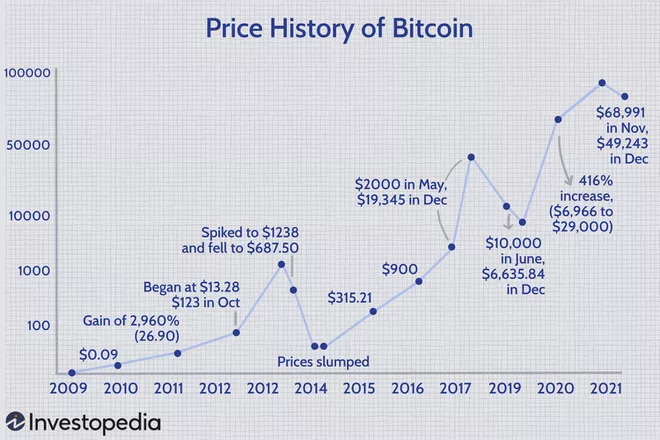
\includegraphics[width=\columnwidth]{figures/investopedia-bitcoin-price-history.png}
    \caption{Bitcoin's price history in detail, attribution: Investopedia~\cite{investopedia:bitcoin-price-history}.}
    \label{figure-investopedia-btc-history}
\end{figure}

\subsection*{Elon Musk Tweets}
This Section has been inspired by the Vox article~\cite{vox:elon} and the CoinDesk article~\cite{coindesk:elon}

One of the most influential figure when it comes to his tweets is Elon Musk, and when it comes to the cryptocurrency market, it applies in double. The price roller coaster of 2021 started when Elon Musk tweeted that Tesla would no longer accept Bitcoin as payment due to environmental concerns. In a result, the price of Bitcoin dropped by 15\%. After suggesting that Tesla is selling Bitcoin, the price continued to plummet down. The next tweet stabilized the market for a bit, Musk ensured that Tesla has not sold any Bitcoin. A~broken heart emoji with the \#Bitcoin hashtag ensured another fall. A~price has however begun to rise once again, when Mush had tweeted that Tesla would once again start accepting Bitcoin.

The whole event can be seen in Figure~\ref{figure-vox-elon}.

\begin{figure}[!t]
    \centering
    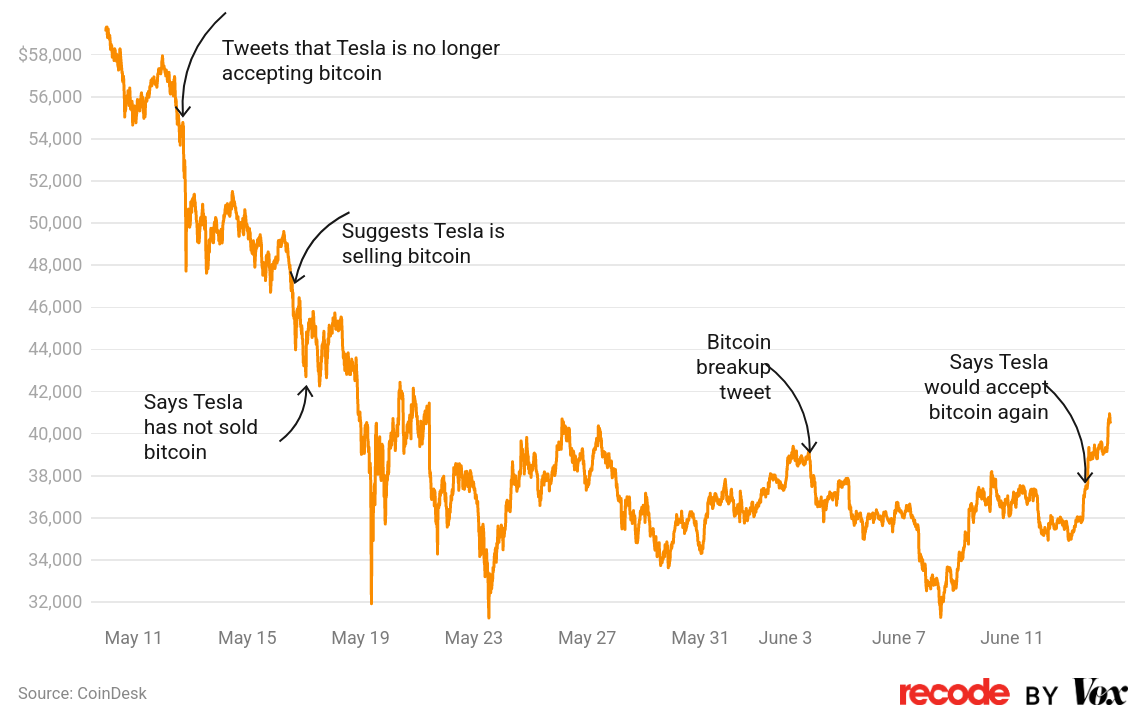
\includegraphics[width=\columnwidth]{figures/vox-elon.png}
    \caption{Bitcoin's price correlation with Elon Musk's tweets, attribution: Vox~\cite{vox:elon}.}
    \label{figure-vox-elon}
\end{figure}

Similar events transpired, but with the Dogecoin\footnote{\url{https://coinmarketcap.com/currencies/dogecoin/}} cryptocurrency in mind. The observed events can be seen in Figure~\ref{figure-coindesk-elon}.

\begin{figure}[!t]
    \centering
    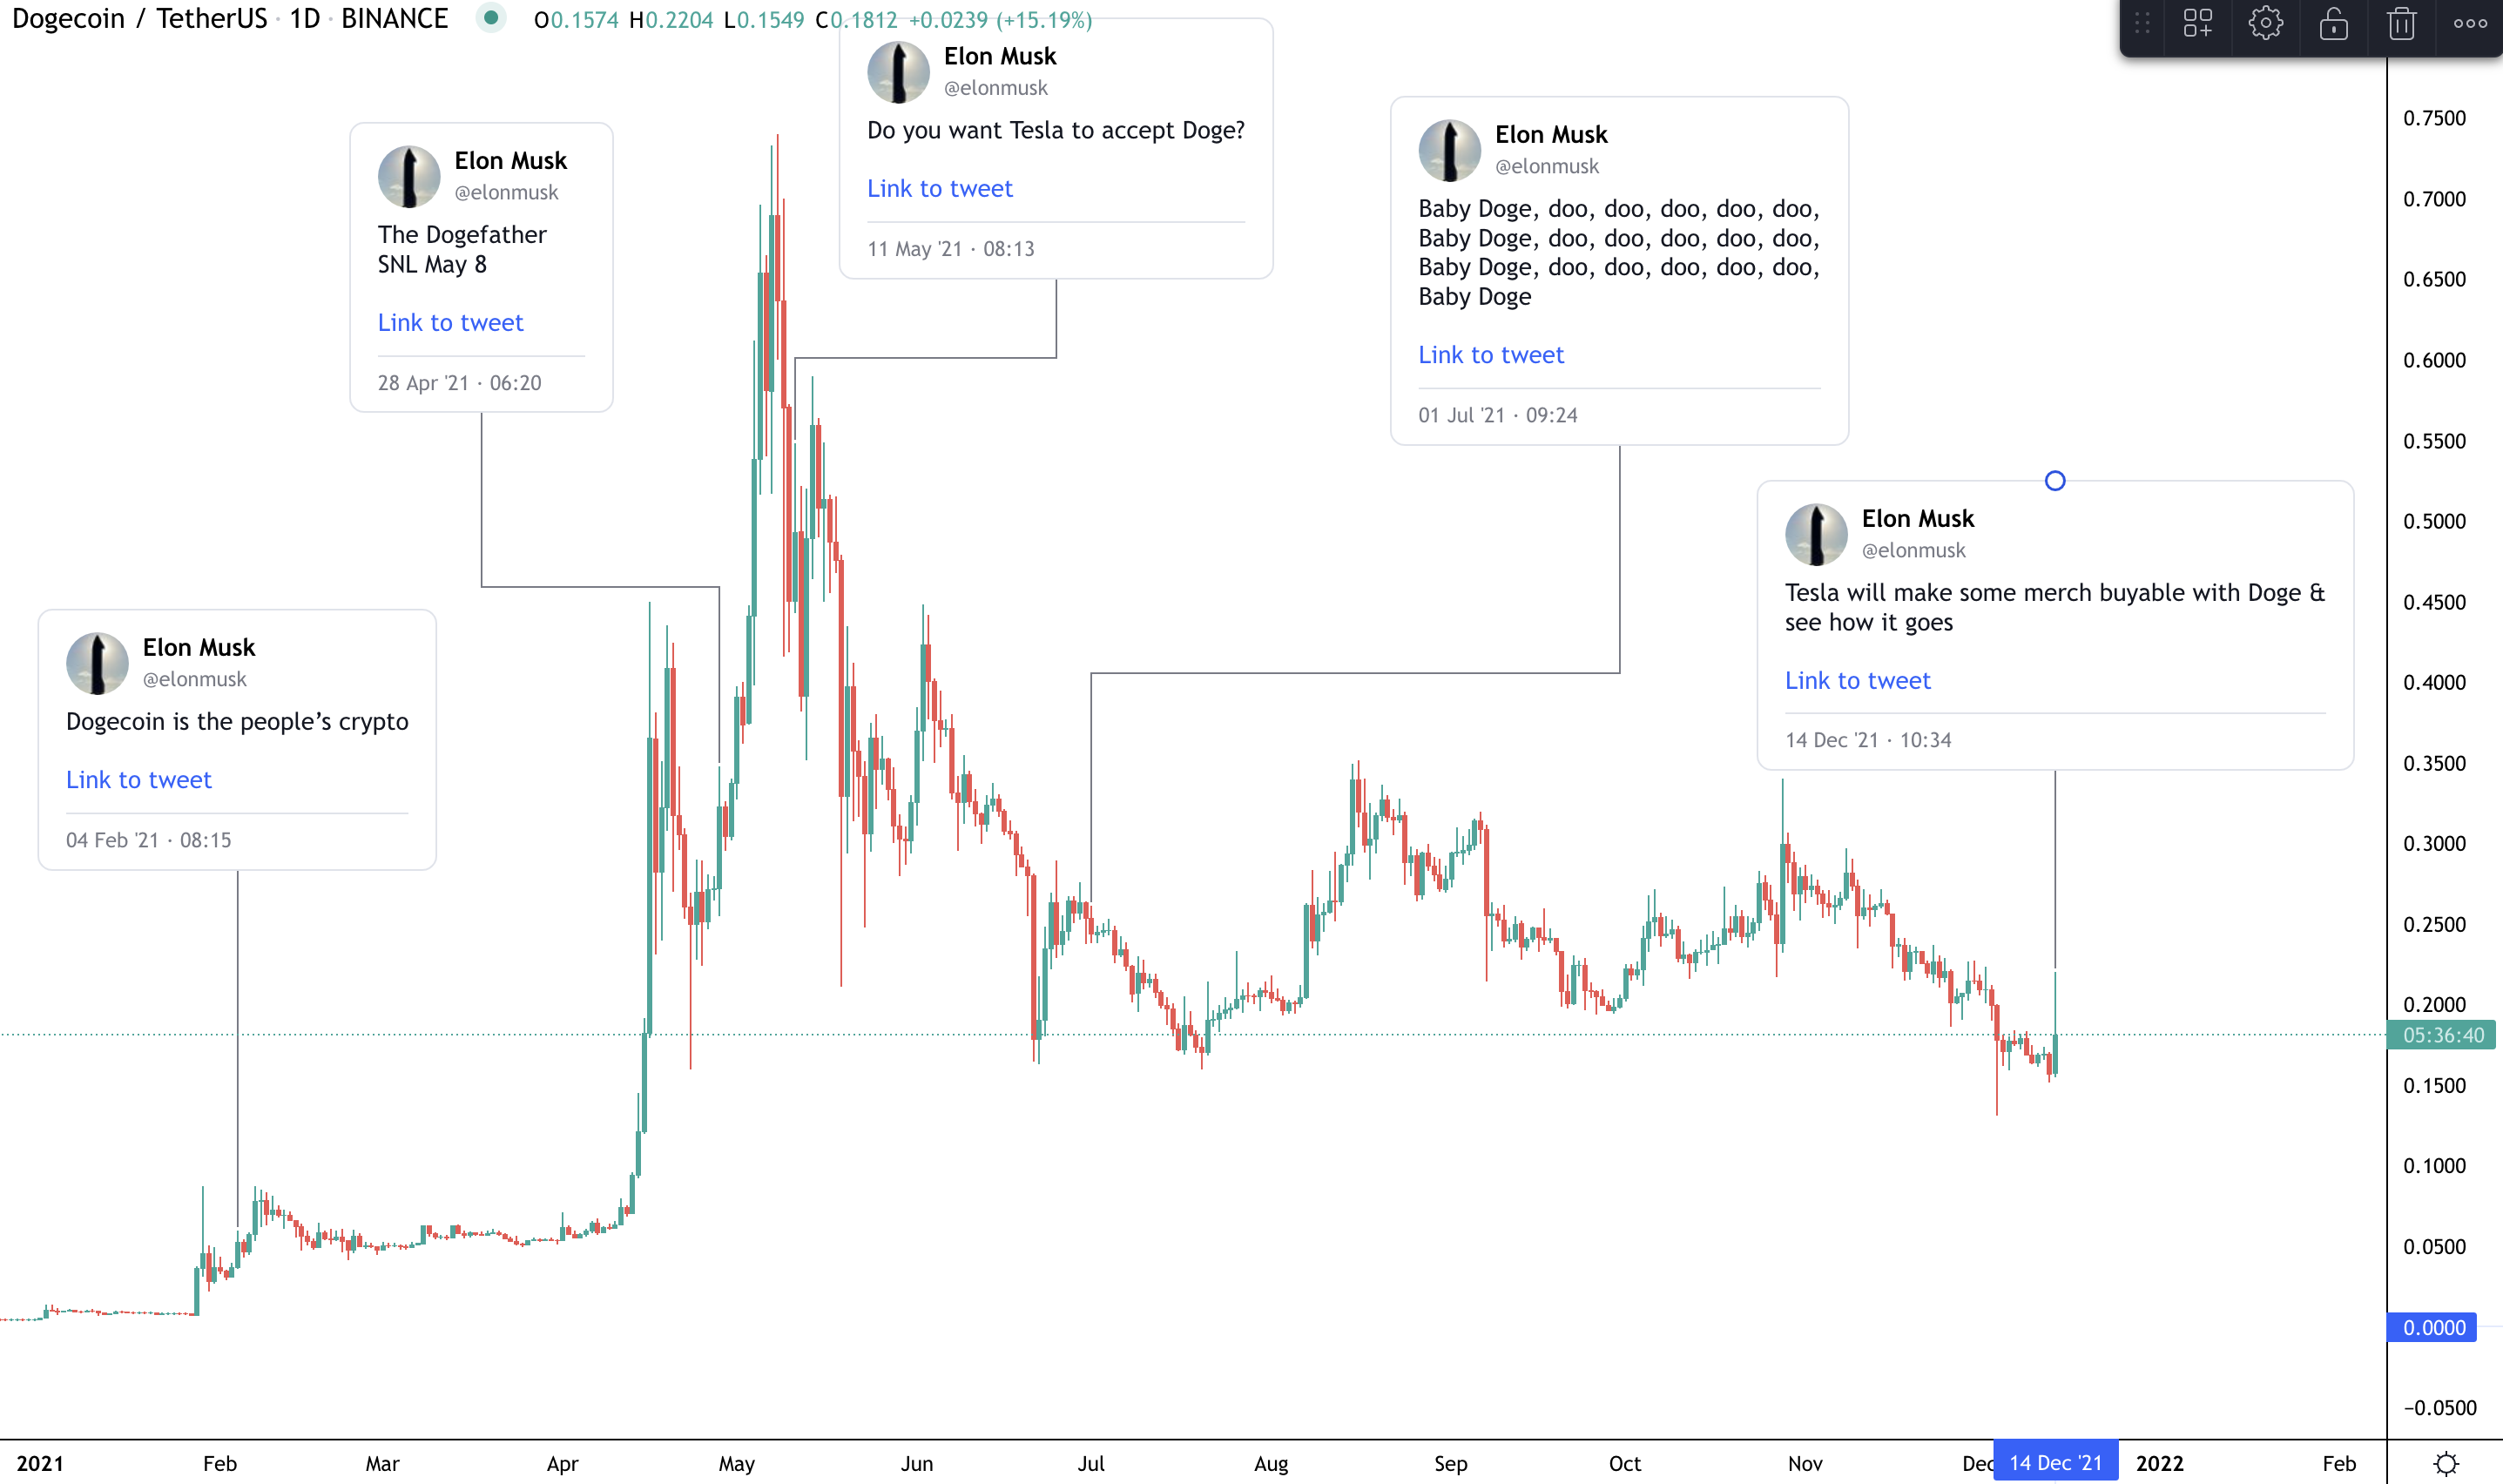
\includegraphics[width=\columnwidth]{figures/coindesk-elon.png}
    \caption{Dogecoin's price correlation with Elon Musk's tweets, attribution: CoinDesk~\cite{coindesk:elon}.}
    \label{figure-coindesk-elon}
\end{figure}

As the reader can see, there is a correlation between Elon Musk's cryptocurrency tweets and the cryptocurrency prices. A~quick reaction to his tweets may lead to significant profits when acted out accordingly, since there is a time before the market catches up with the tweets.

\subsection*{China Ban on Cryptocurrencies}
After the China ban on cryptocurrency trading and mining in May 2021~\cite{china-ban-2}, the Bitcoin price fell down. It followed one week after Elon Musk's tweet about Tesla no longer accepting Bitcoin. These joint events showed that media coverage and world events can easily influence the price of Bitcoin, especially when combined.

\subsection*{What Influences the Price of Cryptocurrencies?}
Since most coins are dependent on the Bitcoin's price movement~\cite{investopedia:altcoins}, by studying what influences Bitcoin, we can understand how other coins act. The prices firstly depend on the perceived value and supply and demand~\cite{investopedia:bitcoin-price-history}. If people believe a cryptocurrency is worth a specific amount, they purchase it, especially if they think it will increase in price. Since there will ever be only 21 million Bitcoins in circulation, the closer the supply gets to the limit, the higher the price should be.

As described above, media coverage, regulation and other world news can easily influence the price of cryptocurrencies. Some interesting implications can be made. By closely (preferably in an automated way) watching the world news and reacting quickly, a considerable profit can be made.

\chapter{Adaptive Strategy Design and Implementation}
\label{chapter-implementation}

Before we get to the strategy proposals, the design and implementation of the backtester program, used to test and analyze the strategies, needs to be discussed. The strategy proposals are immediately supported by implementation and useful Figures in this way. And it is more logically presented in this way, since the implementation is tied to the proposals themselves.

\section{Solution Design}
During my research, I~initially tinkered with several frameworks to test out their capabilities. The basic idea was that if a framework would prove \emph{satisfactory}, I~would use it and tweak it to my needs, so I~do not reinvent the wheel again. A~satisfactory framework in my definition would be easy to work with, easy to learn, and matched to the needs of the proposed adaptive strategies.

Unfortunately, during my tinker with Python frameworks as \emph{PyAlgoTrade}, \emph{backtrader} or \emph{zipline}, the frameworks were either outdated or they did not meet my needs of adaptive strategies.

\subsection*{vectorbt}
One of the more promising frameworks was the \emph{vectorbt} library. I~did a few basic graphs and strategies with it like HODL and MA (moving average) crossover, the examples can be seen in the code. Unfortunately, the library also proved to be insufficient, or more well put, overly complicated, when it came to my needs. Rather than spending days trying to understand a few functions from the library, I~decided it would be faster to create my own backtesting framework that would serve the strategies perfectly while still understanding the inner working of the framework completely. This point was also supported by the thesis supervisor and discussions I~found on the internet~\cite{reddit:custom-backtester}.

\subsection*{General Design}
The general idea is to build a backtesting command line interface (CLI) application. It takes input arguments from the CLI or a configuration file and passes it to the argument parser. The parser parses the arguments, it then gets all the requested data either via API calls, or if the data already exists, fetch them from the local filesystem. All the arguments, data range and data itself is then converted to a trading data data-structure and passed to the simulator. The simulator calls several strategies and aggregates the results into a strategy result data structure. That is then passed to the Plotter class. Plotter plots the results and optionally prints out the strategies stats. The visualization can be seen in Figure~\ref{structure-diagram}.

\begin{figure}[!t]
    \centering
    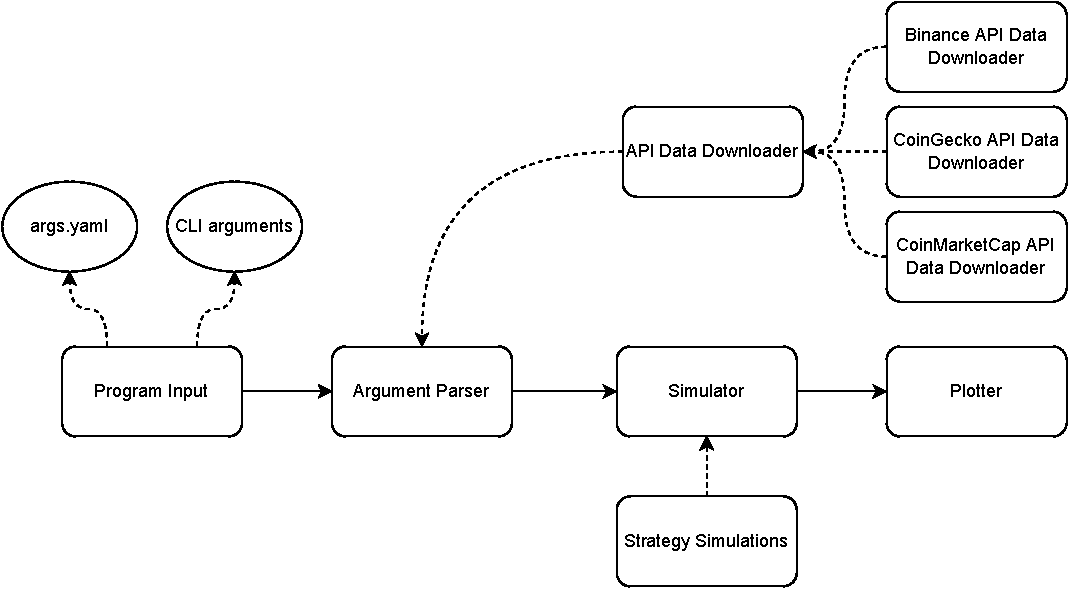
\includegraphics[width=\columnwidth]{figures/structure-diagram.pdf}
    \caption{General design structure of the backtester.}
    \label{structure-diagram}
\end{figure}

\subsection*{Strategy Class}
All strategies are derived from the base strategy abstract class. The class provides the common functions, constants and data initialization. The inherited classes usually overwrite the \texttt{execute\_step} method, which does a singular step of the strategy (1 day if the data is days apart).

One interesting strategy in particular is the StrategyMerger class that allows merging the behavior of several strategies. It basically combines the \texttt{execute\_step} of the strategies in the order they are defined.

Strategy classes with their most important attributes are shown in Figure~\ref{figure-strategy-class-diagram}. There are many prepared classes that the user can simulate with.

\begin{figure}[!t]
    \centering
    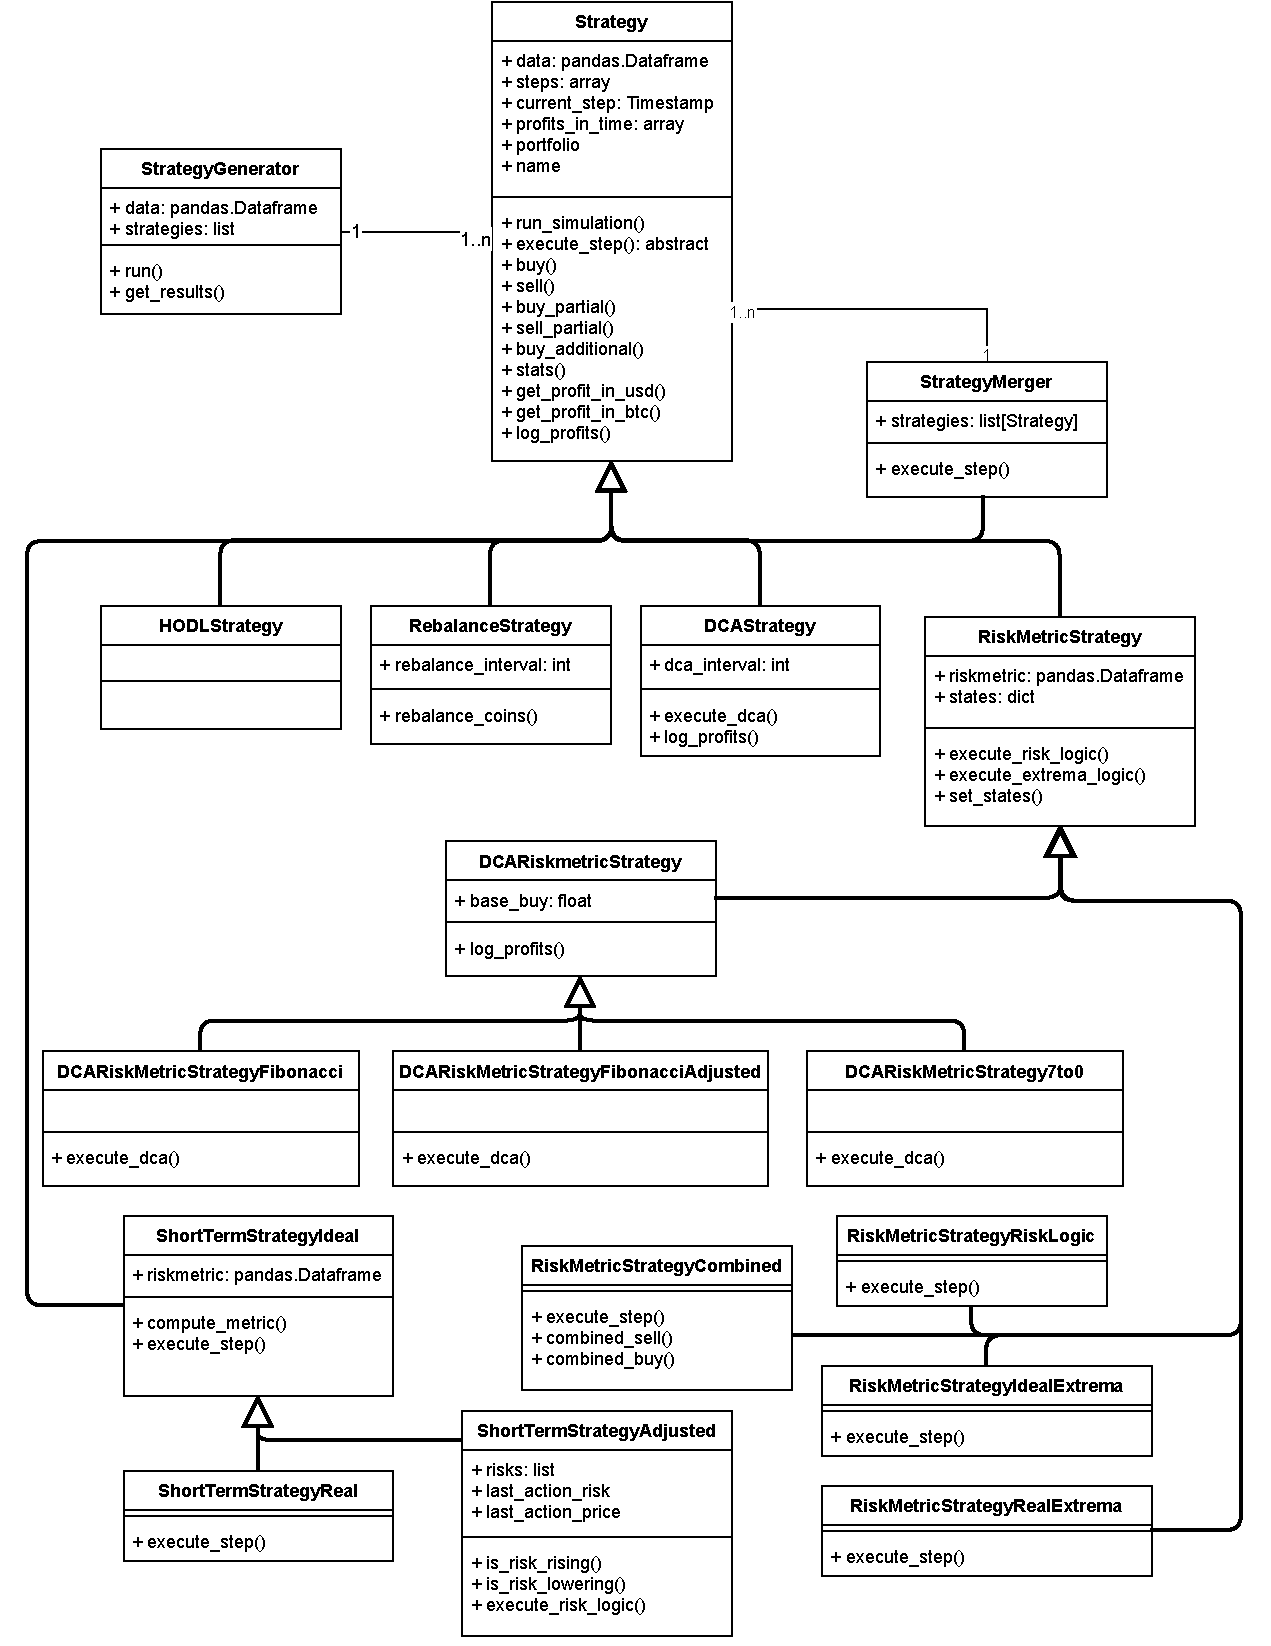
\includegraphics[width=\columnwidth]{figures/strategy-class-diagram.pdf}
    \caption{Class diagram of strategies of the backtester.}
    \label{figure-strategy-class-diagram}
\end{figure}


\section{Trading Data}
Initial trading data that was used for the experiments were initially provided by the supervisor. Due to their incompleteness and due to them being out-of-date, there was a need for more complete data.

I~designed the data fetch into a few categories. I~then researched each category and chose the best suited API provider for the thesis.

\subsection*{OHLCV Data}
I~needed OHLCV 5 minute and 1 hour data to test various strategies this way. After going through some recommendations, I~settled with Binance API\footnote{\url{https://www.binance.com/en/support/faq/c-6}} for OHLCV data since I~already had an account with them. All that is needed are public and secret API keys to make the requests.

\subsection*{Historical BTC}
One of the disadvantages of Binance API is that it only goes as far back as it started. That is to the July 2018. When calculating things like Bitcoin risk metric, it is advantageous to have earlier data available. To this end, I~used the free and public CoinGecko API~\cite{coingecko:documentation}. The \texttt{coins/market\_chart} endpoint was ideal for this use case.

Historical data have daily interval and include only the price and volume of each day, so it is not the standard OHLCV data. The data dates to the year 2013.

\subsection*{Global Metrics}
Another need due to the alternative risk metric was created for the total crypto market capitalization. This data is not present in Binance nor CoinGekco API. The perfect information was found at CoinMarketCap website\footnote{\url{https://coinmarketcap.com/charts/}}. After a bit of web scraping, I~got to the original API call\footnote{\url{https://api.coinmarketcap.com/data-api/v3/global-metrics/quotes/historical?interval=1d}}.

The data includes several useful metrics. The most important one is the total market capitalization of each day dating to year 2013. Other useful ones are 24 hour volume and bth/eth dominance for each day.

\subsection*{Implementing the Fetch}
Ideally, we would get all of our data from a single API provider. Unfortunately, I~have found no single provider that provides the needed data in the requested format.

\texttt{python-binance}\footnote{\url{https://pypi.org/project/python-binance/}} 3rd party module is used to ease the getting the data from Binance API. \texttt{pycoingecko}\footnote{\url{https://pypi.org/project/pycoingecko/}} does the same thing for the CoinGecko API. Data got from CoinMarketCap are fetched via the interface of the 3rd party module \texttt{requests}\footnote{\url{https://pypi.org/project/requests/}}

The only API that needs public and private keys is the Binance API. The keys are hidden in the \texttt{.env} file and got from the configuration library called \texttt{python-decouple}\footnote{\url{https://pypi.org/project/python-decouple/}}

\section{Data Input}
There are a few different program arguments that are needed to be specified.

Pairs are used to select the cryptocurrency pairs we want to trade. Since Binance requires both of the assets to be cryptocurrencies, we cannot select \$USD. The closest asset to it is the token that is pegged against \$USD, USDT. So if you want to choose a trading pair where the price of Bitcoin and \$USD is compared, choose BTCUSDT.

Starting and ending date do exactly as the name suggests, they define the data range in which the data is fetched. The interval argument defines the OHLCV interval between each data, it uses Binance abbreviations and there are several possible values. The values I~mostly used were 5m and 1h interval, that means that the OHLCV data fetched will be either 5 minute or 1 hour apart.

Due to a possible long list of argument values, the arguments can be saved into a file in the YAML\footnote{\url{https://yaml.org/}} format. Its schema is then validated and arguments dictionary retrieved via the \texttt{schema}\footnote{\url{https://pypi.org/project/schema/}} and \texttt{PyYAML}\footnote{\url{https://pypi.org/project/PyYAML/}} Python libraries, respectively.

Among optional arguments belongs the logging level. It defines the logging level used for logging that informs the users of filesystem manipulations, simulation progress and results, or errors and debug information. By default, it is set to level INFO.

\section{Other Auxiliary Modules}

\subsection*{Plotter}
\texttt{plotly}\footnote{\url{https://pypi.org/project/plotly/}} is used for plotting the final graphs. It works natively with the data frame data used in \texttt{pandas}.

\subsection*{Risk Metric Calculator}
Risk metric calculator is a module that is responsible for calculating risk metric. It can either work with historical Bitcoin data or total market capitalization. It defines optimizations data class that eases the work with risk metric combinations.

\subsection*{Utils}
Utils module is responsible for providing many helpful functions and defining constants that are used throughout the whole codebase. It does not have any dependencies to other modules, since that could create a cyclical import problem.

\section{Deployment and Development}
During the development of the project, code standards were enforced via various programming tools, such as linters, formatters, pre-commit and CI checks. All the selected technologies can be viewed in the repository of the project.

\subsection*{Containerization--Docker}
For ease of development and deployment, the project has been packaged into a container that can be run via the docker command. This way anyone can easily try out the program or develop it having only the required docker command installed.

Other containerization benefits include:
\begin{itemize}
    \item Runtime Environment Agnosticism
    \item Isolation from other processes
    \item Portability
    \item Ease of delivery
    \item Scalability
\end{itemize}

\subsection*{Virtual Environment}
Other option on how to develop the project is to use the Python virtual environment. \texttt{virtulenv}\footnote{\url{https://pypi.org/project/virtualenv/}} is used in the project, but other tools like \texttt{venv}\footnote{\url{https://docs.python.org/3/library/venv.html}} and \texttt{conda}\footnote{\url{https://docs.conda.io/en/latest/}} could be used.

After activating the environment and installing the required packages via \texttt{pip}. The project is ready to be run and developed. Of course, the project can be developed without ever activating the virtual environment. Conflicting Python packages and versions may cause a dependency problem, though. This way the whole project is separated from the local installation of the operating system.

\subsection*{Makefile}
Makefile is used to put a common interface for all the other commands and tools. It is recommended to use the targets from Makefile for running and developing the project. All lint, format, containerization, testing, latex translation targets are located there.

\subsection*{Testing}
Simple testing was set up using the pytest framework\footnote{\url{https://docs.pytest.org/}}. The test files can be found in the \texttt{tests} folder. The tests serve to verify the basic functionality of the implemented trading strategies, most importantly the buy and sell mechanics. The current tests cover the 65\% of the code base, the coverage can be checked by running Makefile target \texttt{coverage}.

\chapter{Adaptive Strategy Experiments}
\label{chapter-experiments}

Before we can dive into the individual adaptive strategy experiments, we need some traditional strategies that we can compare the adaptive results against. HODL and rebalance will serve as such strategies. Both are very simple to implement and highly used. That makes them the perfect candidate for this purpose.

All the graphs depicted in the Section have been produced by the implemented backtester program, proving its usefulness.

\section{Evaluation Strategy}
Before we get to the individual experiments, the main process for evaluating the experiments must be described. There are 2 caveats to this process. Firstly we need to define the strategy that tells the probability of the market going up or down, let us call it the risk metric. And secondly we need to find the optimal strategy that works with this metric---that means an algorithm that decides what to do when the metric is at such level and what to do if it is in a different level---acting as a finite state machine.

Basically, the thesis can be split into a function and a finite state machine. The function's inputs are the today's date and some kind of other data used for calculating the metric (e.g., historical price of Bitcoin). The function then calculates the risk (limited between <0,1>) for the current day and passes the value to the finite state machine. The automata then decides on what to do, taking its previous steps into the account.

\subsection*{Finite State Machine Behavior}
The most basic idea is to transfer the coins to stablecoins when the risk is near the high boundary, and transfer back to coins when it is again nearing the lower boundary. Alternatively, when using the DCA (dollar cost averaging) strategy (described in Section~\ref{section-dca}, we do not invest when the risk is high and invest more money when the risk is low.

\subsection*{Evaluation Variables}
When looking at the evaluation, we need to keep in mind the variables that can influence the results greatly. Firstly, the chosen cryptocurrencies may differ quite a lot, and choosing different quantity of them influences the results, too. The other obvious variable is the date range. During evaluation, we will also try to look at the ranges that experienced only bull or bear market, not just the long data ranges. Finally, the data interval---as in 5m or 1d---may influence the data.

Some DCA portfolio can look like this:
\begin{itemize}
    \item $Risk \ge  0.7$: Do not invest.
    \item $0.6 \le Risk < 0.7$: Invest sum x1.
    \item $0.5 \le Risk < 0.6$: Invest sum x2.
    \item $0.4 \le Risk < 0.5$: Invest sum x3.
    \item $0.3 \le Risk < 0.4$: Invest sum x4.
    \item $0.2 \le Risk < 0.3$: Invest sum x5.
    \item $0.1 \le Risk < 0.2$: Invest sum x6.
    \item $Risk < 0.1$: Invest sum x7.
\end{itemize}

Coin to stablecoin ratios can look like this:
\begin{itemize}
    \item $Risk \ge  0.7$: All capital is converted to stablecoins.
    \item $0.6 \le Risk < 0.7$: 60\% converted.
    \item $0.5 \le Risk < 0.6$: 40\% converted.
    \item $0.4 \le Risk < 0.5$: 20\% converted.
    \item $0.3 \le Risk < 0.4$: Capital is in coins only.
    \item $0.2 \le Risk < 0.3$: Capital is in coins only.
    \item $0.1 \le Risk < 0.2$: Capital is in coins only.
    \item $Risk < 0.1$: Capital is in coins only.
\end{itemize}


\subsection*{Used Datasets}
We will be testing with a few portfolios. Portfolios usually start with the base value of that day's Bitcoin price. Alternatively, when using multiple coins, some base value like \$1,000 is used. Most strategy implementations are demonstrated using Bitcoin. It is much easier to see the simulation results on 1 cryptocurrency at the start. And additionally, it is the main driver behind a few strategies.

Later, a portfolio consisting of many coins is used to see how the strategy adapts to the changed scenario.


\subsection*{Benchmark Strategies}
Our benchmark strategies are going to be HODL and periodic Rebalance. Periodic rebalance is going to be set to 1 day or 5 minute interval, depending on the data interval. If the adaptive strategy outperforms the mentioned strategies, it has a good potential to be a good strategy. HODL and rebalance is often used by starting investors, so a strategy outperforming these, is a step in a good direction.

Performance of the strategies against Bitcoin and Ethereum portfolio can be seen in Figure~\ref{figure-benchmark}, in logarithmic scale. We can see that the periodic rebalance interval matters, although only a bit. We will use the shortest interval, as suggested by the assumptions in Section~\ref{rebalance-assumptions}.

\begin{figure}[!t]
    \centering
    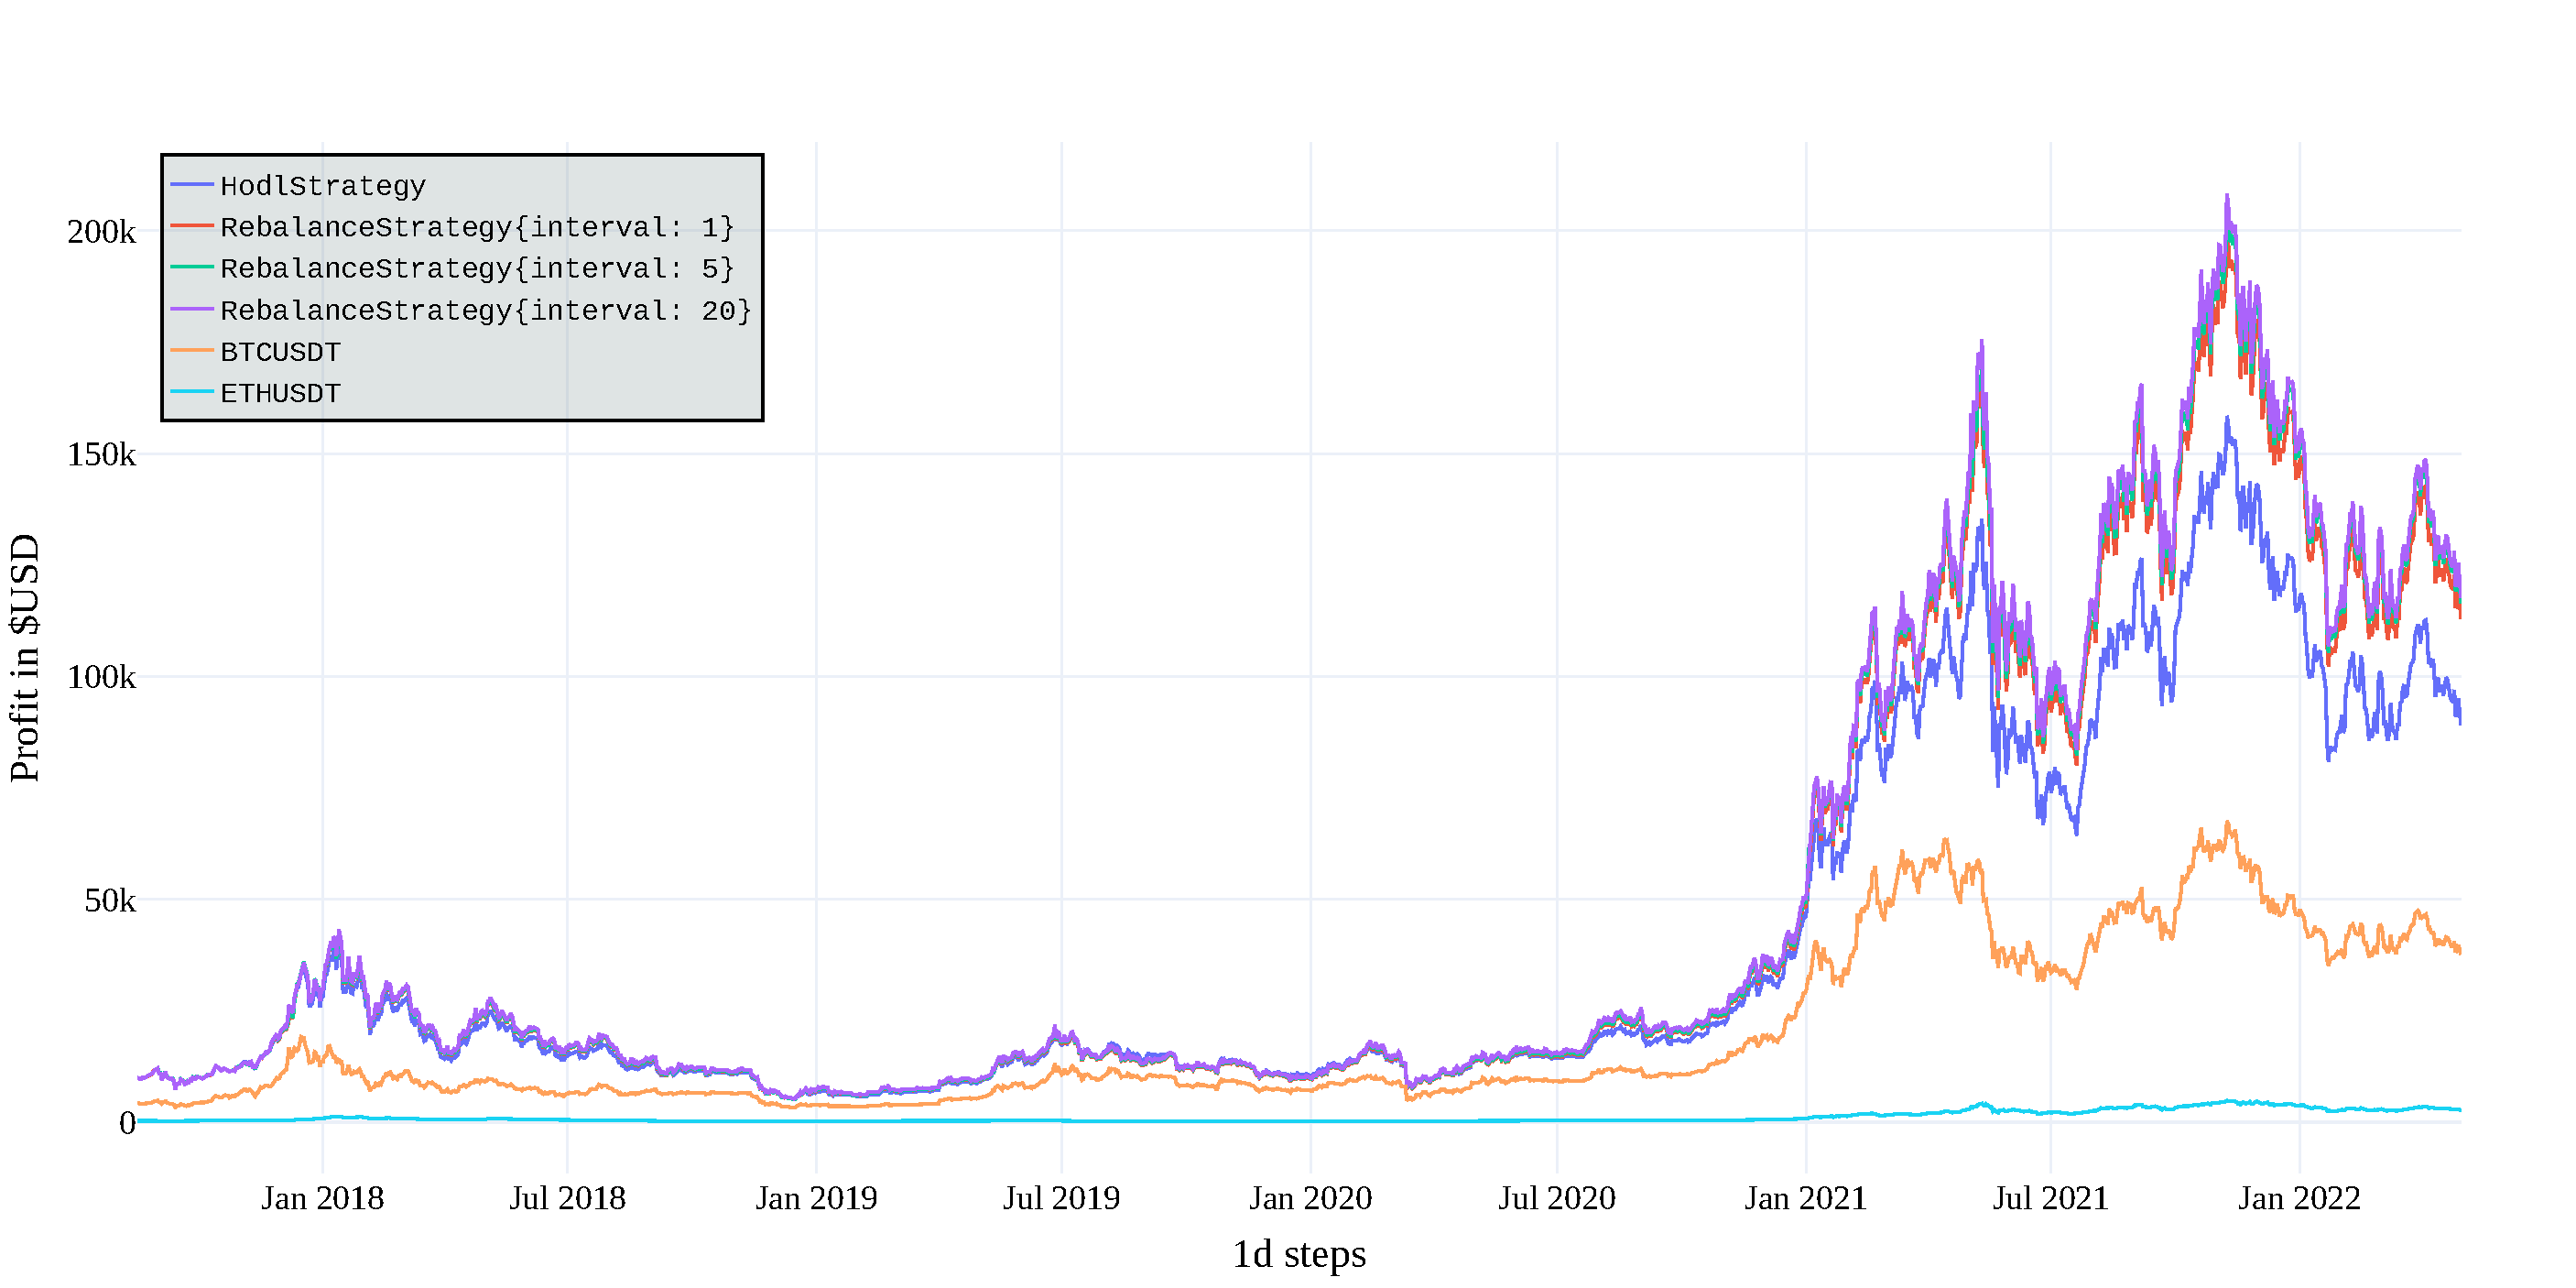
\includegraphics[width=\columnwidth]{figures/benchmark.pdf}
    \caption{HODL and rebalance strategies' performance against the Bitcoin and Ethereum portfolio.}
    \label{figure-benchmark}
\end{figure}


\section{Implementation of Strategies---Risk Metric}
\label{section-strategies}
\emph{Bitcoin risk metric} term was most probably coined and invented by Benjamin Cowen on his YouTube channel~\cite{youtube:cowen-yt-channel}, or at least it is mostly associated with his figure. It is an algorithm that prescribes a certain risk value, between 0 and 1, to each day of Bitcoin price. It takes into account the maximum value that has already occurred so far in the history. This strategy is often favorable by DCA. Depending on the risk scale, you either invest more if the risk is lower and invest less (or not at all) if the risk is high. The metric oscillates between highs and lows. There have been 5 high points of the metric since the year 2011.

Unfortunately, Benjamin Cowen does not have his risk metric calculation formula publicly available. In a past video~\cite{youtube:cowen-moving-average}, he hinted that moving averages are used for the computation. Specifically, when you take 50 day moving average, and you divide it by 50-week moving average. That is the first value used.

\subsection*{Testing Out the 50 Week / 50 Days}
\label{subsection-50week50days}
The formula becomes:
$$risk = \frac{\mathit{SMA}_{50 days}}{\mathit{SMA}_{50 weeks}}$$

The results look quite similar to the metrics used by Benjamin Cowen. So far it is quite the approximation, but it seems to work nicely. For the reasons of the thesis, color-coded graph has been implemented. It shows the value of Bitcoin in time with a color bar on top of it---the redder it is, the higher the risk, and vice versa.

Here are the results projected on historical price of Bitcoin. Results are shown in Figures~\ref{figure-50week-scale} and~\ref{figure-50week-colorcoded} as 0-1 scale and color-coded graph respectively. As can be seen, the metric's beginning does not make much sense. It does well during the December 2017 peak. During the later peaks it performs okay, but the risk is not as high as it should be during the peak of April 2021. This tells us that we should not only look at the overall risk, but probably also at how quickly the risk changes.

\begin{figure}[!t]
    \centering
    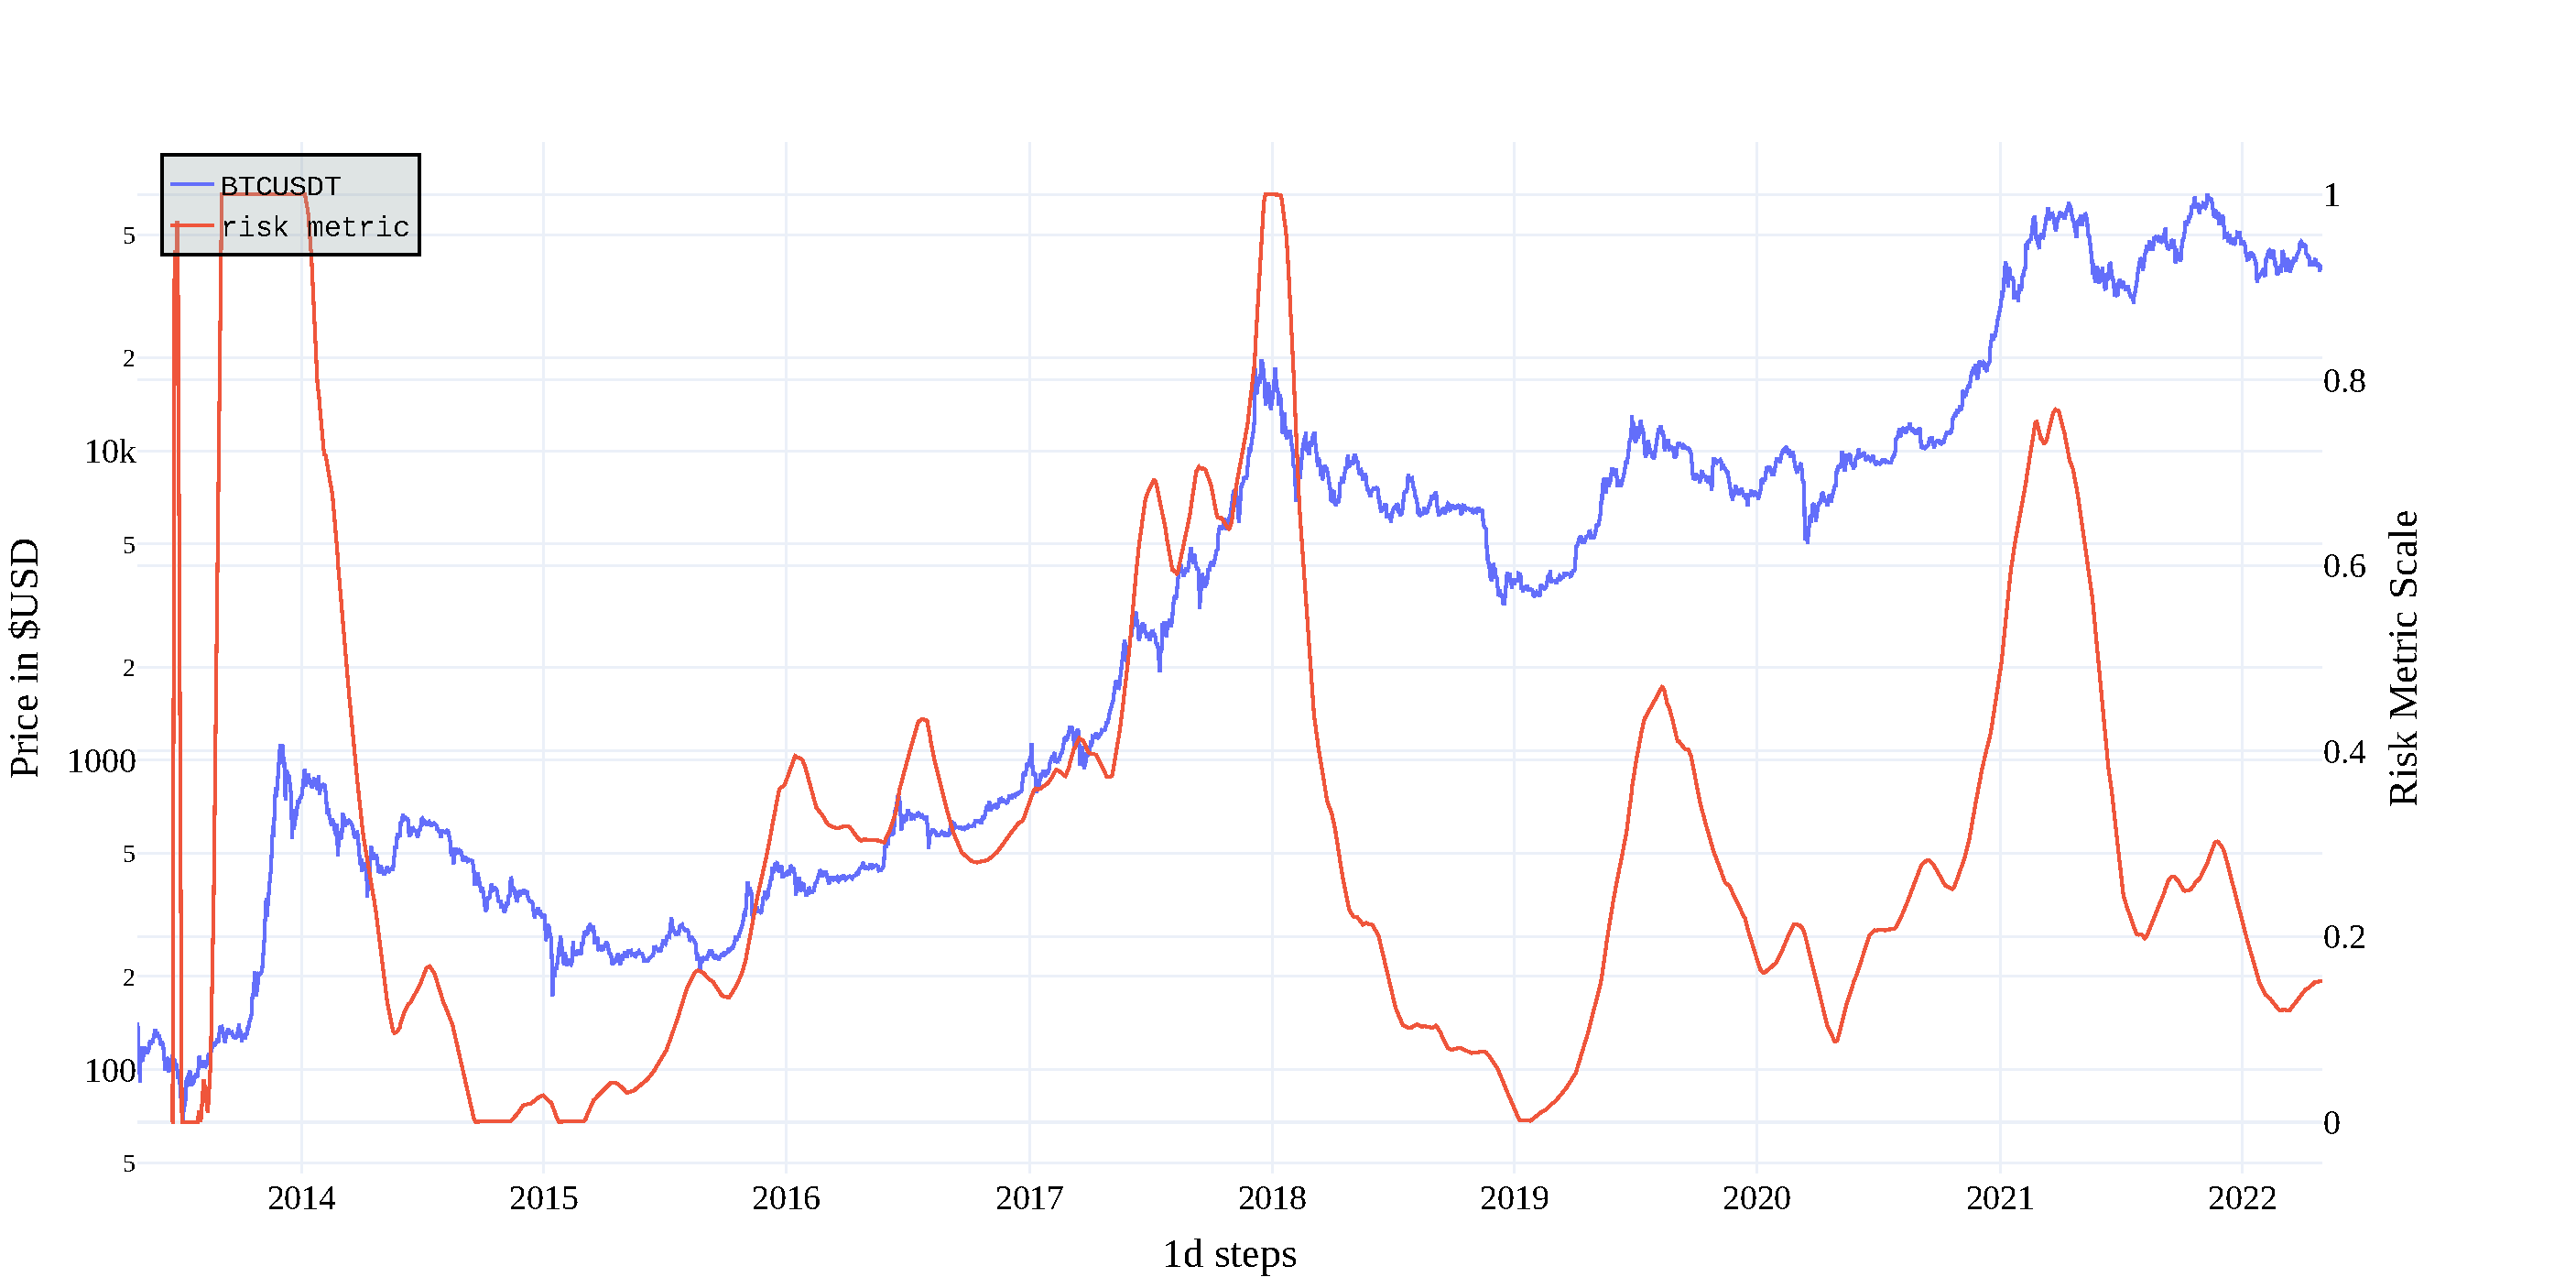
\includegraphics[width=\columnwidth]{figures/50week-scale.pdf}
    \caption{Historical Price (logarithmic) of Bitcoin with Risk Metric Scale.}
    \label{figure-50week-scale}
\end{figure}

\begin{figure}[!t]
    \centering
    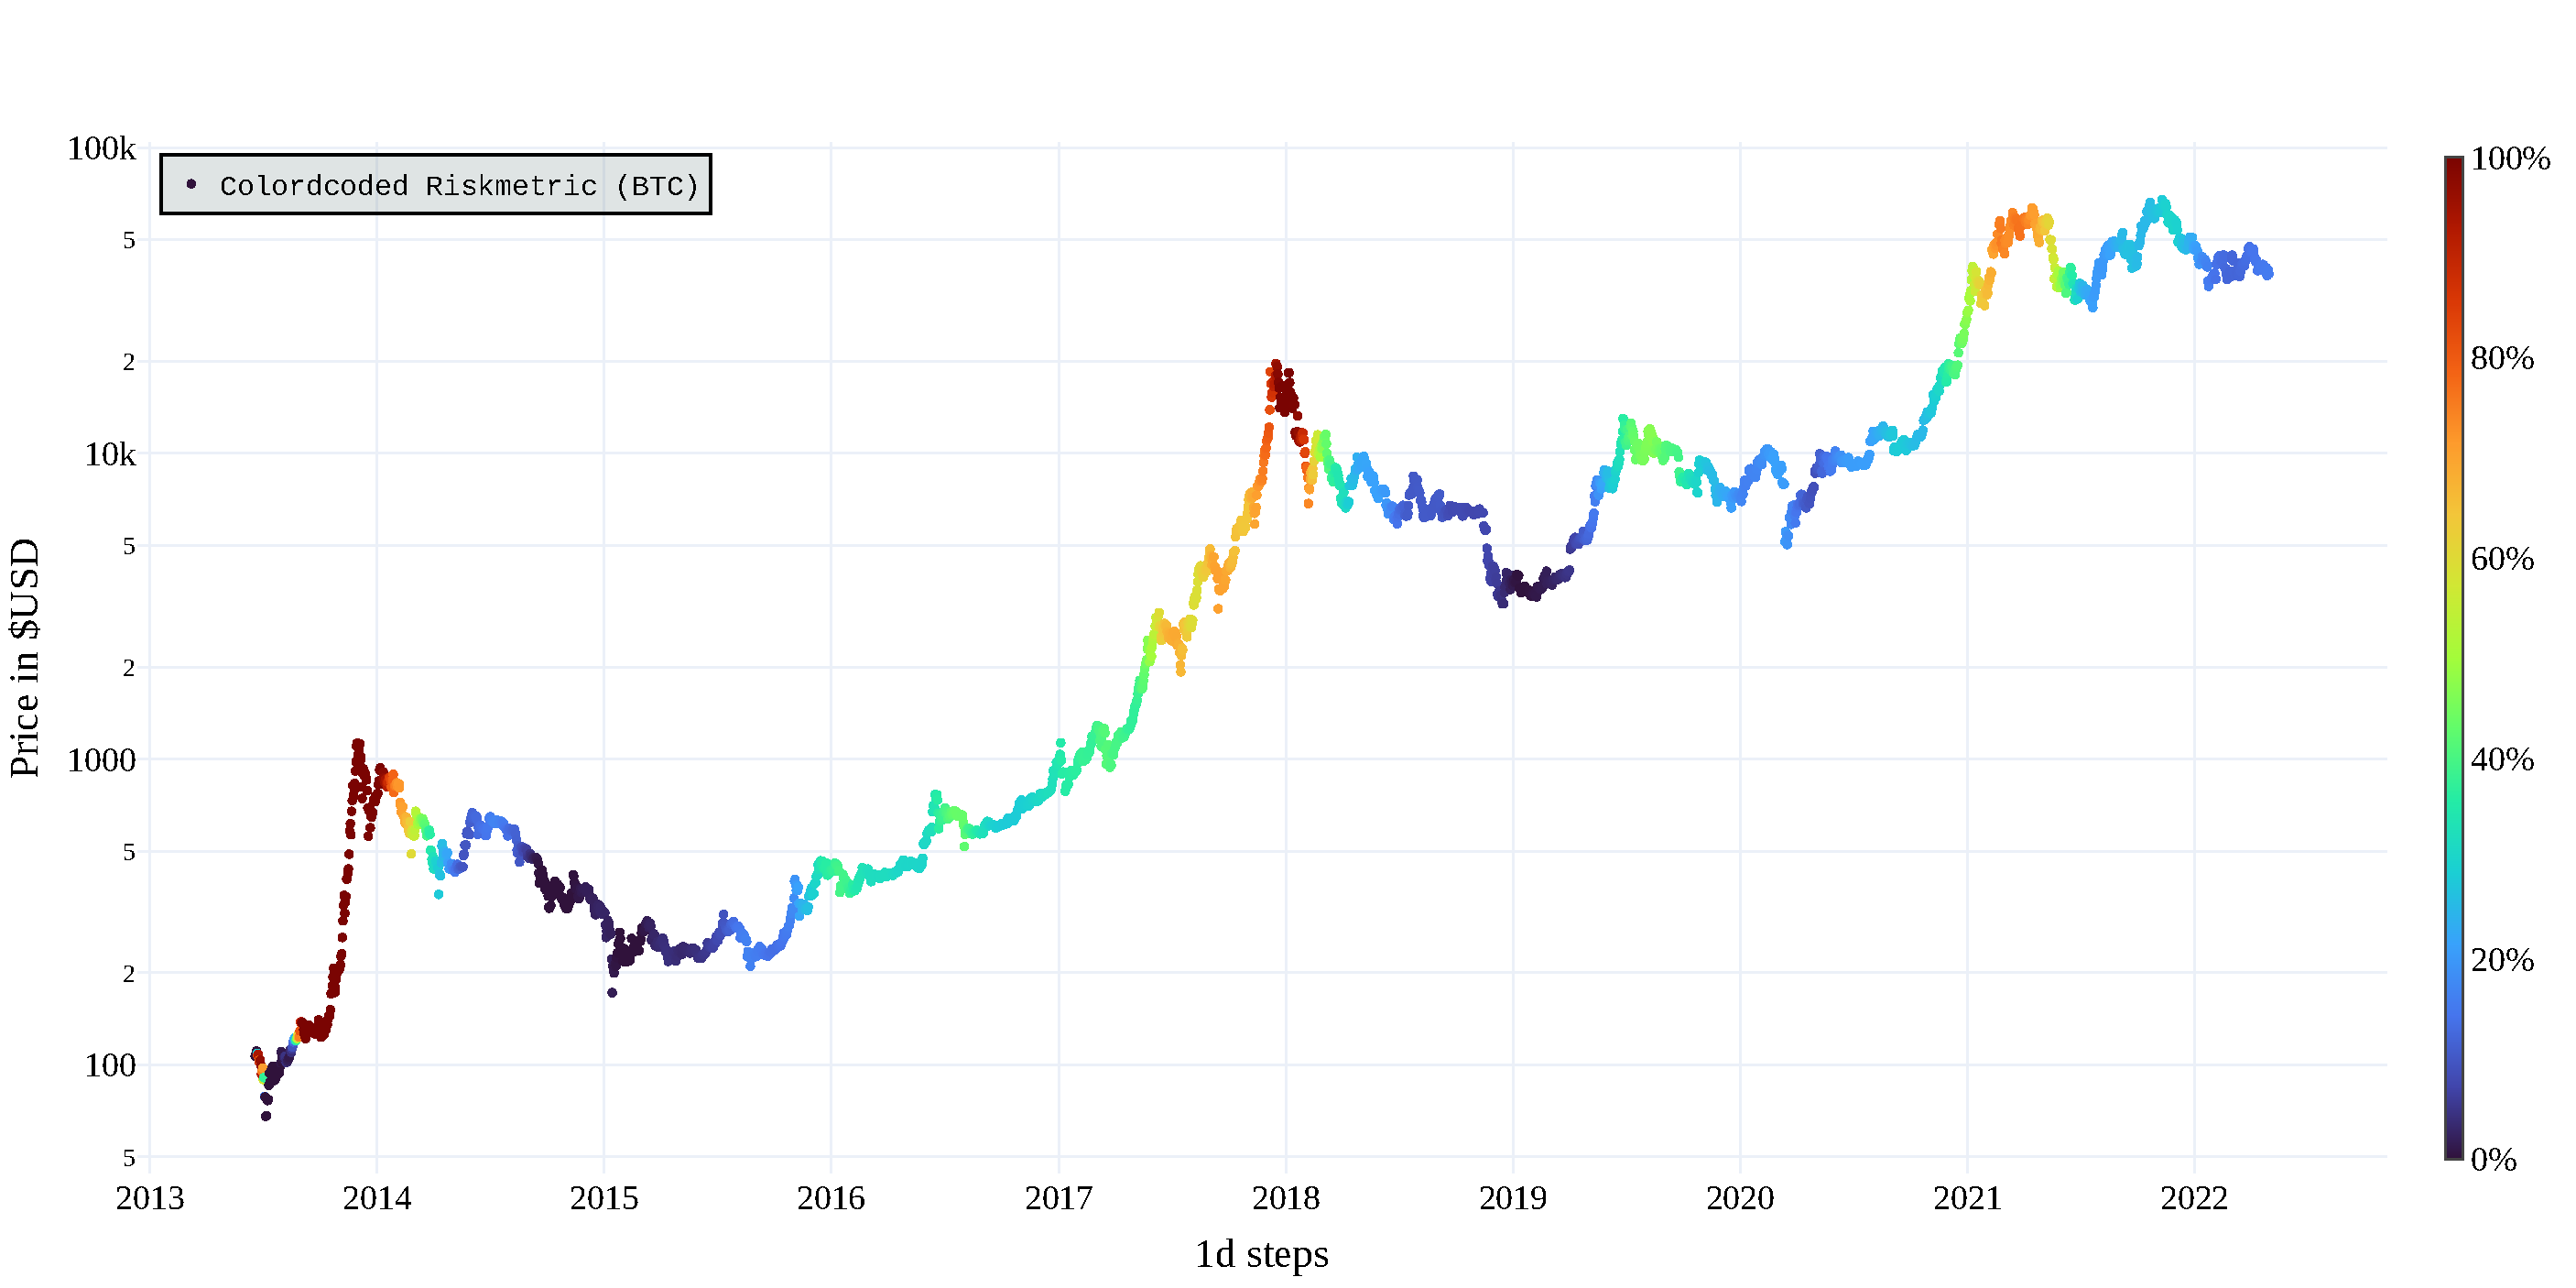
\includegraphics[width=\columnwidth]{figures/50week-colorcoded.pdf}
    \caption{Color-coded Risk Metric, logarithmic scale.}
    \label{figure-50week-colorcoded}
\end{figure}

\subsection*{Optimizing for Diminishing Returns}
\label{subsection-dimreturns}
What are diminishing returns? It is a theory in economics that predicts that after an optimal capacity level is reached, adding additional factor of production will result in smaller increase in output~\cite{investopedia:diminishing-returns}.

When we apply to Bitcoin, it means that the price growth is slowing, its returns are diminishing over time. It is supported by the fact that moving the price from 0.1\$ to 1\$ was relatively easy, but moving the price from 1000\$ to 10000\$ was significantly more difficult, requiring much more capital, even though the relative profit in percentages stays the same~\cite{bitcoin-diminishing-returns}. This would imply that expected returns of all HODLers diminish every time, making shorter-term HODLers more promising. This paragraph has been inspired by the source~\cite{bitcoin-diminishing-returns}.

The formula used by the diminishing returns has been inspired by this article~\cite{bitcoin-diminishing-returns-formula}. General formula used:
$$price = 10^{(a + b \log_{10}(d))}$$

with a = -17.01593313 and the slope b = 5.84509376 with d the number of days since 2009 Jan 12, first ever recorded Bitcoin exchange.

The expected price of Bitcoin, according to the formula above, can be seen in Figure~\ref{figure-dim-riskmetric}. The formula tells us that we should optimize for diminishing returns, but not only that. The equation itself can be used to serve as a metric. If the price is above the expected threshold, the investor should be cautious. When it is below, the investor can act more bullishly.

For now, let us only optimize the risk metric we have so far implemented. Optimizing for diminishing returns in this sense means that the risk should be higher for the later dates, even though the moving averages have the same values. The result of moving averages will be multiplied by some constant that is computed by the number of days that have passed since the year 2009. The previous formula becomes:

$$risk = \frac{\mathit{SMA}_{50 days}}{\mathit{SMA}_{50 weeks}} * \log_{10}(d)$$

The $\log$ part could be further tweaked with, but I~have found that it works quite nicely. In Figure~\ref{figure-dim-riskmetric} you can see the optimized risk metric against the original.

\begin{figure}[!t]
    \centering
    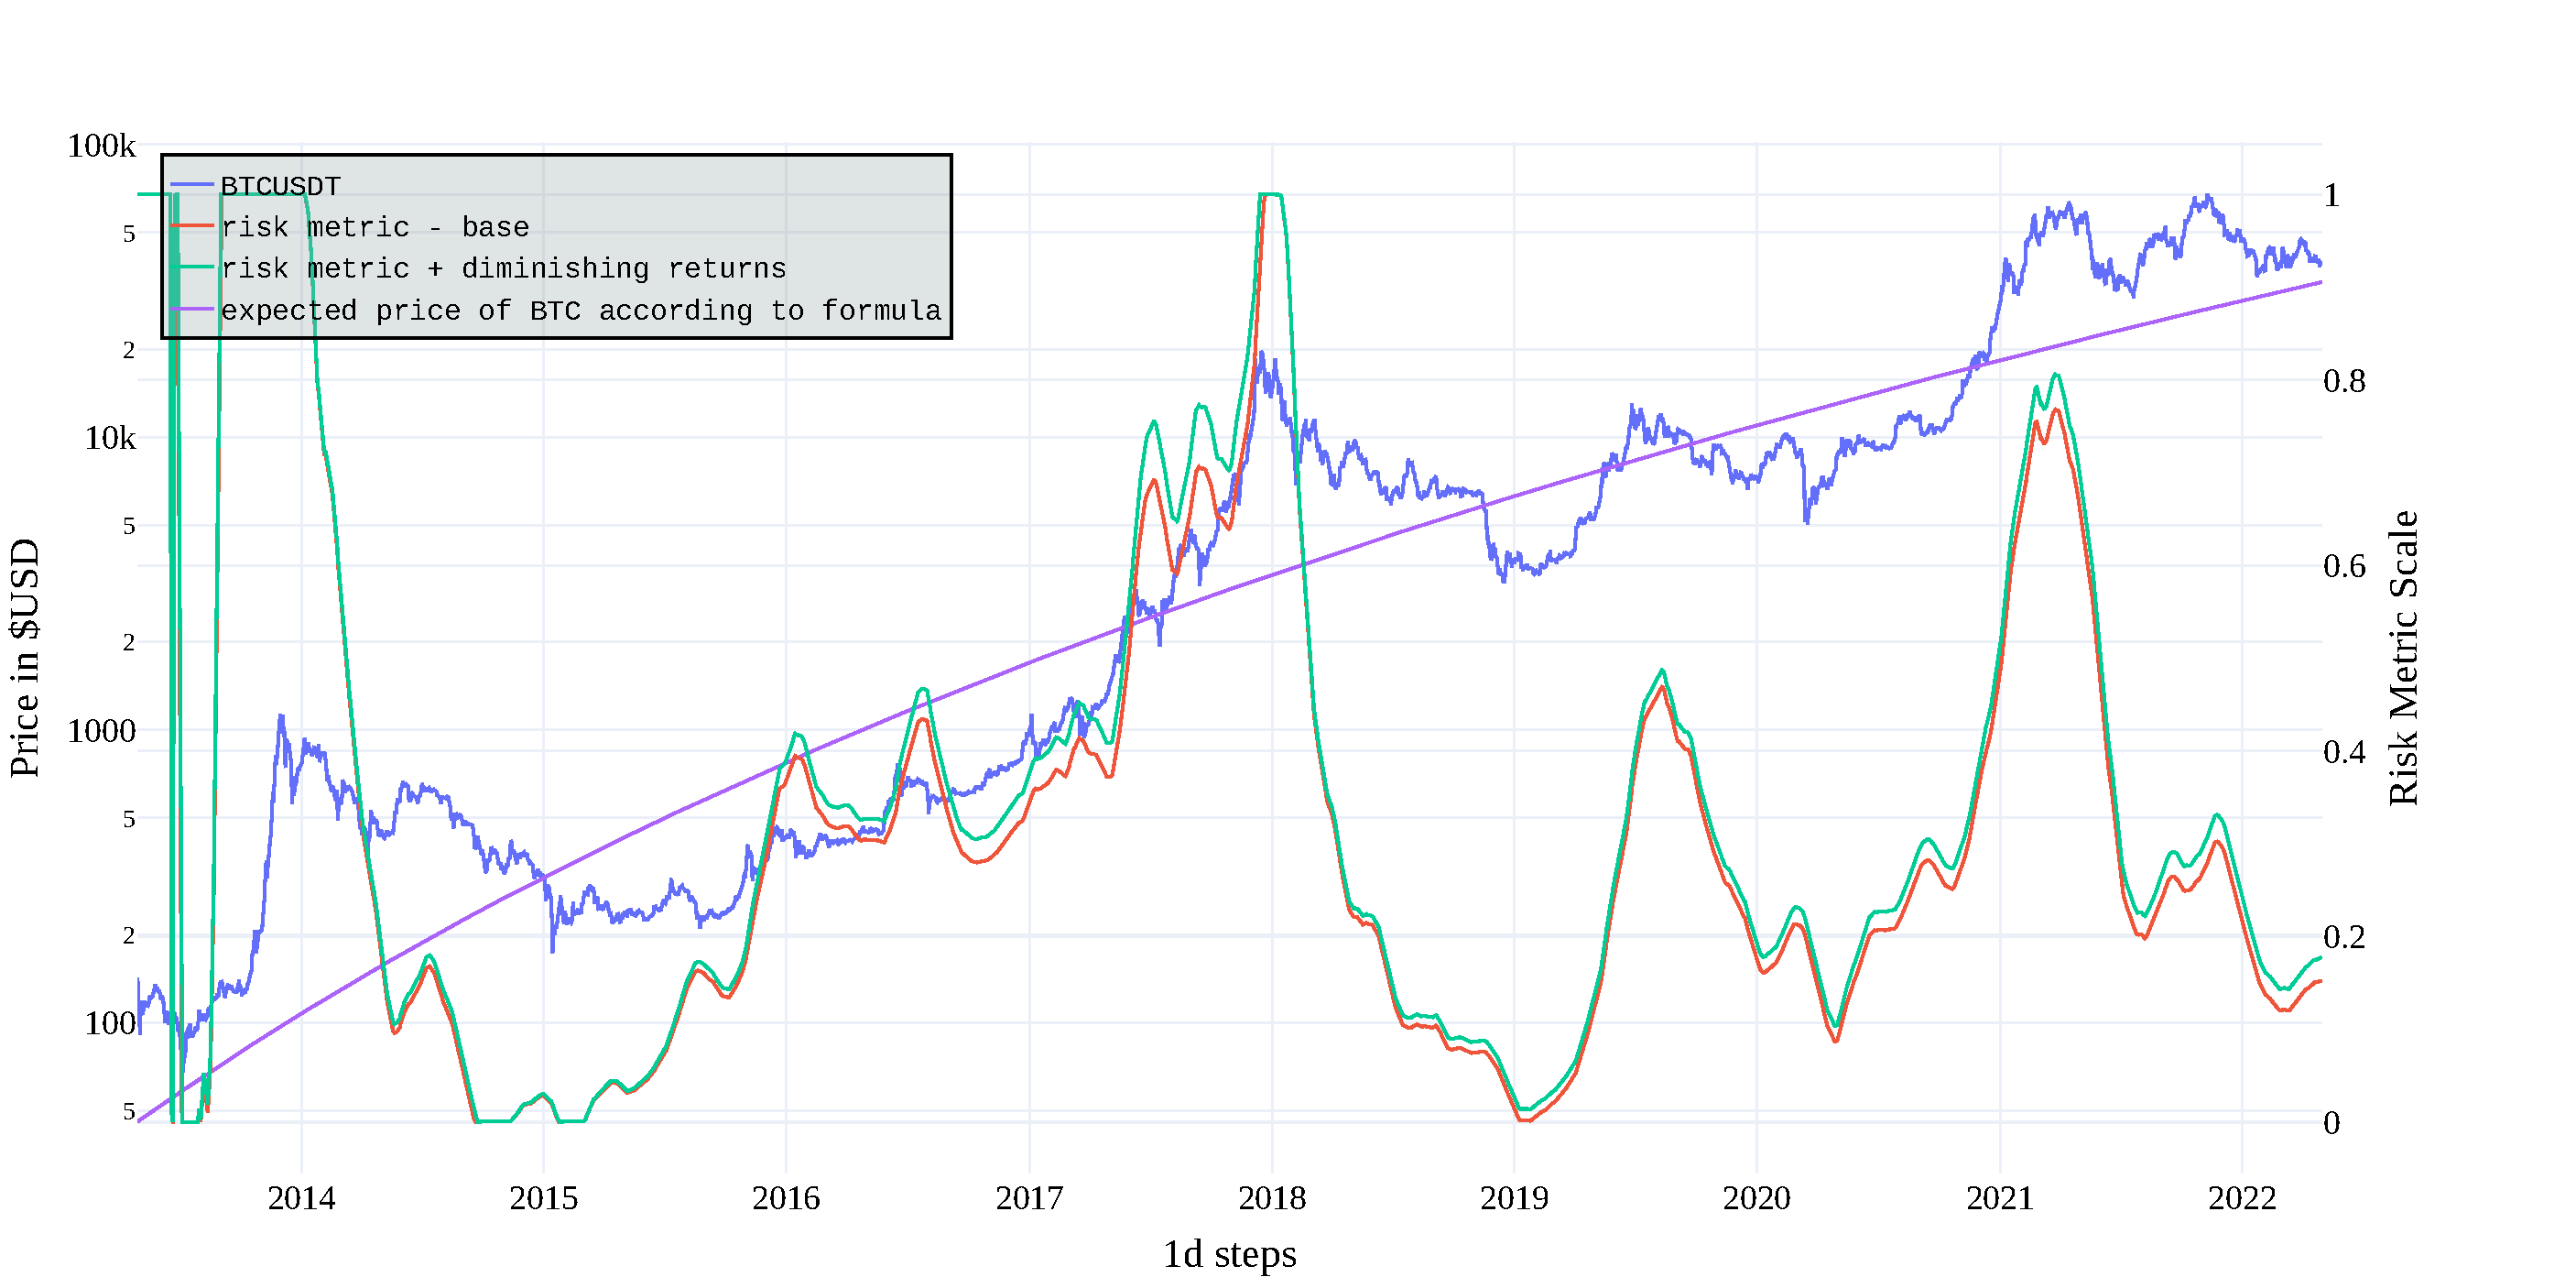
\includegraphics[width=\columnwidth]{figures/riskmetric-dim-returns.pdf}
    \caption{Comparison of the diminishing returns optimization against the standard version, an expected price of Bitcoin according to the aforementioned formula.}
    \label{figure-dim-riskmetric}
\end{figure}

\subsection*{Using Total Market Capitalization Data}
\label{subsection-marketcap}
Other thing considered is using the total market capitalization data instead of the historical price for Bitcoin. This metric makes sense when using more types of cryptocurrencies than just Bitcoin. All calculations and formulas stay the same, the only that changes is the data used---switching Bitcoin data for total market capitalization.

In Figure~\ref{figure-total-marketcap-riskmetric}, comparison of the previous findings with the Bitcoin risk metric can be seen. The metrics are quite similar, the bigger difference is that the total market capitalization metric gives more importance to the jump of July 2017. The diminishing returns optimization alter the metrics, but no other change is observed.

\begin{figure}[!t]
    \centering
    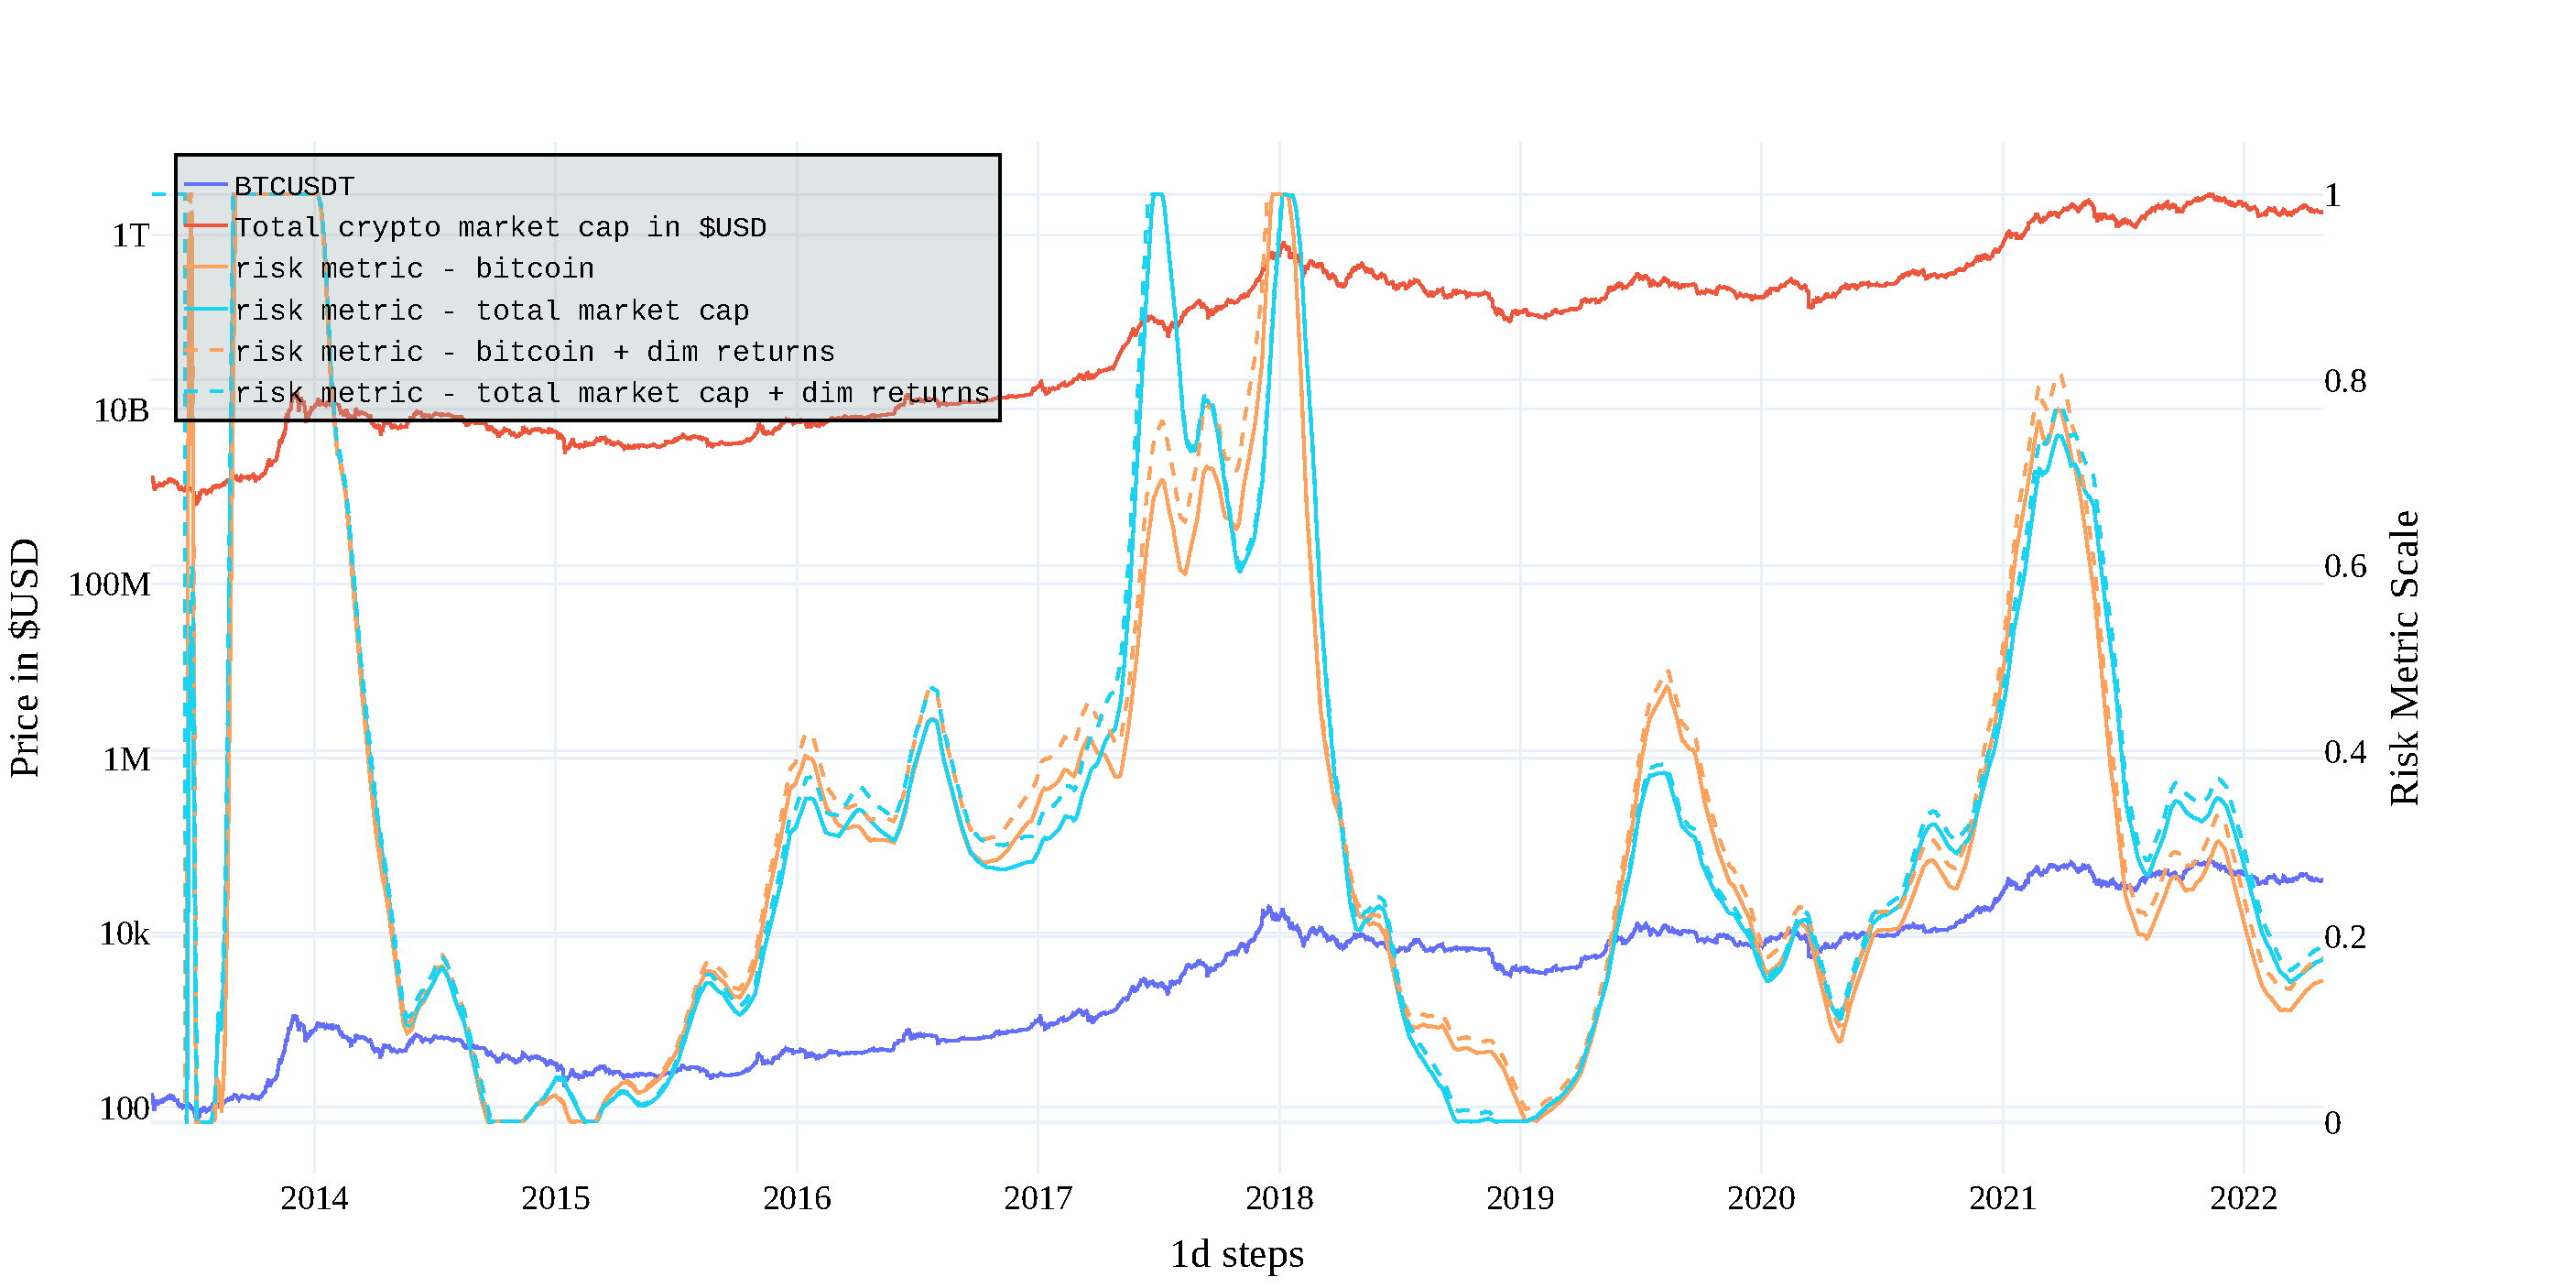
\includegraphics[width=\columnwidth]{figures/totalmarketcap-metric.pdf}
    \caption{Comparison of Bitcoin data use against total market capitalization data for the risk metric. Diminishing returns optimization is represented by dash lines.}
    \label{figure-total-marketcap-riskmetric}
\end{figure}


\subsection*{Correlation With 24h Volume Data}
\label{subsection-24hvolume-correlation}
When using a strategy like the risk metric we have implemented, we are betting on one horse, so to speak. Some unexpected turn can make us lose a lot of money. That is why it is sometimes more efficient to use a correlation with a different strategy to make the original strategy less error-prone. That is the motivation for this Section.

Correlation with the volume in \$USD traded in one day has been chosen for our strategy. It is a sensible metric. When more people trade the asset, the price can be expected to fluctuate a lot---usually up---and vice versa.

The data correlation between the two series is approximately $0.73$, with $1$ being the best positive correlation. The computed correlation is not perfect, but it gives us a good basis to work upon. Comparison can be seen in Figures~\ref{figure-24volume-ols},~\ref{figure-24volume-lin} and~\ref{figure-24volume-log}.

\begin{figure}[!t]
    \centering
    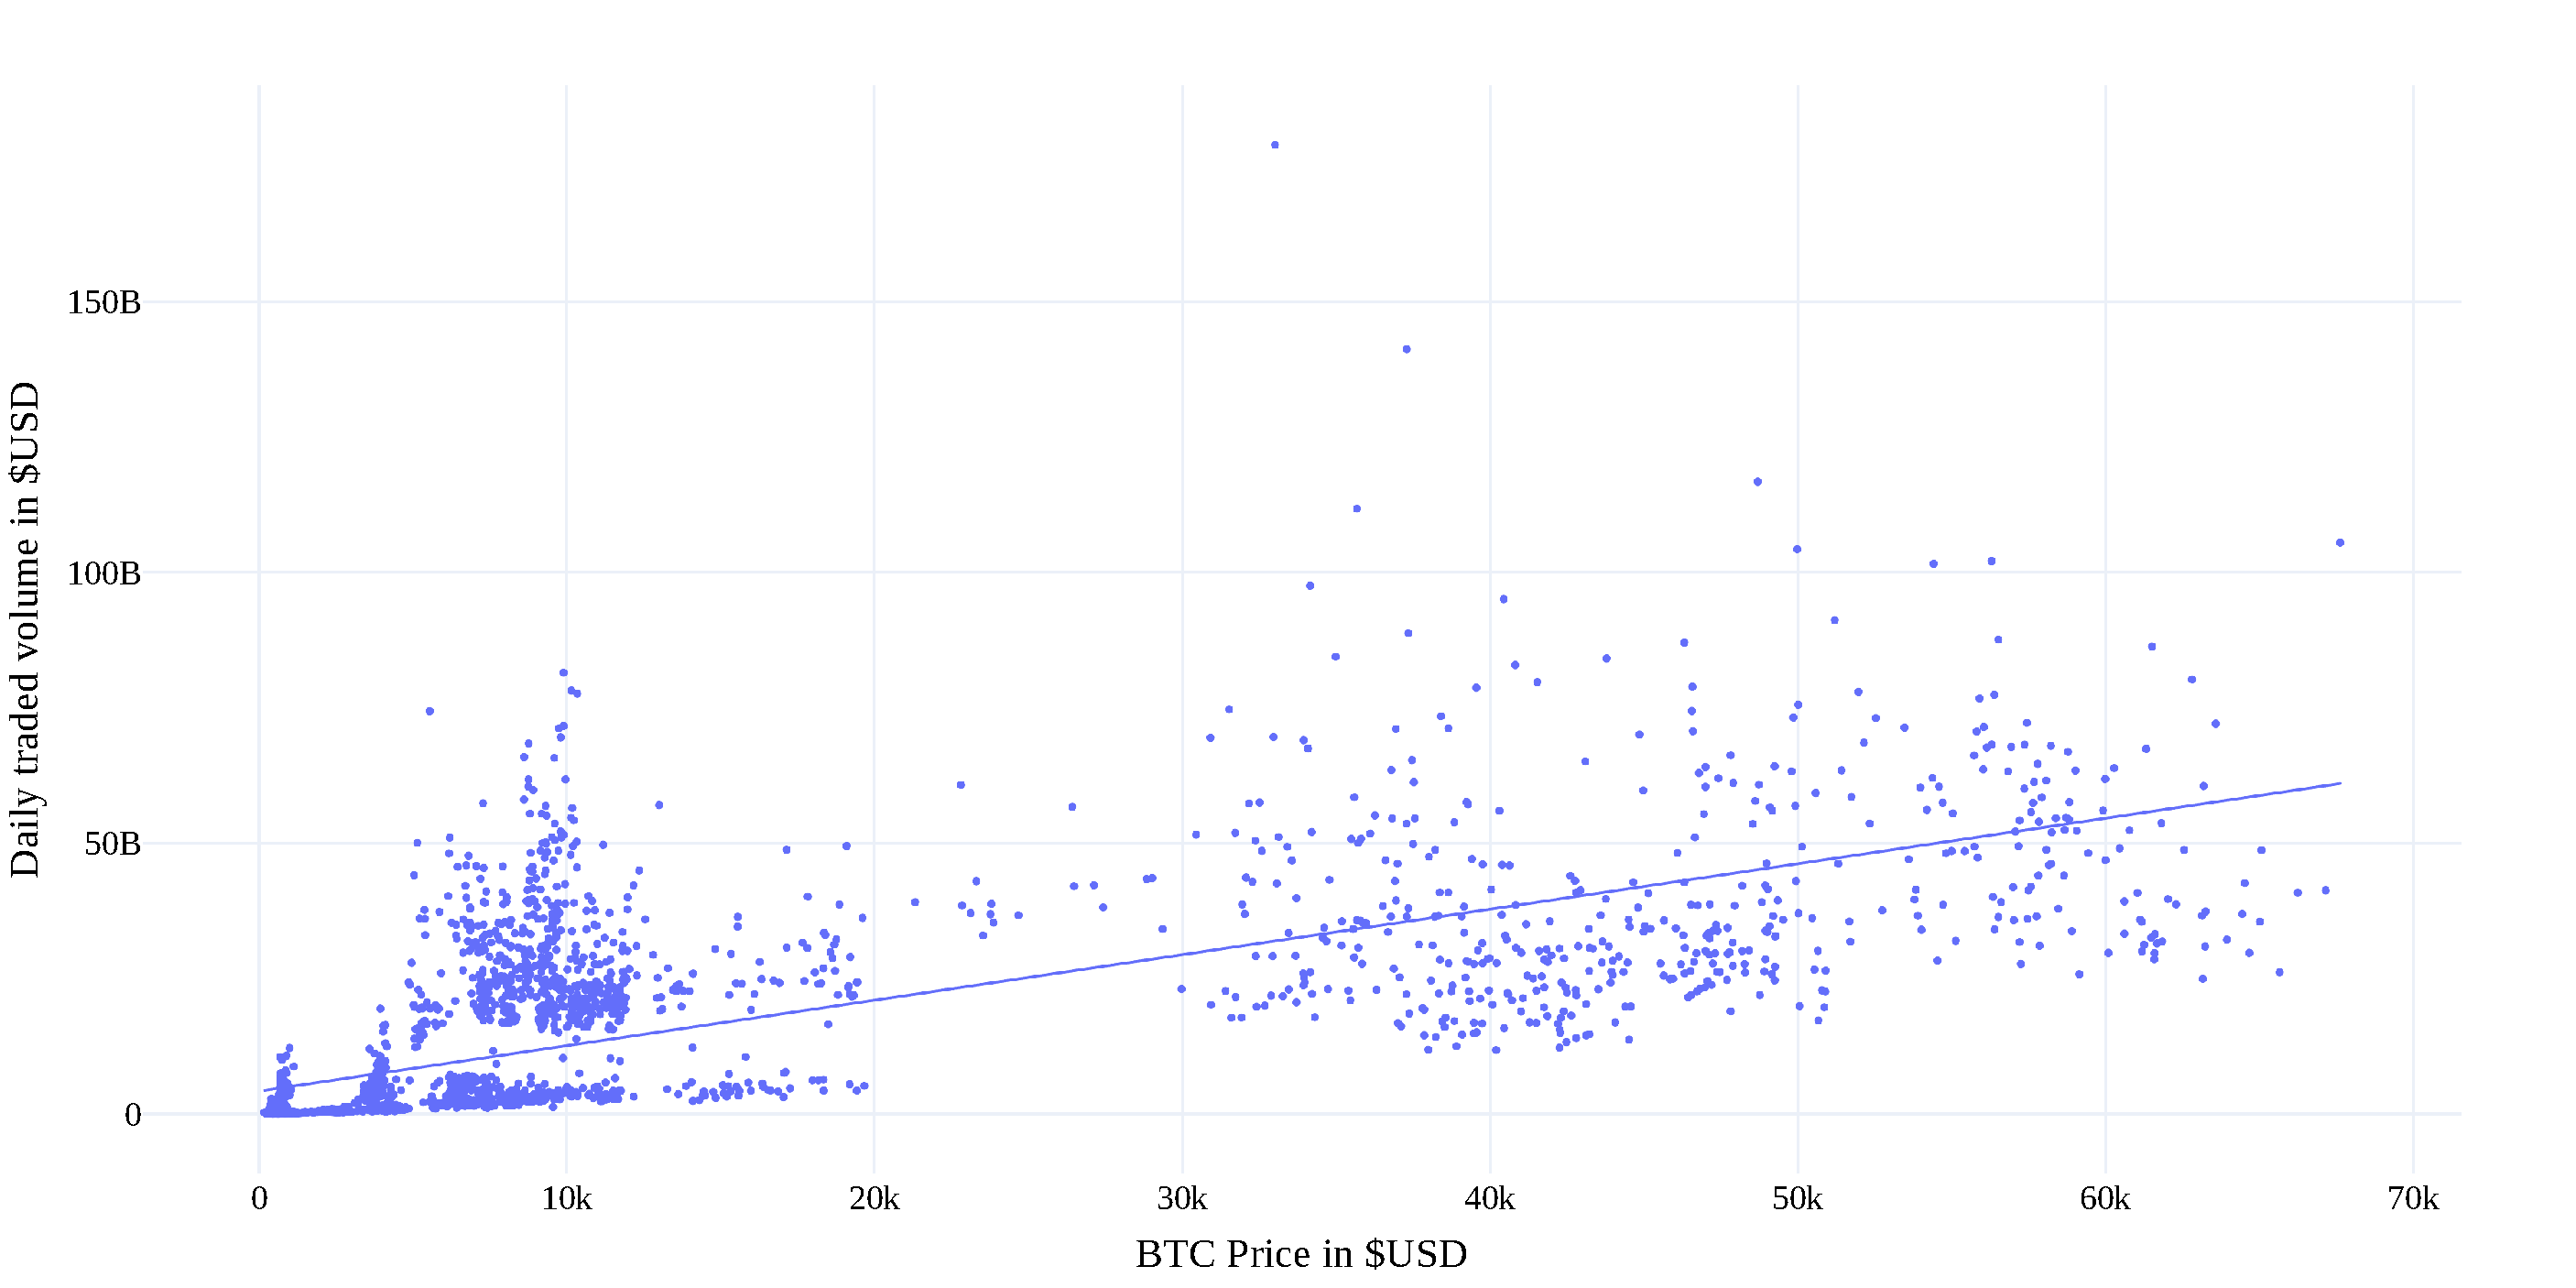
\includegraphics[width=\columnwidth]{figures/24volume-ols.pdf}
    \caption{Ordinary Least Squares method~\cite{wikipedia:ols} visualizing the correlation.}
    \label{figure-24volume-ols}
\end{figure}

\begin{figure}[!t]
    \centering
    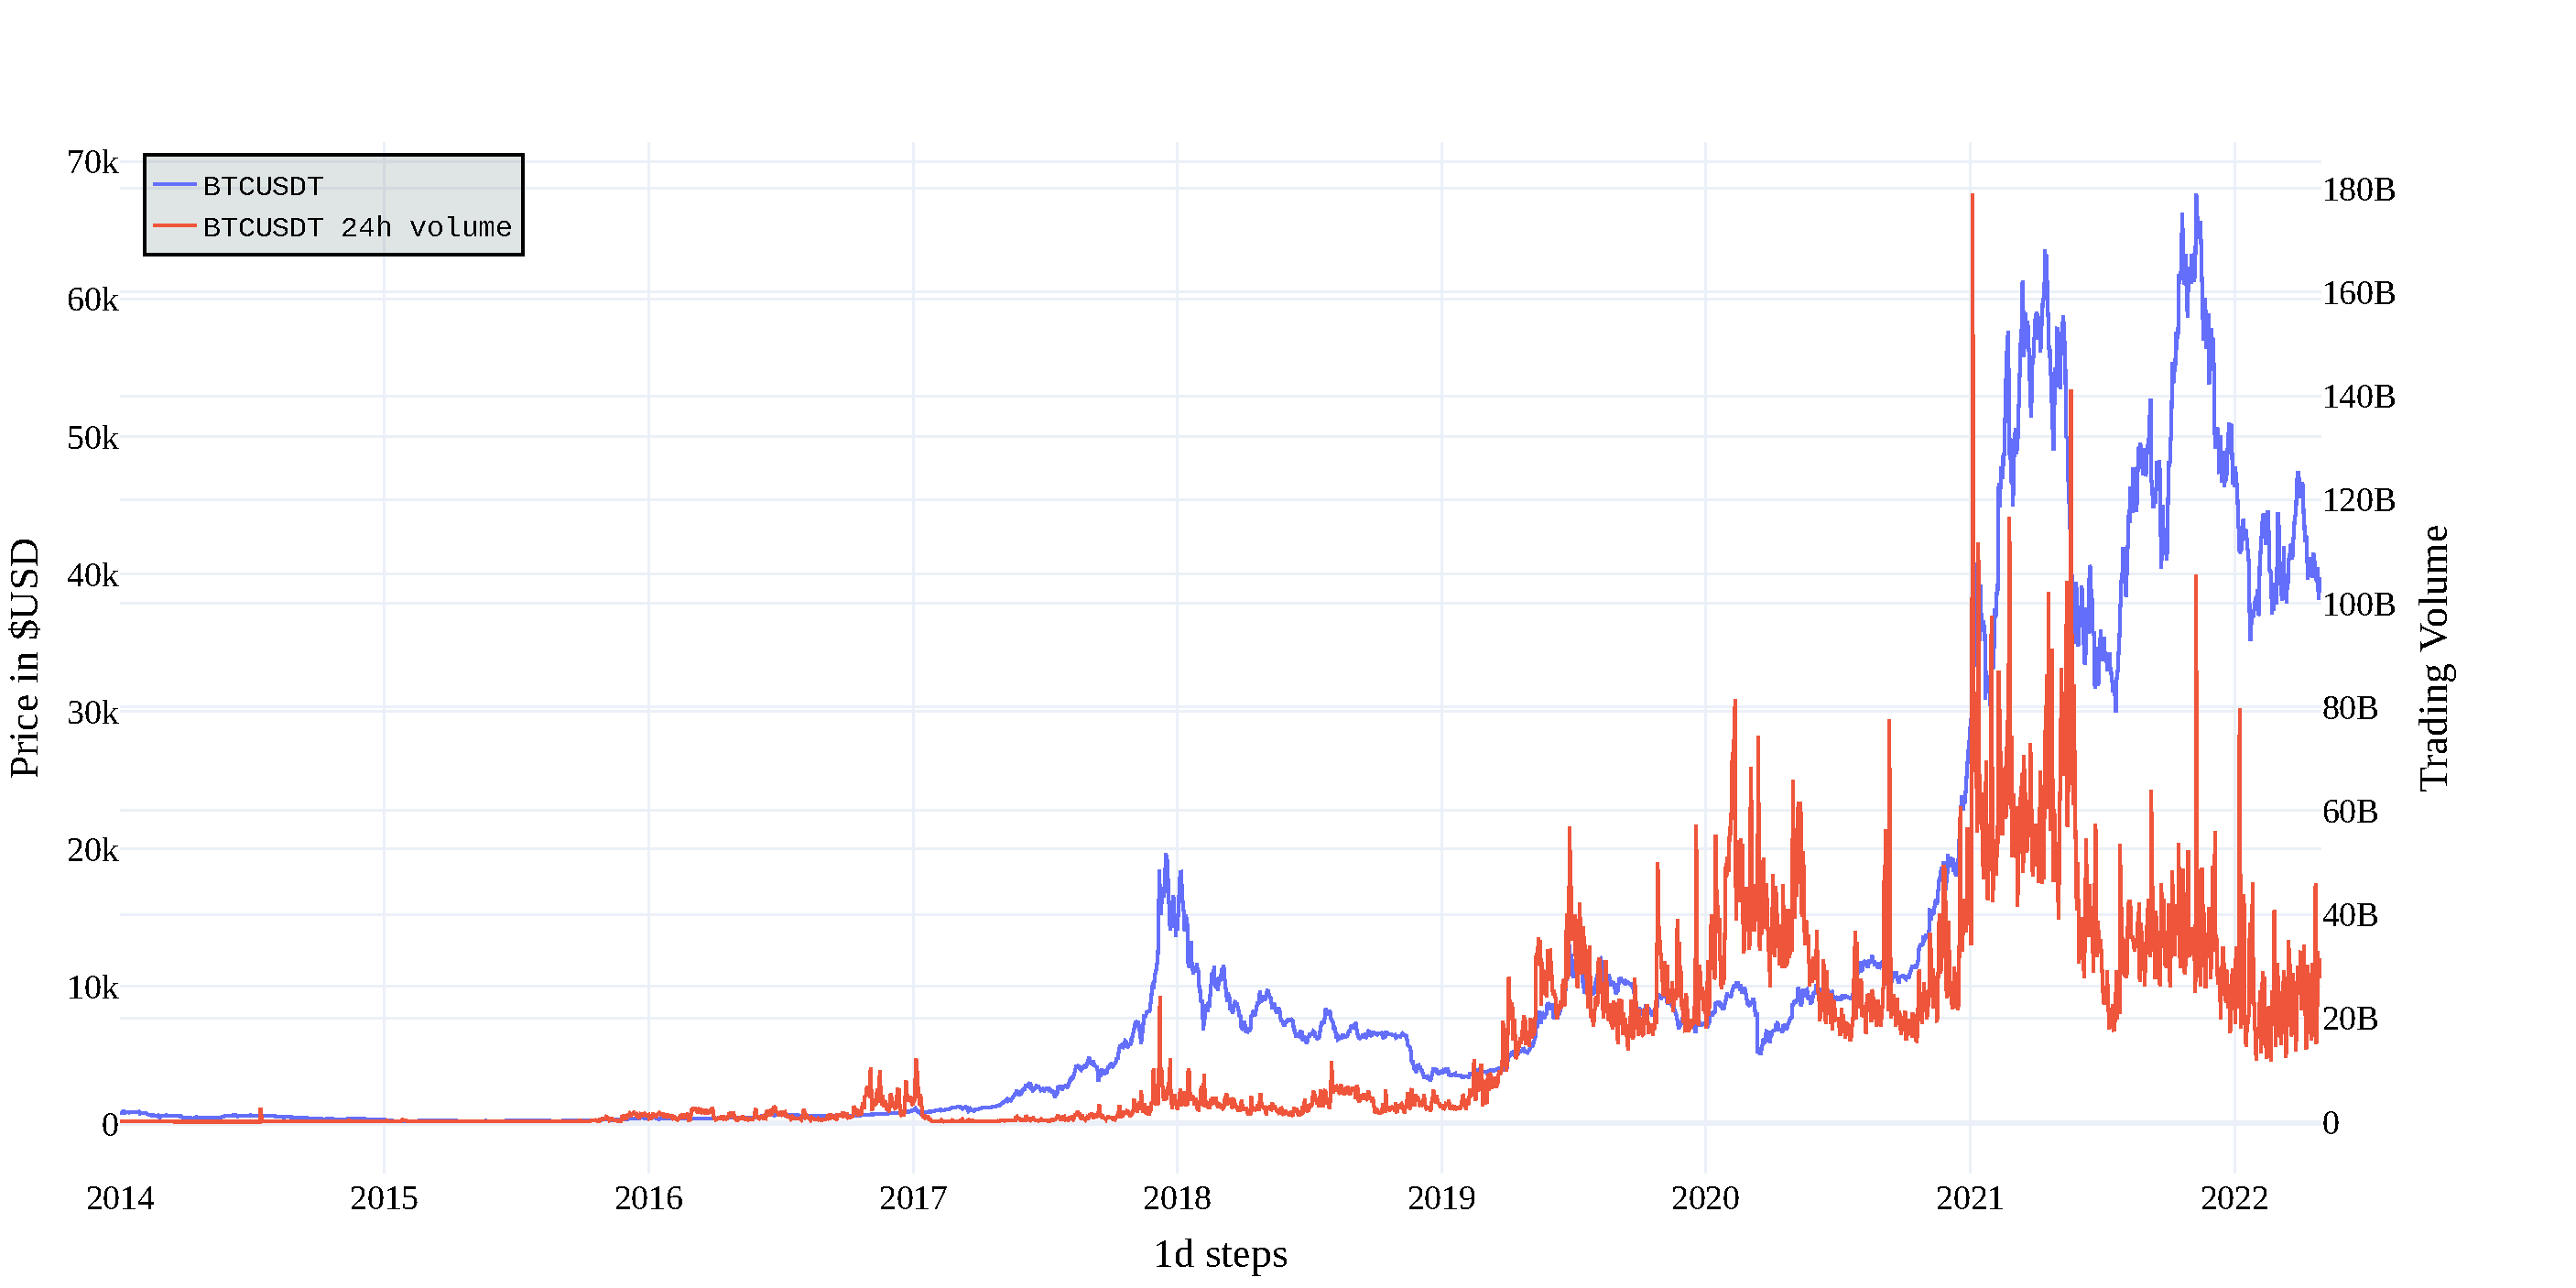
\includegraphics[width=\columnwidth]{figures/24volume-lin.pdf}
    \caption{Linear graph comparison between Bitcoin price and its daily volume traded in \$USD.}
    \label{figure-24volume-lin}
\end{figure}

\begin{figure}[!t]
    \centering
    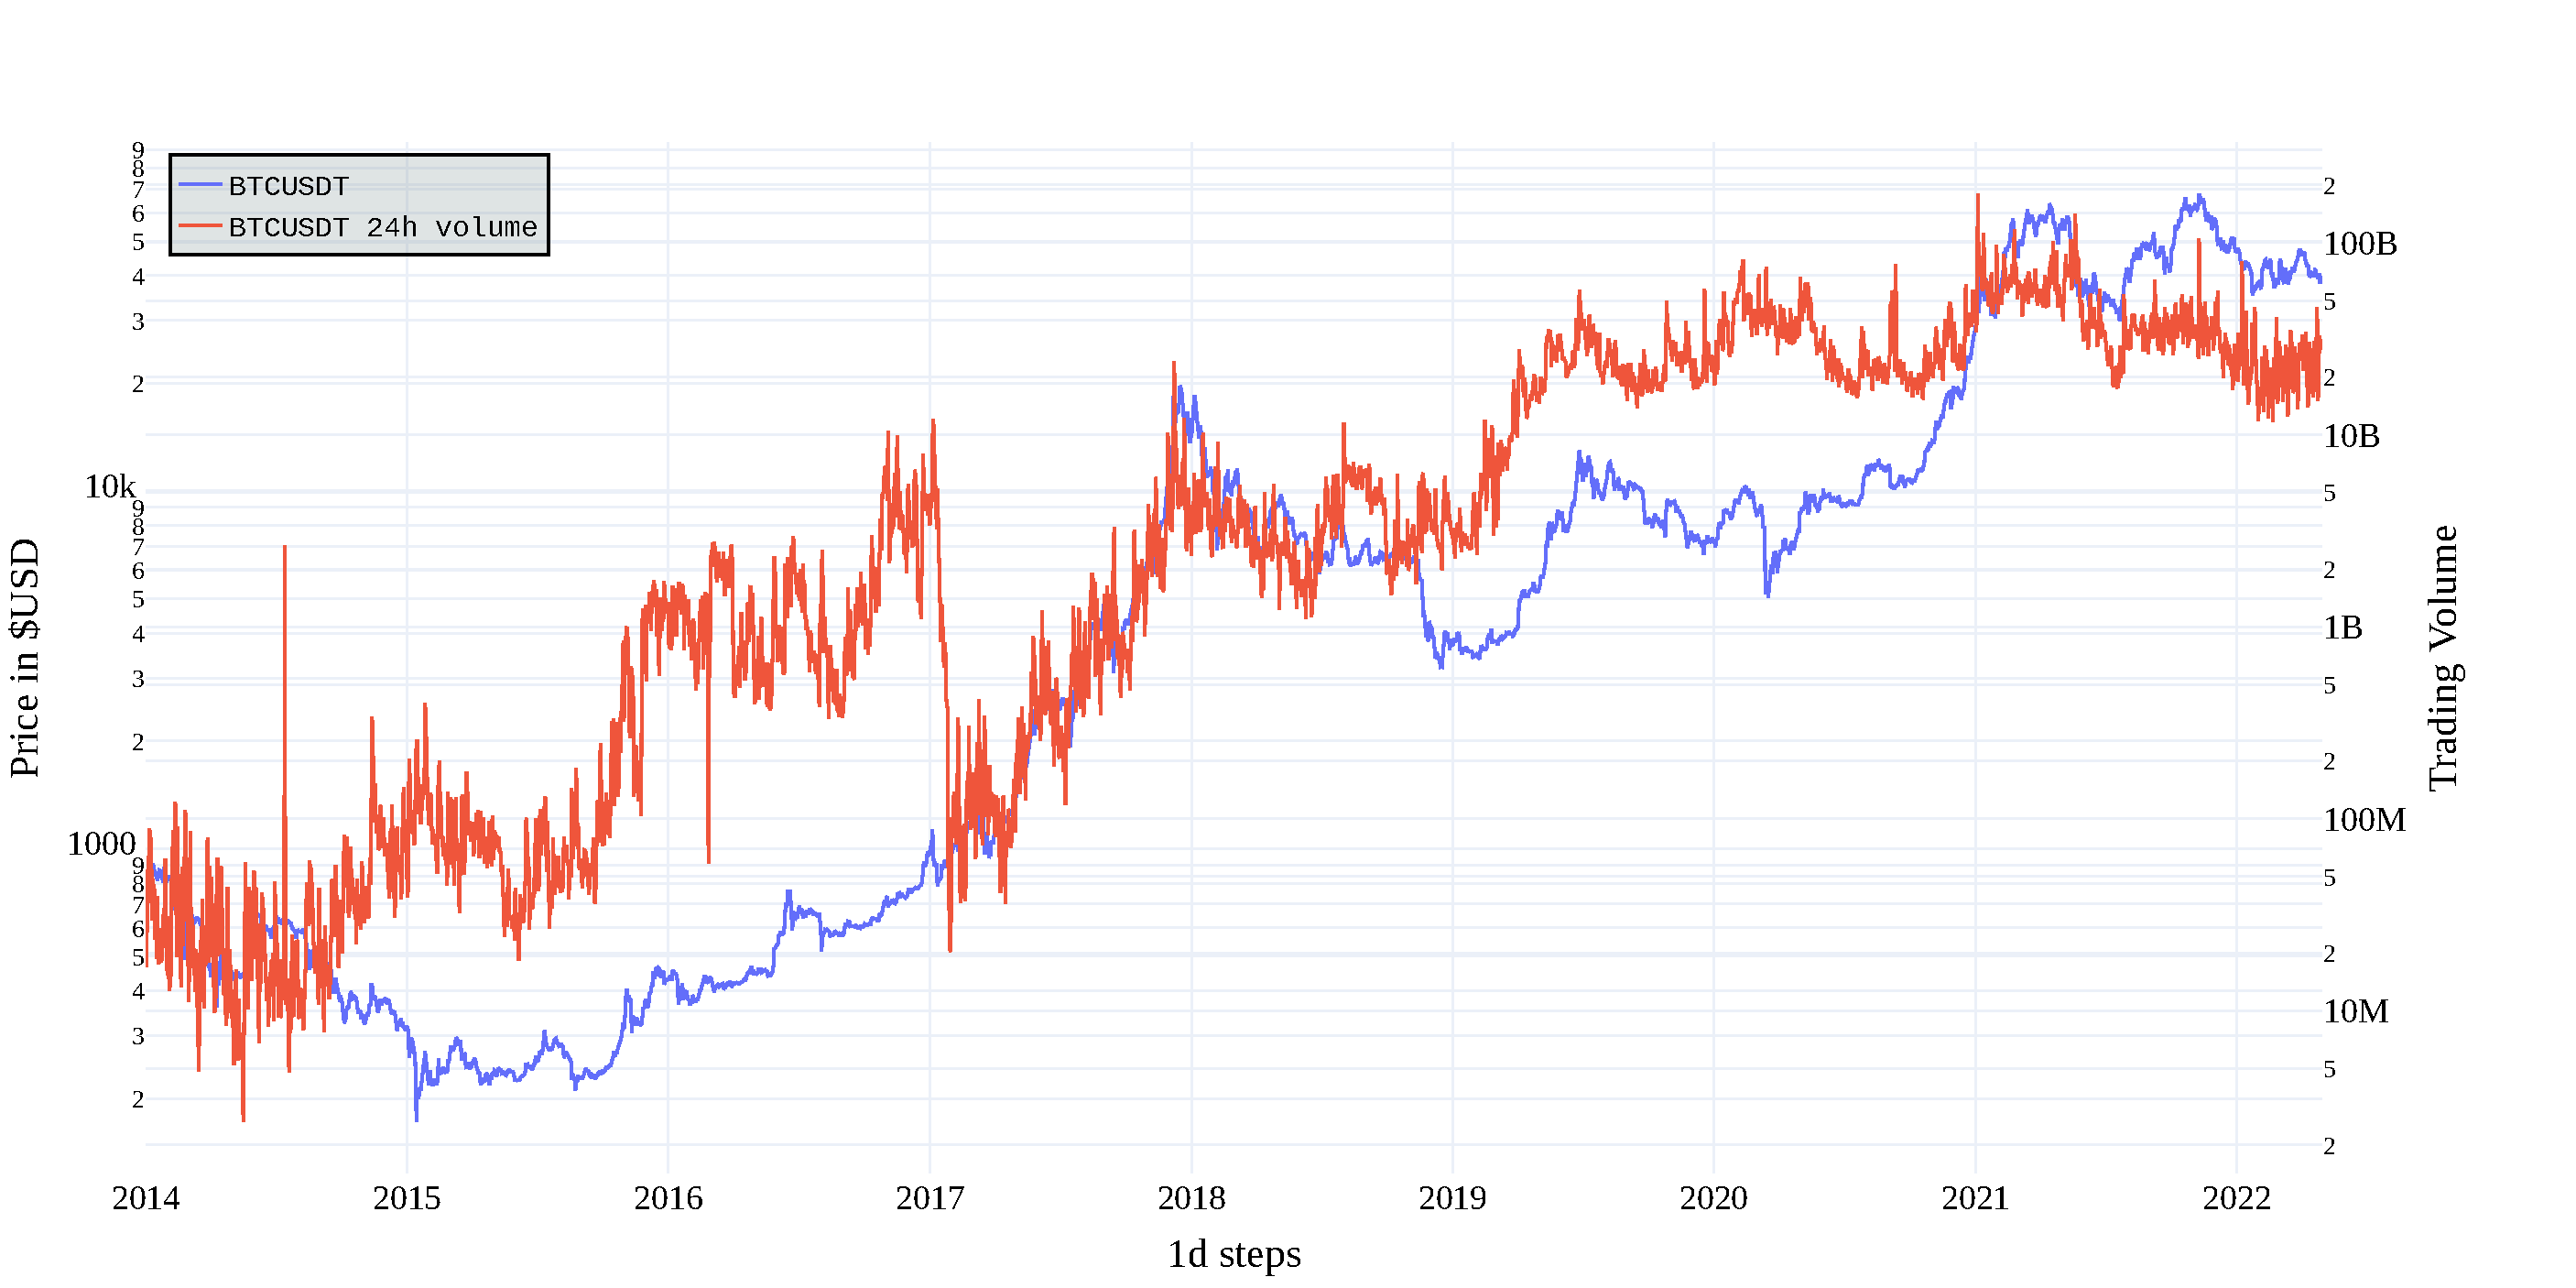
\includegraphics[width=\columnwidth]{figures/24volume-log.pdf}
    \caption{Log-log graph comparing the Bitcoin price and its daily volume traded in \$USD.}
    \label{figure-24volume-log}
\end{figure}

Next step is to incorporate the daily traded volume with the risk metric. There are two ways to go about it. Either, we incorporate the daily trading volume directly into the risk metric, making the risk higher when more volume is traded and vice versa. Or we incorporate the daily trading volume into the evaluation strategy. That means we will decide to buy or sell not just by the risk metric, but the evaluation algorithm will take the daily trading volume into consideration, too.

Choosing the first approach, incorporating the trading volume into the risk metric itself, we can go about it in the following way. First, we compute the smooth rolling average of the last 7 days of the trading volume. We take this average and normalize it between values 0.5 and -0.5. Then we take the original risk metric, and we add some reduced value of the trading volume average on top of it, making the risk higher if more volume has been traded in the last 7 days and lower if less volume has been traded.

The following formula is produced, the $'$ sign represent the normalization between $0$--$1$. The symbols BTC\_SMA represents the Bitcoin smooth moving average and VOL\_SMA represent the trading volume moving average. I~found that the coefficient of $0.2$ works quite well.
$$risk = \left(\frac{\mathit{BTC\_SMA}_{50 days}}{\mathit{BTC\_SMA}_{50 weeks}}\right)' + \left(\mathit{VOL\_SMA}_{7 days}' - 0.5\right) * 0.2$$

When optimizing it for diminishing returns, we just alter the original metric:
$$risk = \left[\frac{\mathit{BTC\_SMA}_{50 days}}{\mathit{BTC\_SMA}_{50 weeks}} * \log_{10}(d)\right]' + \left(\mathit{VOL\_SMA}_{7 days}' - 0.5\right) * 0.2$$

In Figure~\ref{figure-24volume-7sma} the 7 days moving average of trading volume can be seen. In Figure~\ref{figure-24volume-riskmetric} the base metric is benchmarked against the correlated risk metric, dashed line denote the diminishing returns optimizations.

\begin{figure}[!t]
    \centering
    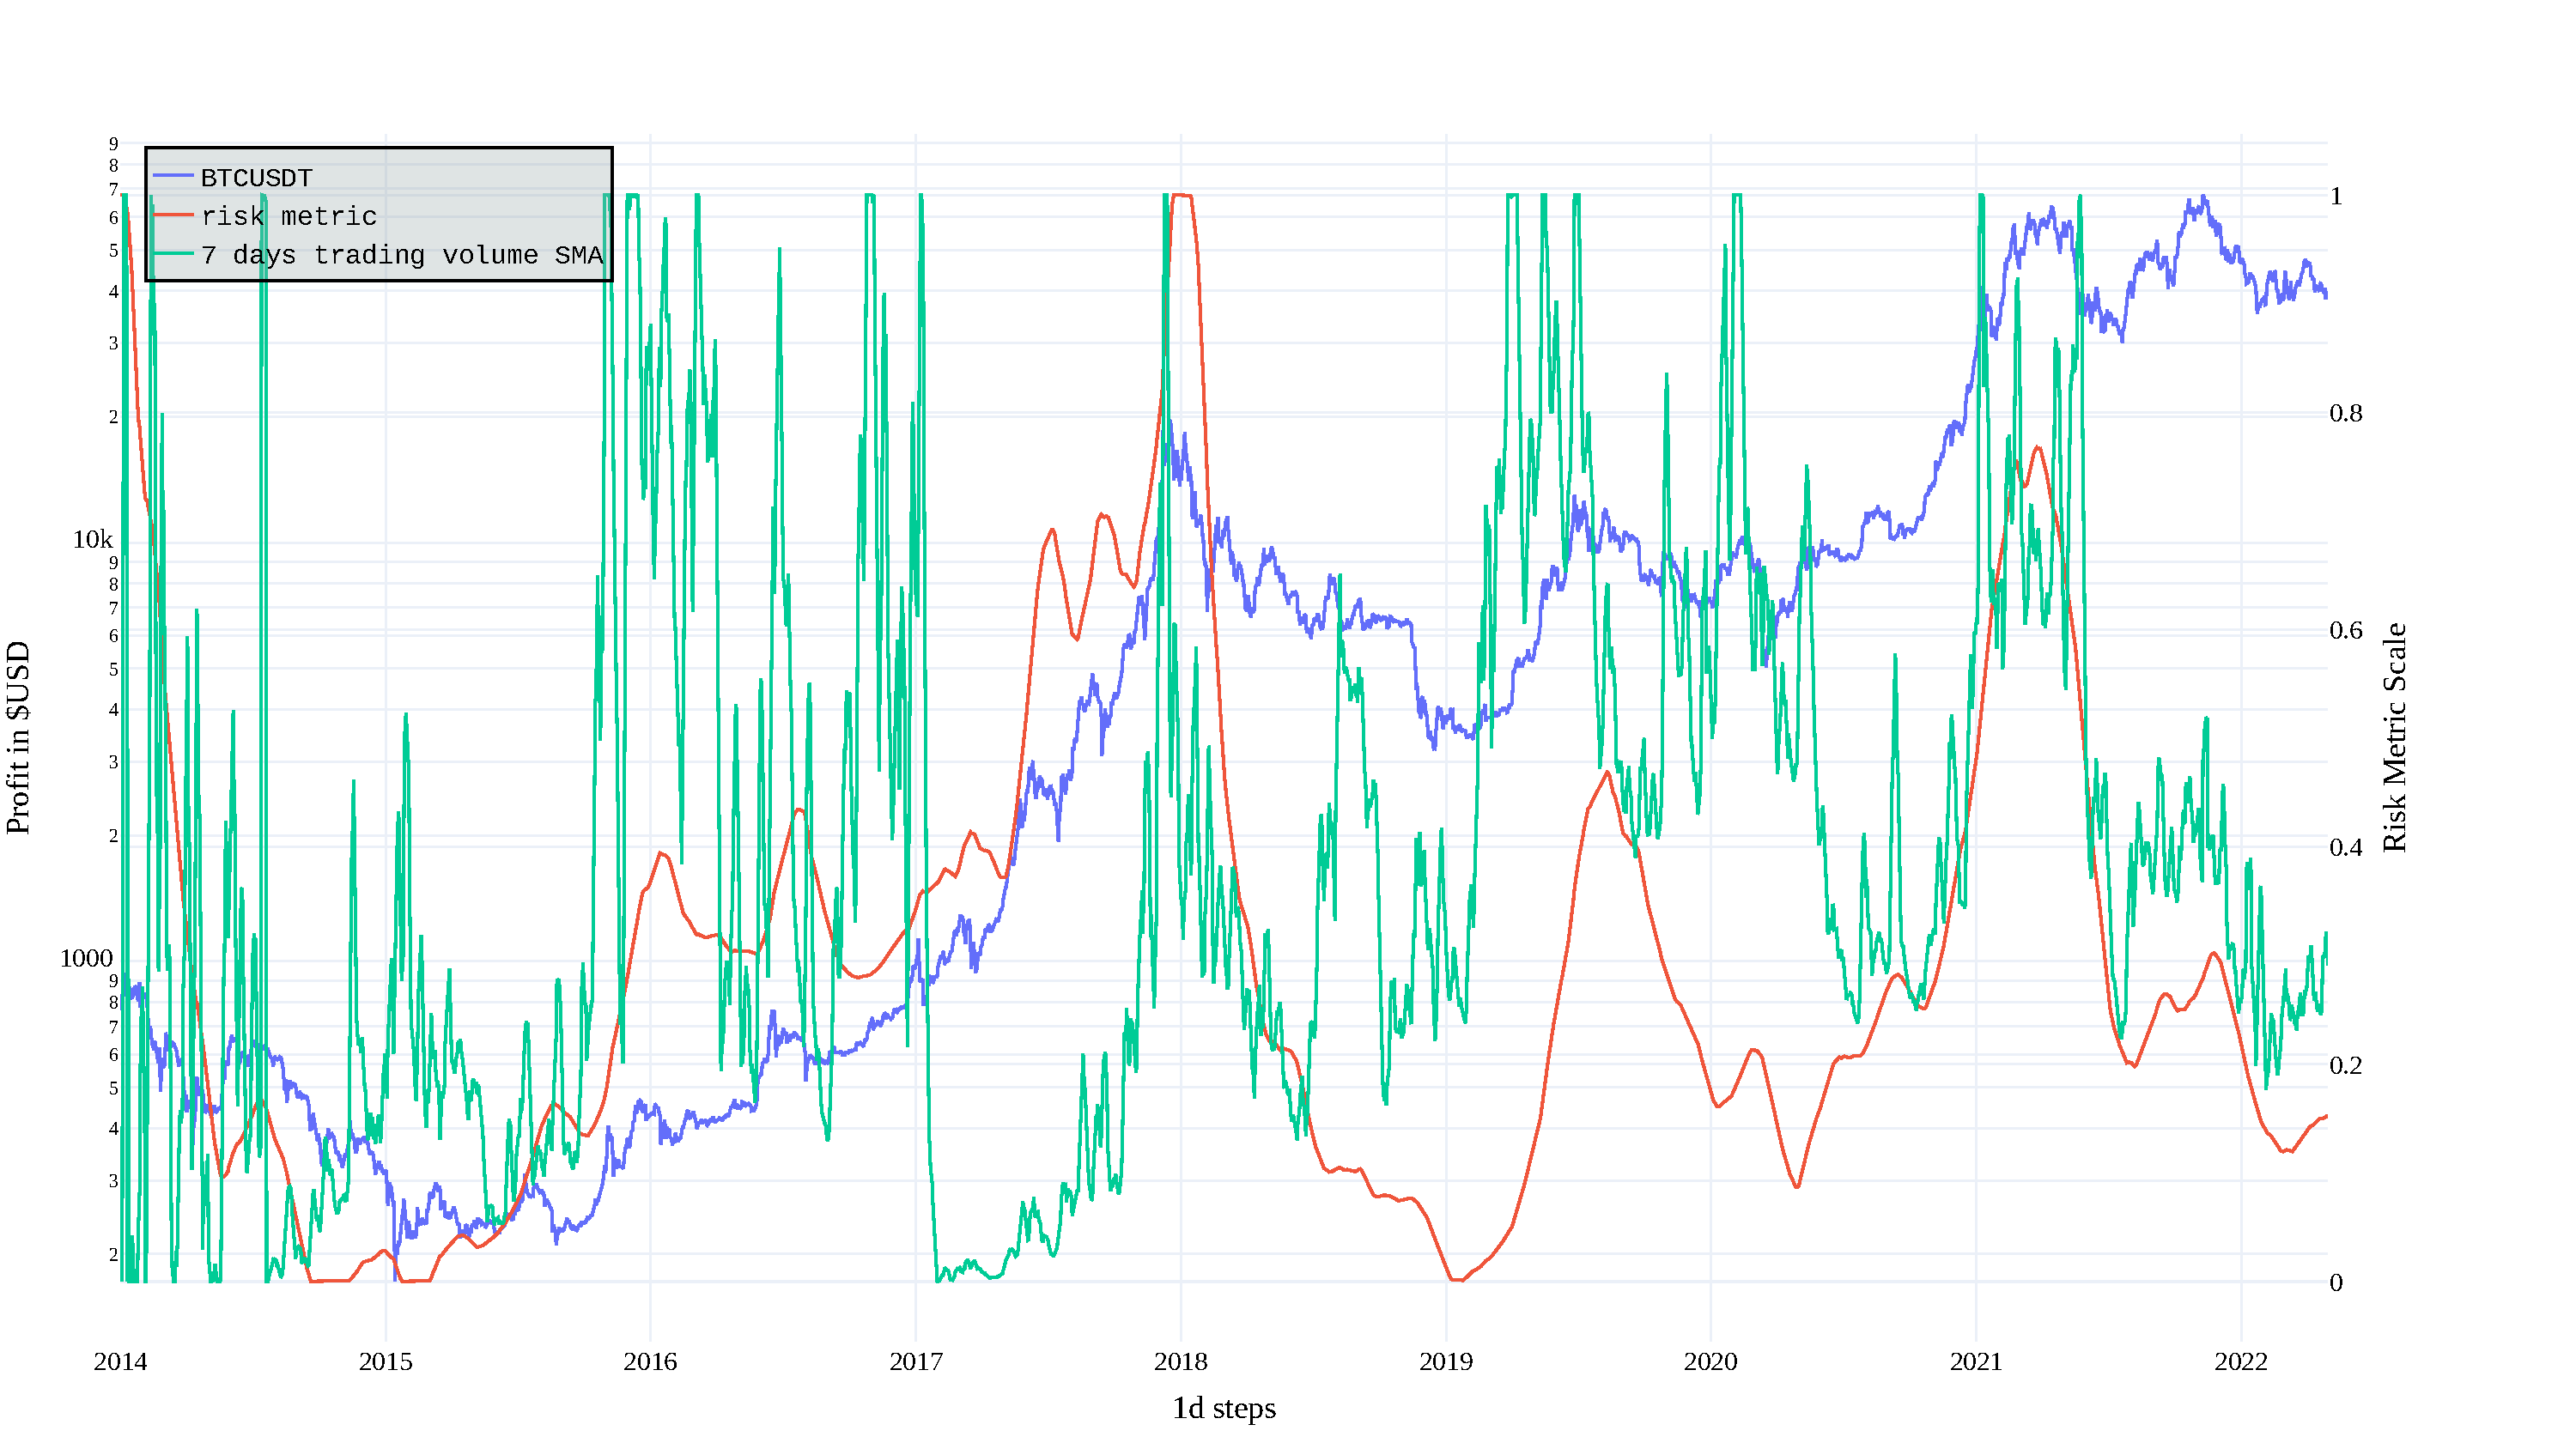
\includegraphics[width=\columnwidth]{figures/24volume-7sma.pdf}
    \caption{Visualization of the 7 days moving average of the daily traded volume on top of the risk metric. The volume was limited between values 0 and 1.}
    \label{figure-24volume-7sma}
\end{figure}

\begin{figure}[!t]
    \centering
    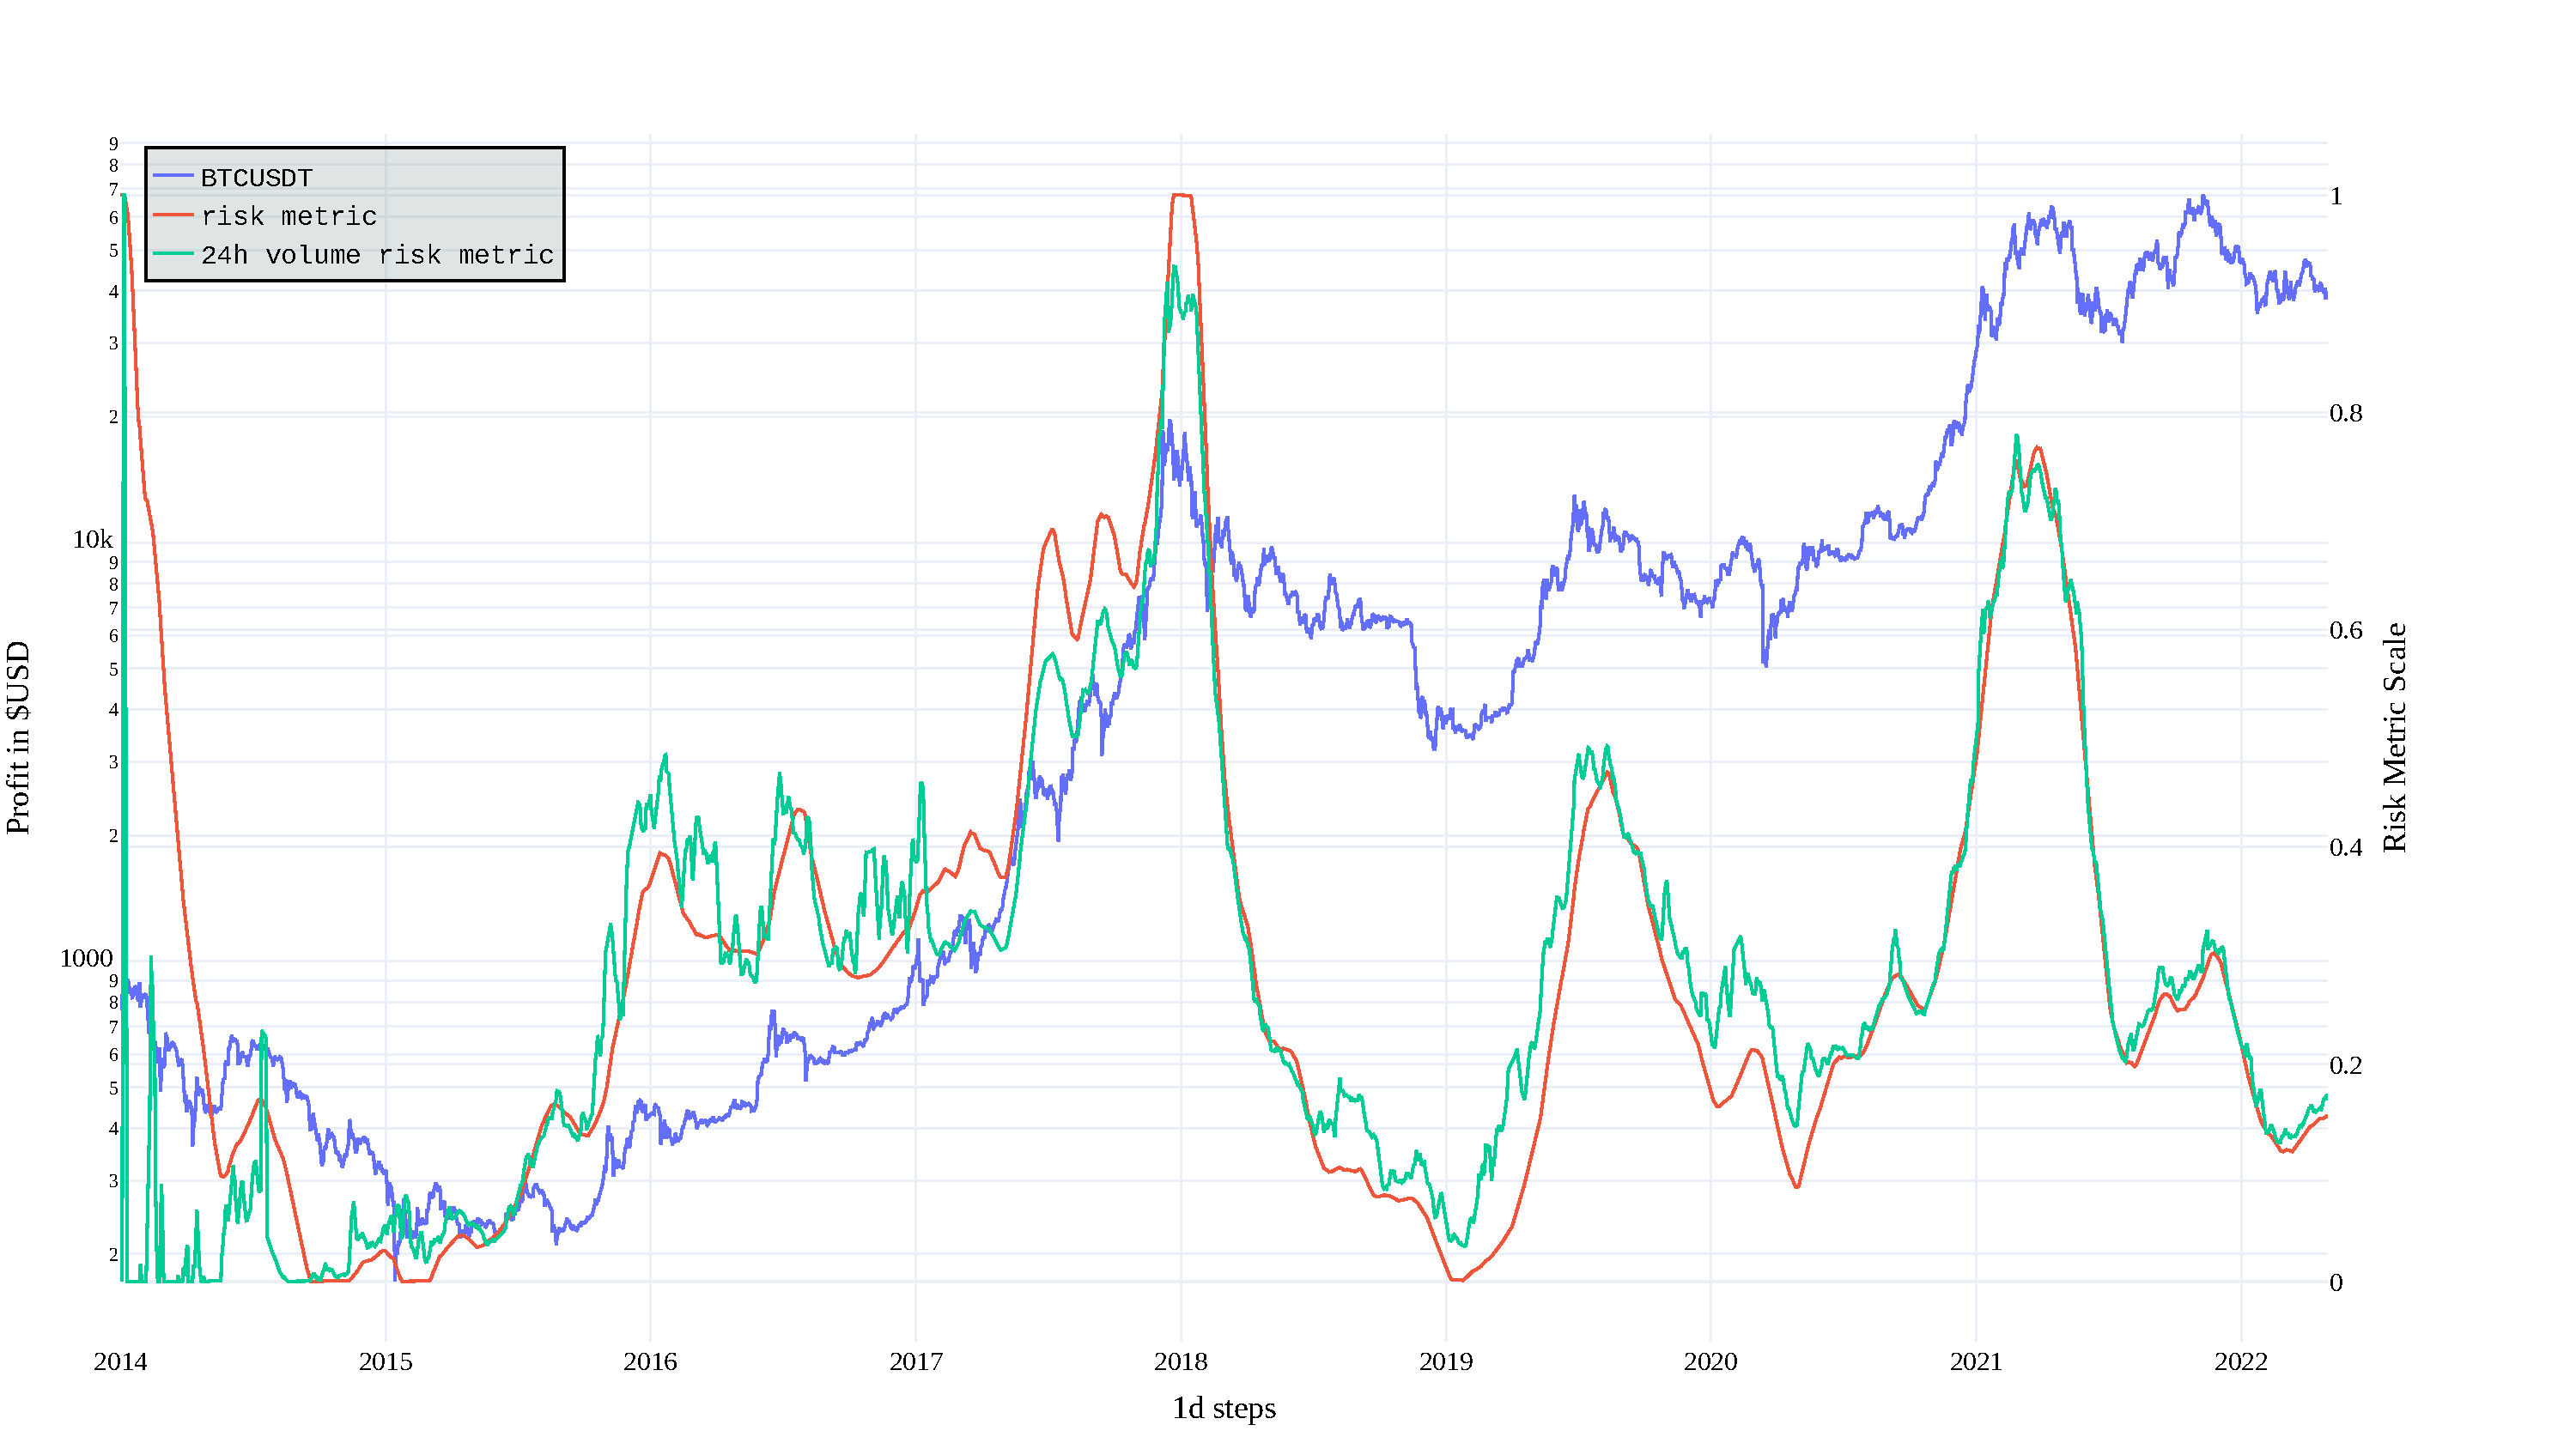
\includegraphics[width=\columnwidth]{figures/24volume-riskmetric.pdf}
    \caption{Logarithmic graph benchmarking the base risk metric against the correlated metric with daily volume.}
    \label{figure-24volume-riskmetric}
\end{figure}


\subsection*{Machine Learning Optimization}
\label{subsection-ml-optimization}

In this Section, the last optimization is touched upon. Machine Learning is a very vast subject. For the thesis's purpose, the time series prediction is our subject. Predictions of these types require a good model to learn upon to work well, otherwise the results are questionable at best. In this Section, the time series prediction is used to predict the price of Bitcoin. This result could be later correlated with the previous achieved findings.

The \texttt{AutoTS} Python library~\cite{autots} is used to make the predictions. One of the ways that the machine learning optimization could be incorporated to the other tactics is the following. Every day it would predict the price for the following X (e.g., 10) days. Depending on how well the prediction is, it would either make the risk bigger or smaller.

The forecasts got are too linear and usually too optimistic to be of any bigger use. Some forecast can be seen in Figure~\ref{figure-autots-prediction}
Since the results got are not reliable, the machine learning optimization is not evaluated. Further investigation of the machine learning algorithm would be needed.

\begin{figure}[!t]
    \centering
    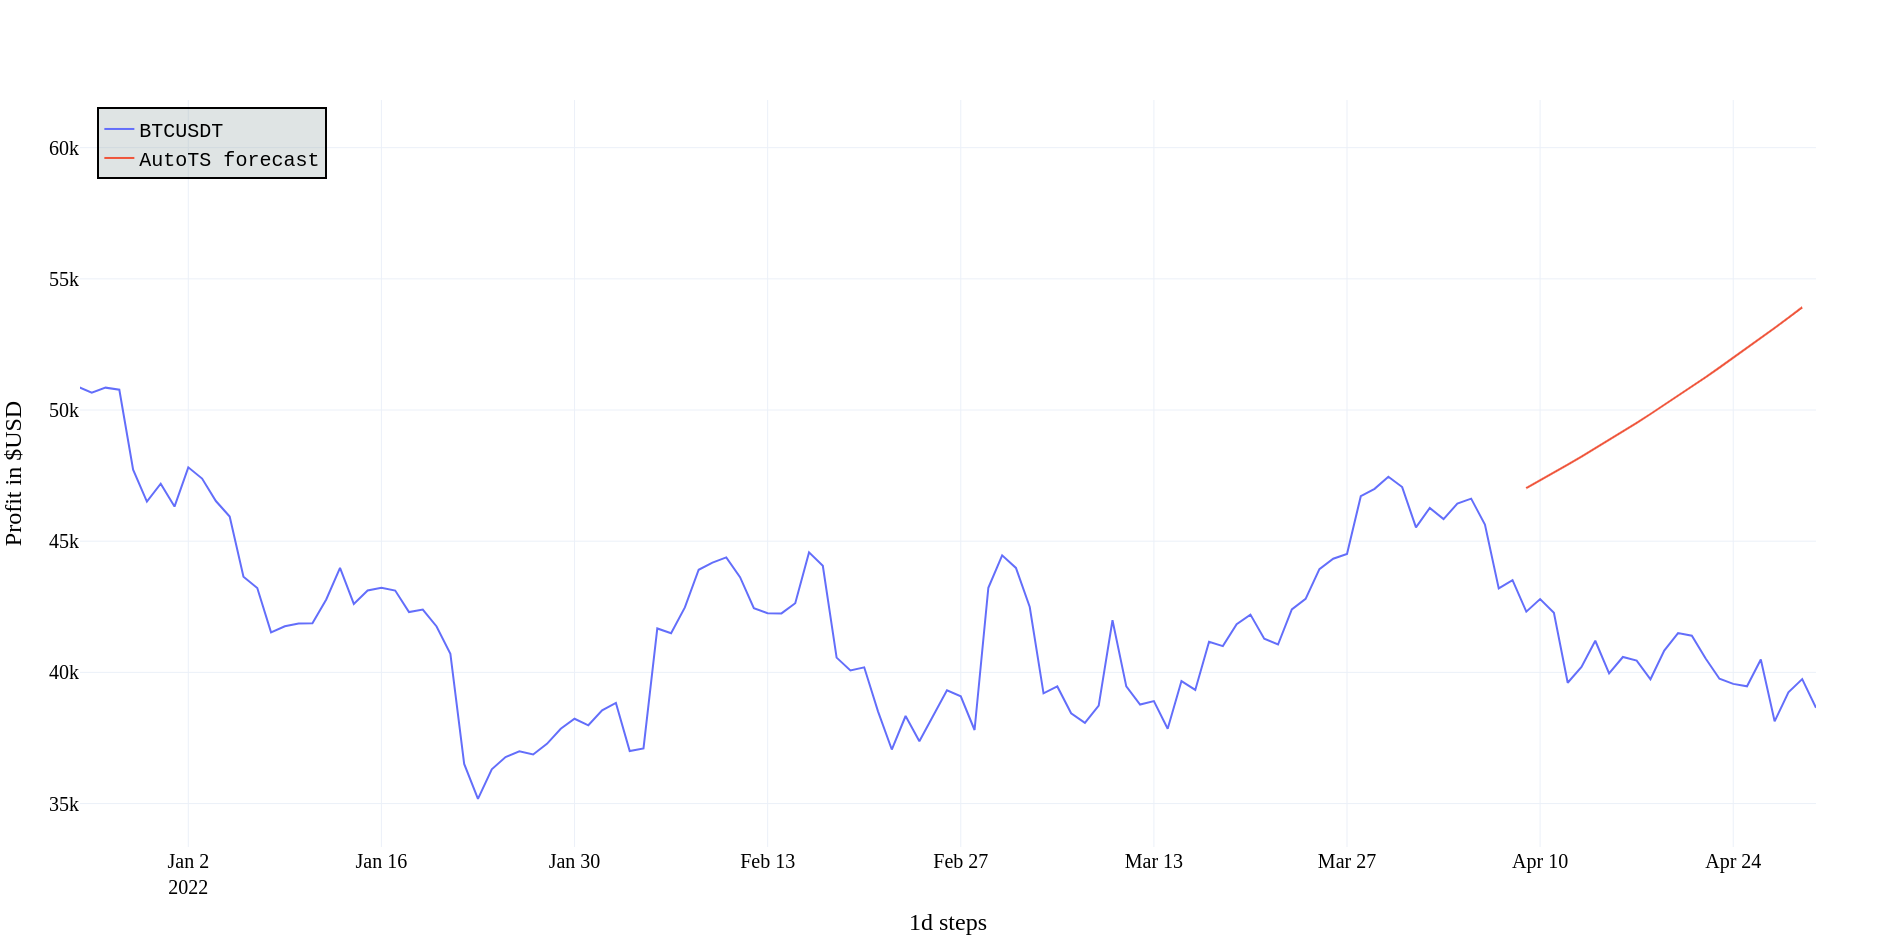
\includegraphics[width=\columnwidth]{figures/autots-prediction.png}
    \caption{AutoTS~\cite{autots} prediction.}
    \label{figure-autots-prediction}
\end{figure}

\section{Evaluating Strategies}
Let us put the implemented strategies to use. In this Section the correct evaluation strategy is found and discussed strategies of Section~\ref{section-strategies} evaluated.

Some of the strategies, like machine learning optimization~\ref{subsection-ml-optimization}, is not evaluated since its usefulness has not been proved in the previous Section.

\subsection*{Finding the Optimal Evaluation Strategy}
One interesting discovery during the testing was that transferring coins to stablecoins when risk gets higher may not be beneficial at all. If the risk keeps on rising, we will lose on the precious gains that come from the rising effect. We will still keep some gains, but not the entirety of it because we transferred a considerable amount of our coins to stablecoins. That is why I~started to consider the fact that we should not only focus on the risk itself, but also on the nature of the direction itself---finding local maxima and minima and minding the slope.

\subsection*{Evaluation Strategy -- Risk Only}
When playing around with the risk values, I~have found good results when using the following values:
\begin{itemize}
    \item $Risk \ge  0.9$: All capital is converted to stablecoins.
    \item $0.8 \le Risk < 0.0$: 60\% converted.
    \item $0.7 \le Risk < 0.8$: 30\% converted.
    \item $0.6 \le Risk < 0.7$: Capital is in coins only.
    \item $0.5 \le Risk < 0.6$: Capital is in coins only.
    \item $0.4 \le Risk < 0.5$: Capital is in coins only.
    \item $0.3 \le Risk < 0.4$: Capital is in coins only.
    \item $0.2 \le Risk < 0.3$: Capital is in coins only.
    \item $0.1 \le Risk < 0.2$: Capital is in coins only.
    \item $Risk < 0.1$: Capital is in coins only.
\end{itemize}

The results can be seen in the joint Figure~\ref{figure-combined-riskmetric} of all the evaluation strategies under the name "RiskMetricStrategyRiskLogic". It did better than HODLing, but only barely, finishing at $\$41,700$ compared to HODL's $\$37,600$.

\subsection*{Evaluation Strategy -- Local Extrema Only}
\label{subsection-local-extrema}
When looking at the extrema, we look at the nature of the risk's direction. When we encounter a local maximum, we transfer all the coins to stablecoins, and when we encounter a minimum, we transfer those stablecoins back to coins---selling high, buying low.

Of course, the extremes itself cannot be determined on the particular day, we never know if the metric is going to go up or down. That is an ideal situation that can never occur. For the calculation, five points from each side are taken into the consideration---this prevents too many extrema next to each other, which would not be useful. Because of this, we can only be certain of the extrema after 5 days have passed since the extreme occurred. As an example, for a local minimum that occurred on 15th January, we would actually put the buy order in on 20th January.

The results are again seen in the joint Figure~\ref{figure-combined-riskmetric} as the "RiskMetricStrategyRealExtrema" line. The strategy did quite well. At the end the investor has around $\$98,400$ compared to the HODL's $\$37,600$. That is approximately 2.6 times higher turn out!

\subsection*{Evaluation Strategy -- Risk And Extrema Combination}
Even though the results of the local extrema look very good, I~cannot wonder if the two indicators cannot be somehow combined. The combination works as follows. When a local maximum is encountered, we sell, and when we encounter a local minimum, we buy. That is the same behavior as previously. The twist is that when we buy, we check the risk metric. If the risk is high, we only buy so much and when it is low, we sell less.

I~have prepared 3 combined strategies, the first checks the risk both when selling and buying, the second focuses on optimizing selling only, and the third on the buy only. Results can again be seen in the aforementioned Figure~\ref{figure-combined-riskmetric}.

The first combined strategy performed the worst out of the three. The second one is the average, and the third performed the best, still not outperforming the local extrema strategy, ending at around $\$90,660$. We must keep in mind, that even though the third strategy was the best out of the three, that does not mean that optimizing for buy only is a profitable strategy, it just means that it is less damaging to the portfolio profit. That being said, all of the combined strategies outperformed the risk-only strategy.

\begin{figure}[!t]
    \centering
    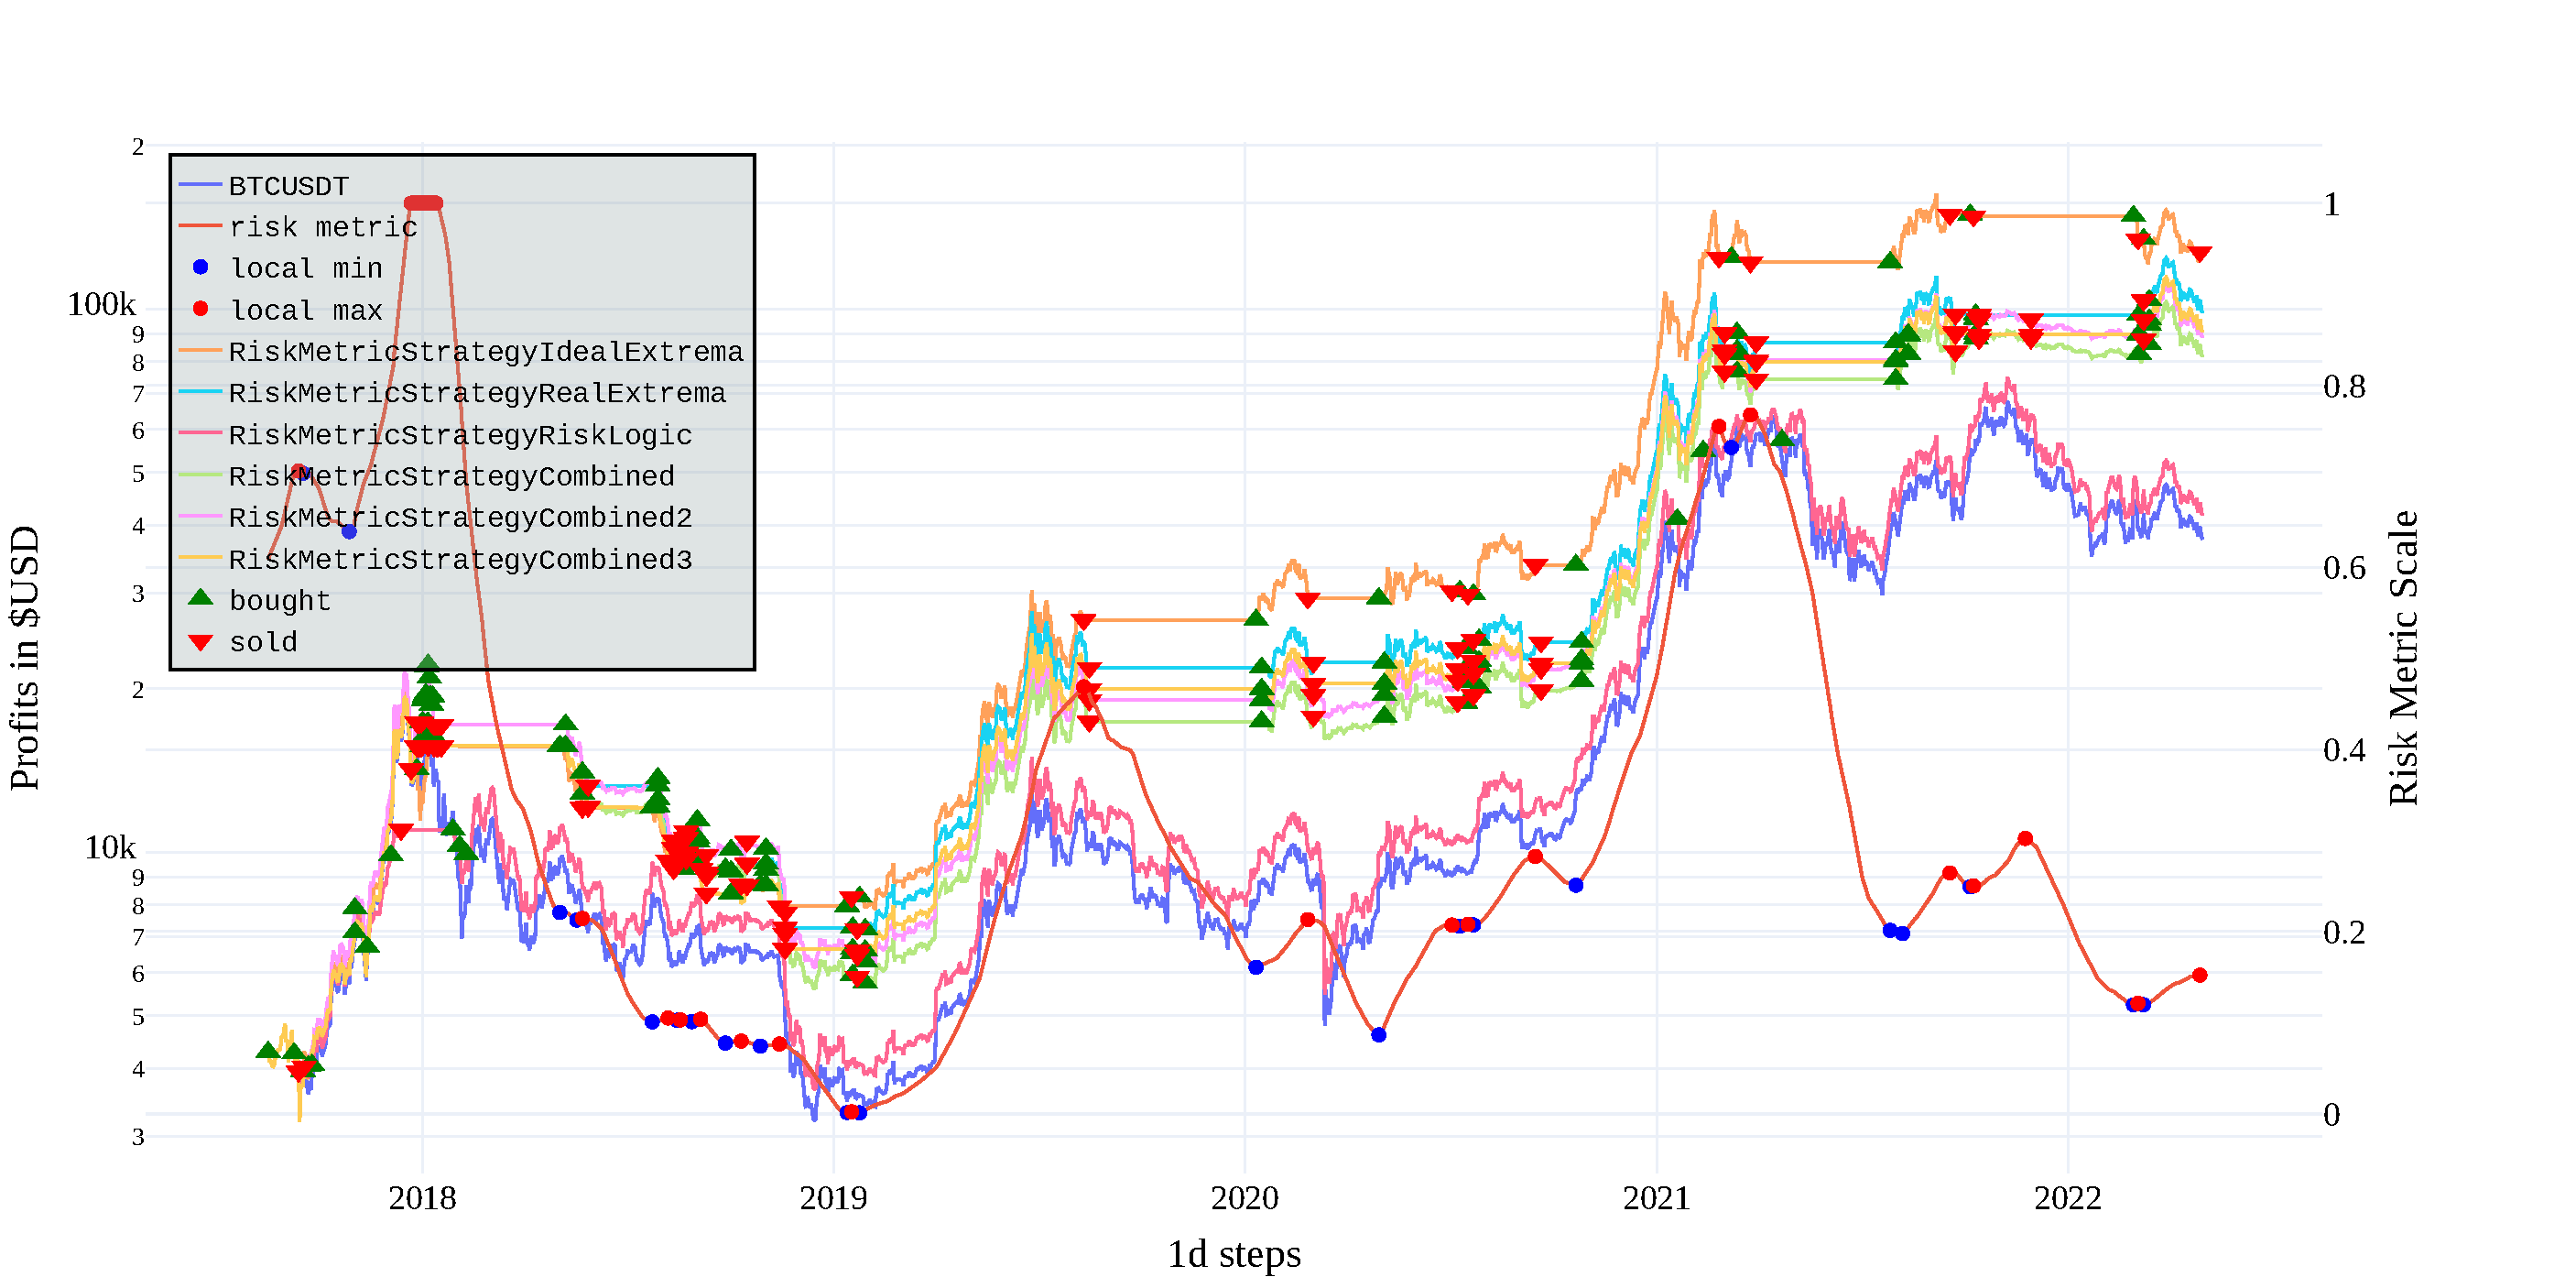
\includegraphics[width=\columnwidth]{figures/combined-riskmetric.pdf}
    \caption{Showcase of evaluation strategies for the same risk metric.}
    \label{figure-combined-riskmetric}
\end{figure}

\subsection*{Evaluation Strategy -- DCA}
\label{subsection-eval-dca}
We have traded the coins to stablecoins and back, when we simulated the strategies so far. The other option is to never sell the coins we have, but rather buy additional coins when the opportunity presents itself. That is the point of the DCA (dollar cost averaging) strategy, explained in detail in Section~\ref{section-dca}.

Depending on the risk's value, we will change our DCA investments accordingly. When the risk is high, less money or no money is invested, and when the risk is low, we try to invest the most money we have. To benchmark this strategy in a reasonable fashion, there will be no portfolio limit to what we can invest. To benchmark against regular DCA, we will take the overall \$USD invested and invest it over regular DCA, which invests the same amount of money each day. The real life scenario, where a portfolio could use the variable strategy, would be a portfolio that is dynamic and can offer to take money from other assets. Alternatively, a person that invests once in a while may look at the current risk and adjust his investment accordingly.

I~tried a few different evaluation strategies during the simulations. The one I~used at first is defined as follows:
\begin{itemize}
    \item $Risk \ge  0.7$: Do not invest.
    \item $0.6 \le Risk < 0.7$: Invest sum x1.
    \item $0.5 \le Risk < 0.6$: Invest sum x2.
    \item $0.4 \le Risk < 0.5$: Invest sum x3.
    \item $0.3 \le Risk < 0.4$: Invest sum x4.
    \item $0.2 \le Risk < 0.3$: Invest sum x5.
    \item $0.1 \le Risk < 0.2$: Invest sum x6.
    \item $Risk < 0.1$: Invest sum x7.
\end{itemize}

The results were better than the classic DCA strategy, by about 20\%. The strategies are benchmarked by the ratio of profit in \$USD to the total \$USD invested. Higher the ratio, better the strategy.

Next, an evaluation strategy that follows the Fibonacci sequence was tested. It has been proven that the Fibonacci sequence can work really well when working with financial markets~\cite{investopedia:fibonacci}, so I~gave it a try. The strategy is defined as follows:
\begin{itemize}
    \item $Risk \ge  0.9$: Do not invest.
    \item $0.8 \le Risk < 0.9$: Invest sum x1.
    \item $0.7 \le Risk < 0.8$: Invest sum x1.
    \item $0.6 \le Risk < 0.7$: Invest sum x2.
    \item $0.5 \le Risk < 0.6$: Invest sum x3.
    \item $0.4 \le Risk < 0.5$: Invest sum x5.
    \item $0.3 \le Risk < 0.4$: Invest sum x8.
    \item $0.2 \le Risk < 0.3$: Invest sum x13.
    \item $0.1 \le Risk < 0.2$: Invest sum x21.
    \item $Risk < 0.1$: Invest sum x34.
\end{itemize}

As you can see, the sequence is in a perfect mathematical order. And the results are positive, being around 13\% better than the previous strategy, and about 36\% better than the classic DCA. That is a solid improvement. It is interesting that Fibonacci can work well in an unexpected way.

I~tried to optimize the sequence once more, restricting the investment only under the 0.7 risk and removing the second number 1 of the sequence. The strategy acts as follows:
\begin{itemize}
    \item $Risk \ge  0.7$: Do not invest.
    \item $0.6 \le Risk < 0.7$: Invest sum x1.
    \item $0.5 \le Risk < 0.6$: Invest sum x2.
    \item $0.4 \le Risk < 0.5$: Invest sum x3.
    \item $0.3 \le Risk < 0.4$: Invest sum x5.
    \item $0.2 \le Risk < 0.3$: Invest sum x8.
    \item $0.1 \le Risk < 0.2$: Invest sum x13.
    \item $Risk < 0.1$: Invest sum x21.
\end{itemize}

This strategy is better to the general investing, since a multiple of 21 is less demanding than a multiple of 34. The strategy performed better, but only by a hair. It is 0.4\% percent better than the previous optimizations. A~really minor improvement.

All results can be seen in the joint Figure~\ref{figure-dca-investing}, the primary axis y scale follows the profitable ratio. You can see that the two last strategies overlap almost completely. An interesting observation is that the DCA strategies only get better overtime. That makes, since they need time to make advantage of the fluctuations in the market, and that cannot happen immediately.

The final ratio of profit against the amount invested are as follows:
\begin{itemize}
    \item Classic DCA: 40.2
    \item Risk optimized DCA: 48.15
    \item Risk-Fibonacci DCA: 54.72
    \item Risk-Fibonacci Adjusted DCA: 54.94
\end{itemize}

The numbers represent the return of investment. When looking at the classic DCA value, it tells investors that if they rigorously used the strategy every day from the year 2017 until May 2022, the money invested would have multiplied 40 times. That is a very significant return of investment. Even better for the optimized versions that take the risk into account. One thing must be kept in mind, the trades are done without any exchange feeds. Since the trades are very frequent, profits would be cut to some extent. This could again ve mitigated by using longer interval.

I~tried simulating the strategies with different time intervals for the DCA buy, but similar results were achieved, that is why there is no additional Figure displaying it.

\begin{figure}[!t]
    \centering
    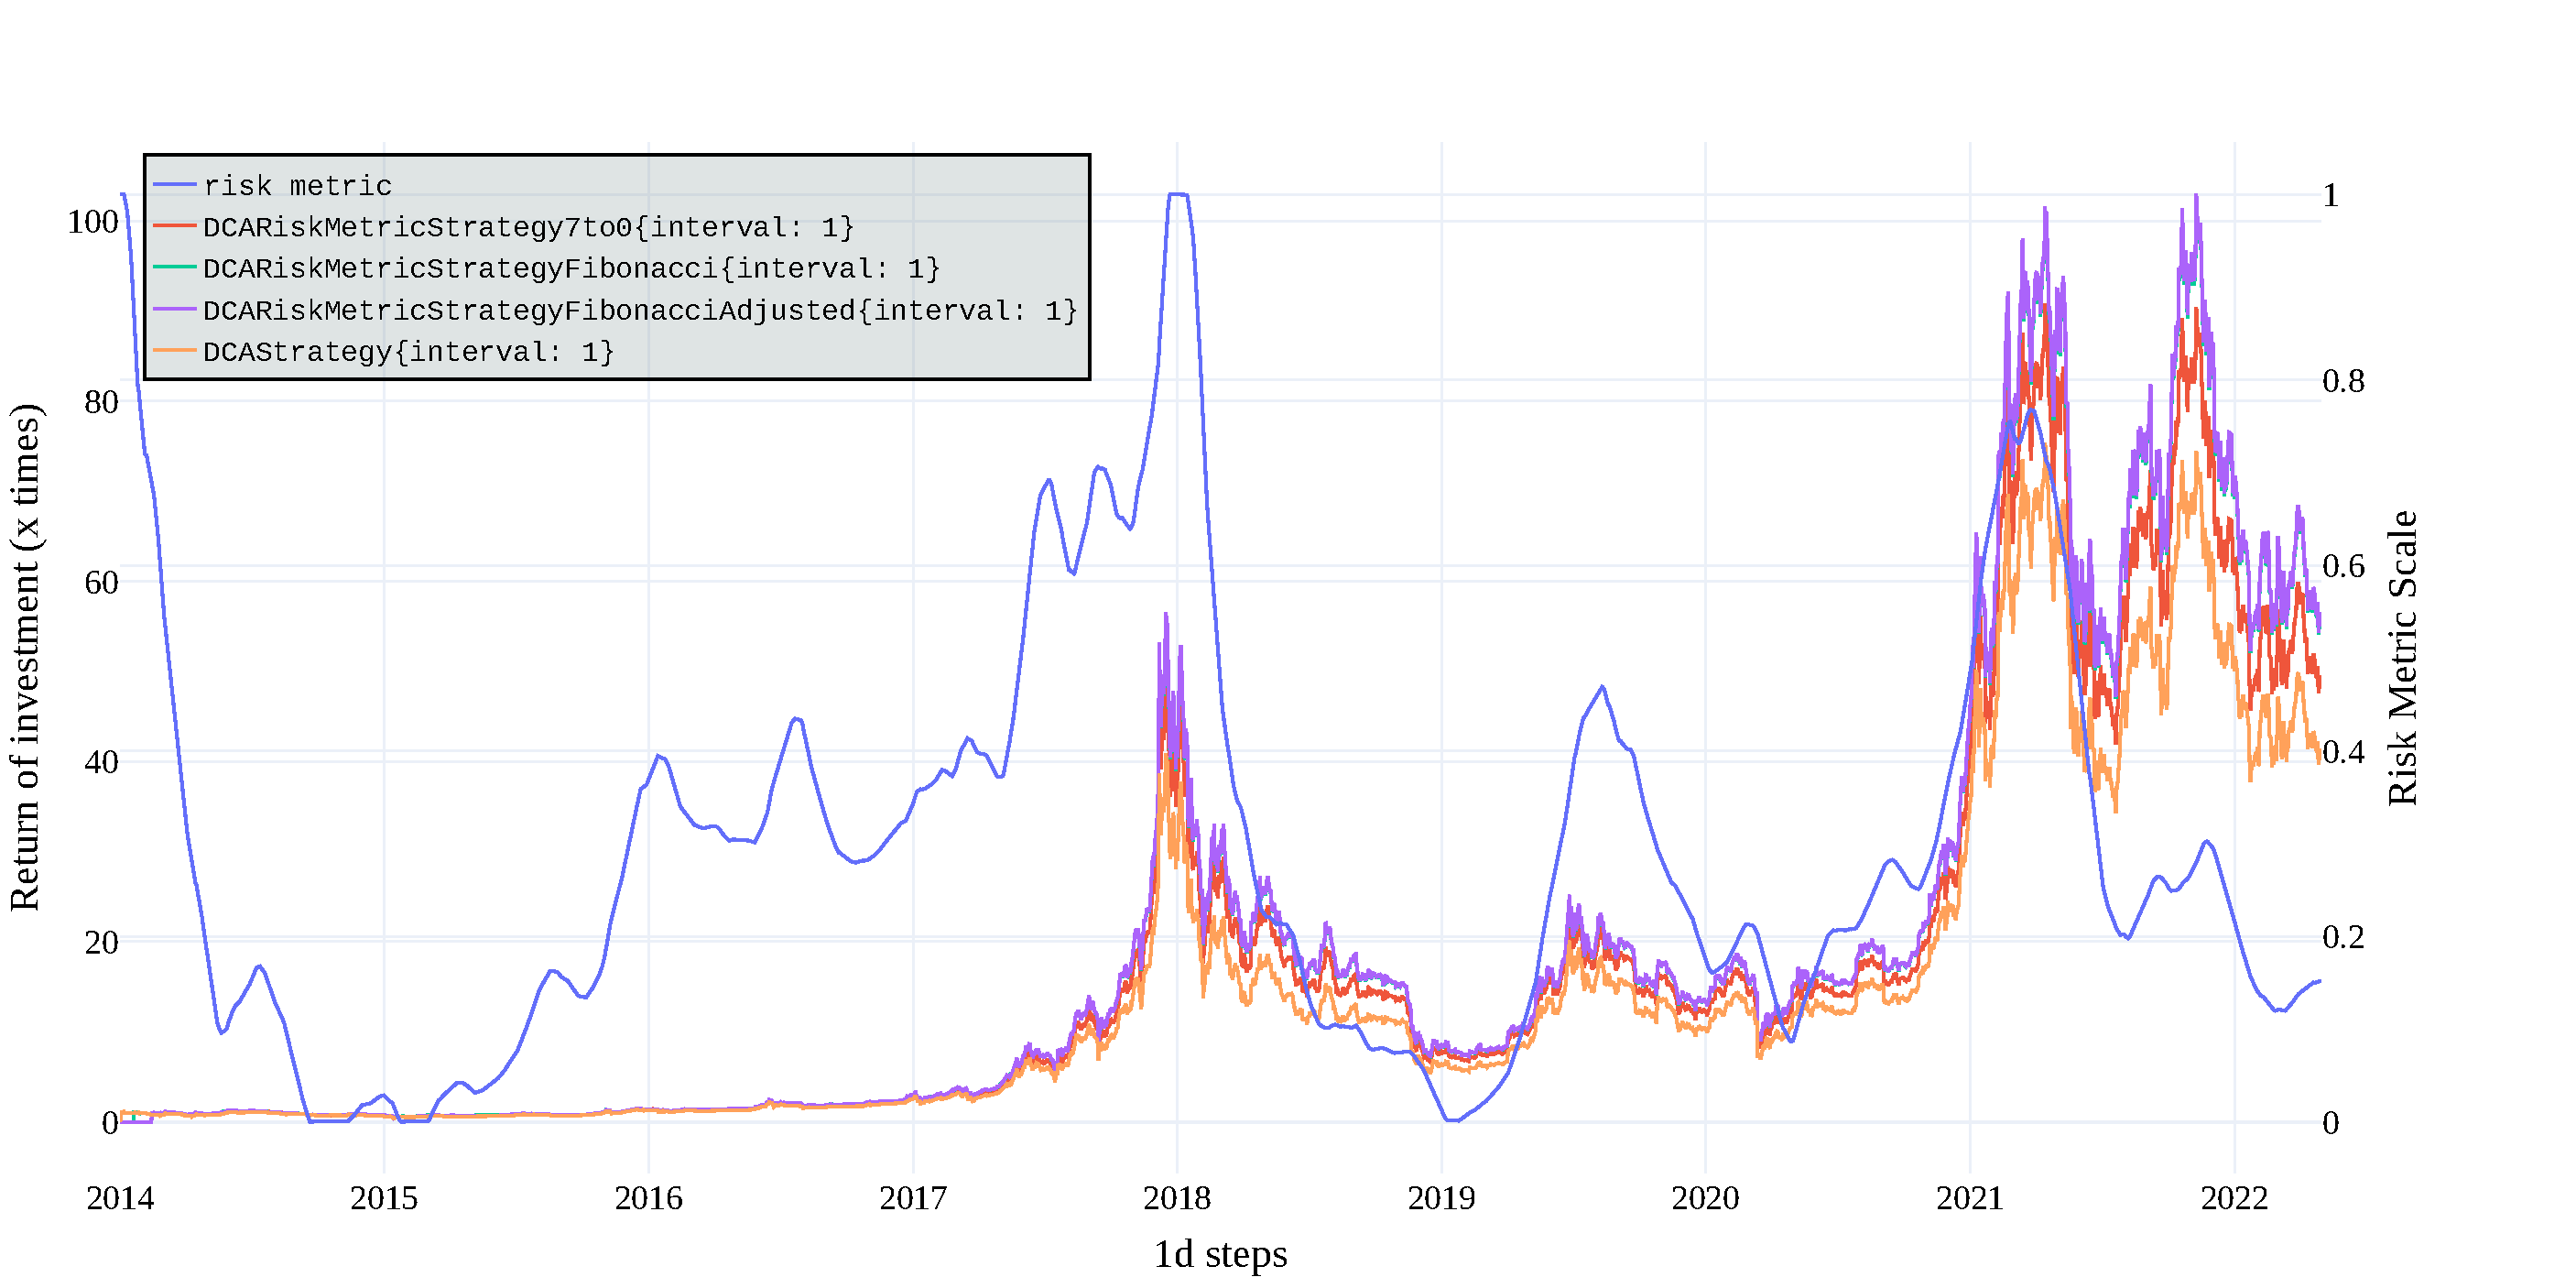
\includegraphics[width=\columnwidth]{figures/combined-dca-investing.pdf}
    \caption{Showcase of evaluation strategies for the DCA strategy.}
    \label{figure-dca-investing}
\end{figure}

\section{Simulating The Risk Metric Optimizations}
\label{section-sim-optimizations}
So far we have defined the possible strategies for calculating risk and found the optimal evaluation strategies. But we only used the default risk metric defined in Section~\ref{subsection-50week50days} without any optimizations. In this Section, optimizations are simulated with the evaluation strategies. Local extrema are chosen for coin to stablecoin transfer, and the adjusted Fibonacci sequence strategy is chosen for the DCA investing.

\subsection*{Local Extrema Evaluation Strategy}
Used evaluation strategy was defined in Section~\ref{subsection-local-extrema}. I~used Bitcoin data beginning from the year 2014 and 2017 for comparison, to see if the newer data experience different phenomena. The results can be seen in Figures~\ref{figure-optimization-longer} and~\ref{figure-optimization-shorter} respectively.

\begin{figure}[!t]
    \centering
    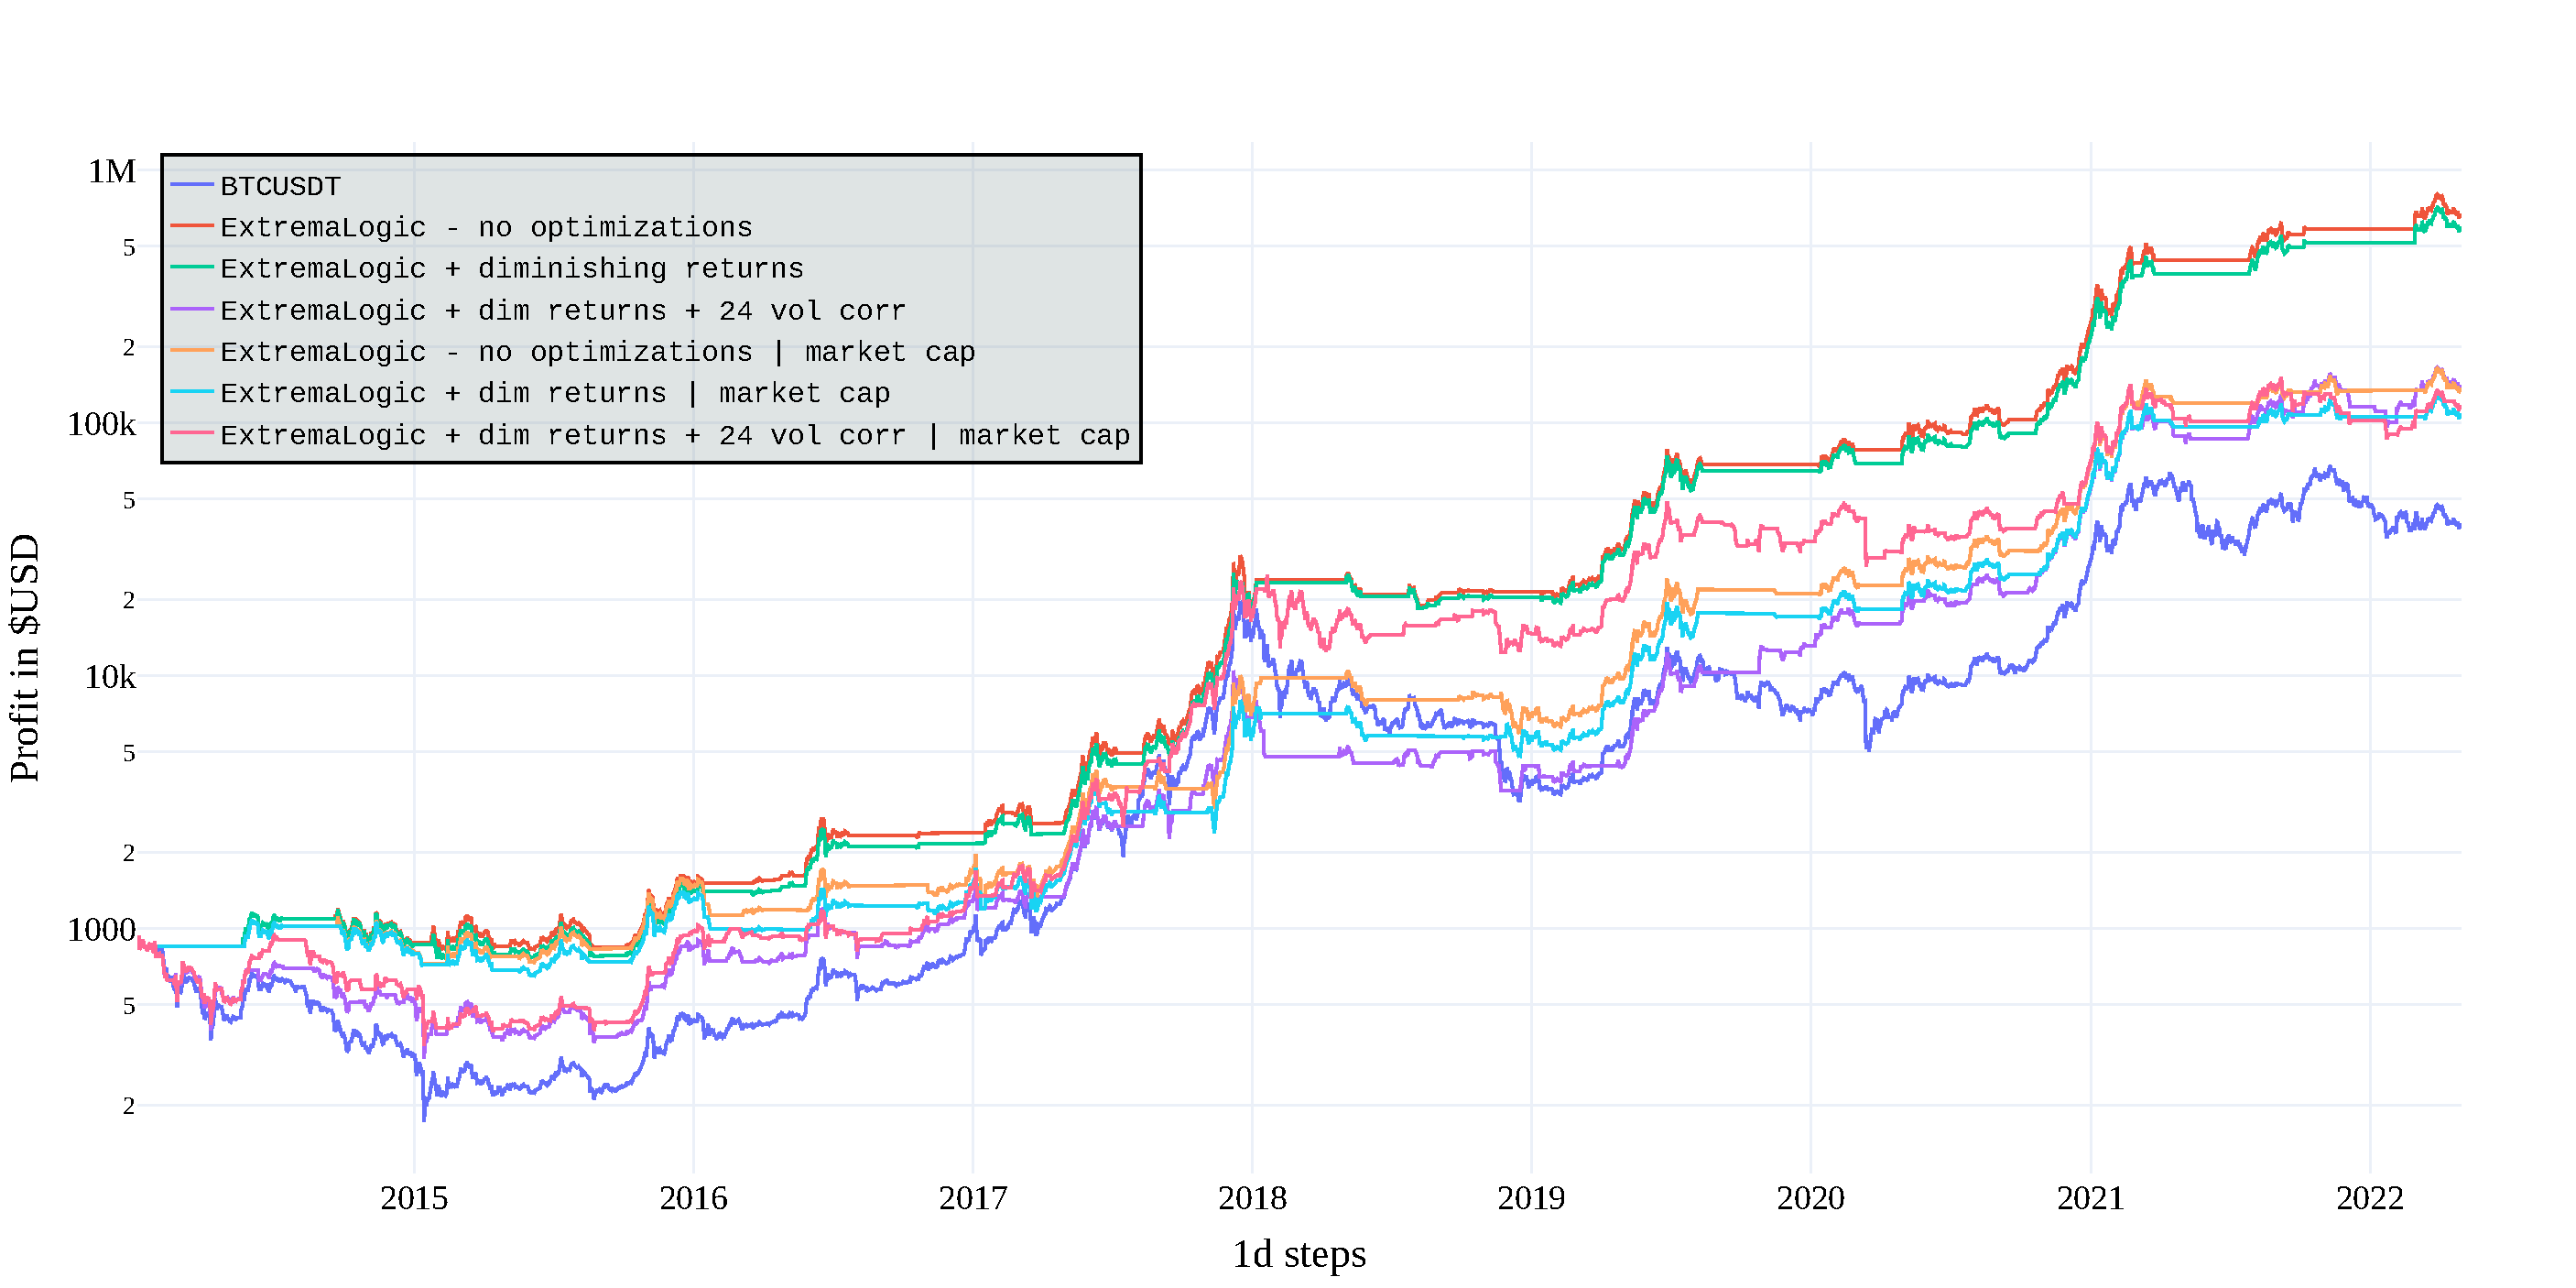
\includegraphics[width=\columnwidth]{figures/evaluation-optimization-longer.pdf}
    \caption{Comparison of risk optimizations used with the local extrema evaluation strategy, dates: Jan 2014--May 2022.}
    \label{figure-optimization-longer}
\end{figure}

\begin{figure}[!t]
    \centering
    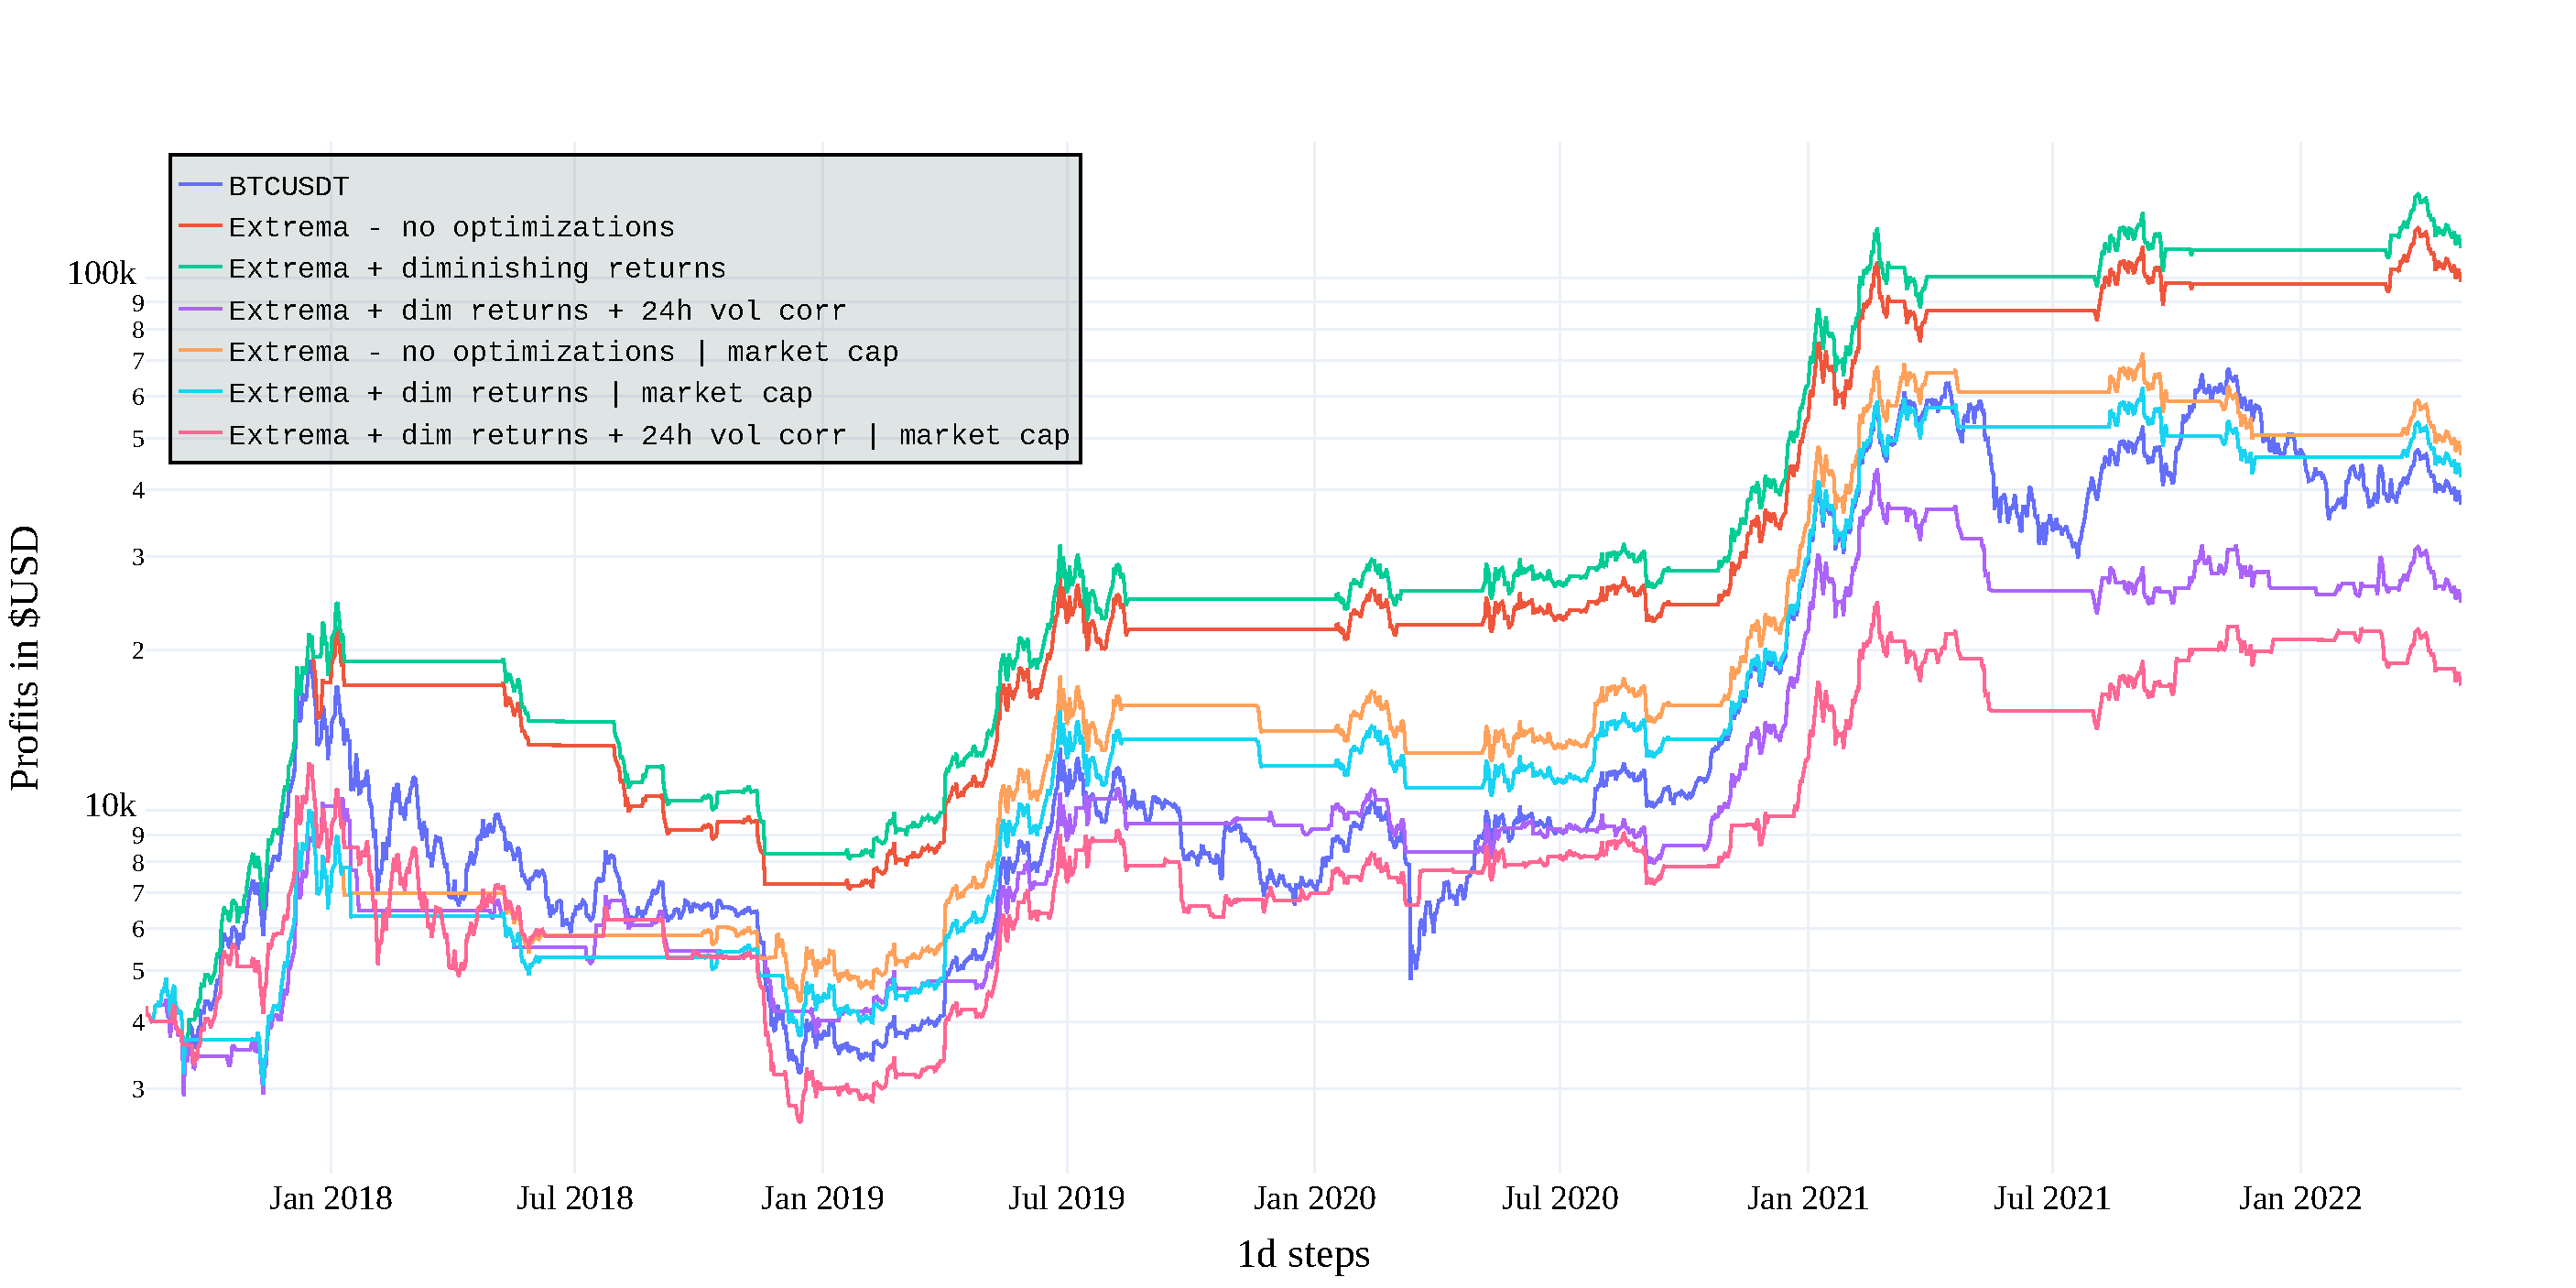
\includegraphics[width=\columnwidth]{figures/evaluation-optimization-shorter.pdf}
    \caption{Comparison of risk optimizations used with the local extrema evaluation strategy. Dates: July 2017--May 2022.}
    \label{figure-optimization-shorter}
\end{figure}

It can be seen that the using the historical Bitcoin data is much preferable to the total market capitalization data. This was to be expected, since the coin in being simulated is Bitcoin itself. Regarding the individual optimizations, using no optimizations and using diminishing returns constantly compete for the first place of best profit. Since diminishing returns prevailed with the newer data, it could mean that this optimization may be more profitable as time goes on. The correlation with the daily volume really underperforms here, taking big loss at the peak of January 2018.

The result is clear. Use the diminishing returns when working with the local extrema evaluation strategy. Bitcoin data should be used for the calculation if working with Bitcoin only. In the results starting in year 2017, the diminishing returns optimizations achieved a result of almost \$114,00 compared previous \$98,400. For comparison with the previous DCA return of investment mentioned in Section~\ref{subsection-eval-dca}, the return of investment of the best strategy ranging from the year 2014 is a multiple of 68.6, starting at \$849.14 in 2014 and ending with the profit of \$58,280 in 2022.

\subsection*{Adjusted Fibonacci Sequence DCA Strategy}
Adjusted Fibonacci sequence strategy was defined in Section~\ref{subsection-eval-dca}. Once again, the Bitcoin data used are of dual character, ranging from the year 2014 and 2017. The results can be seen in Figures~\ref{figure-dca-optimization-longer} and~\ref{figure-dca-optimization-shorter}.

\begin{figure}[!t]
    \centering
    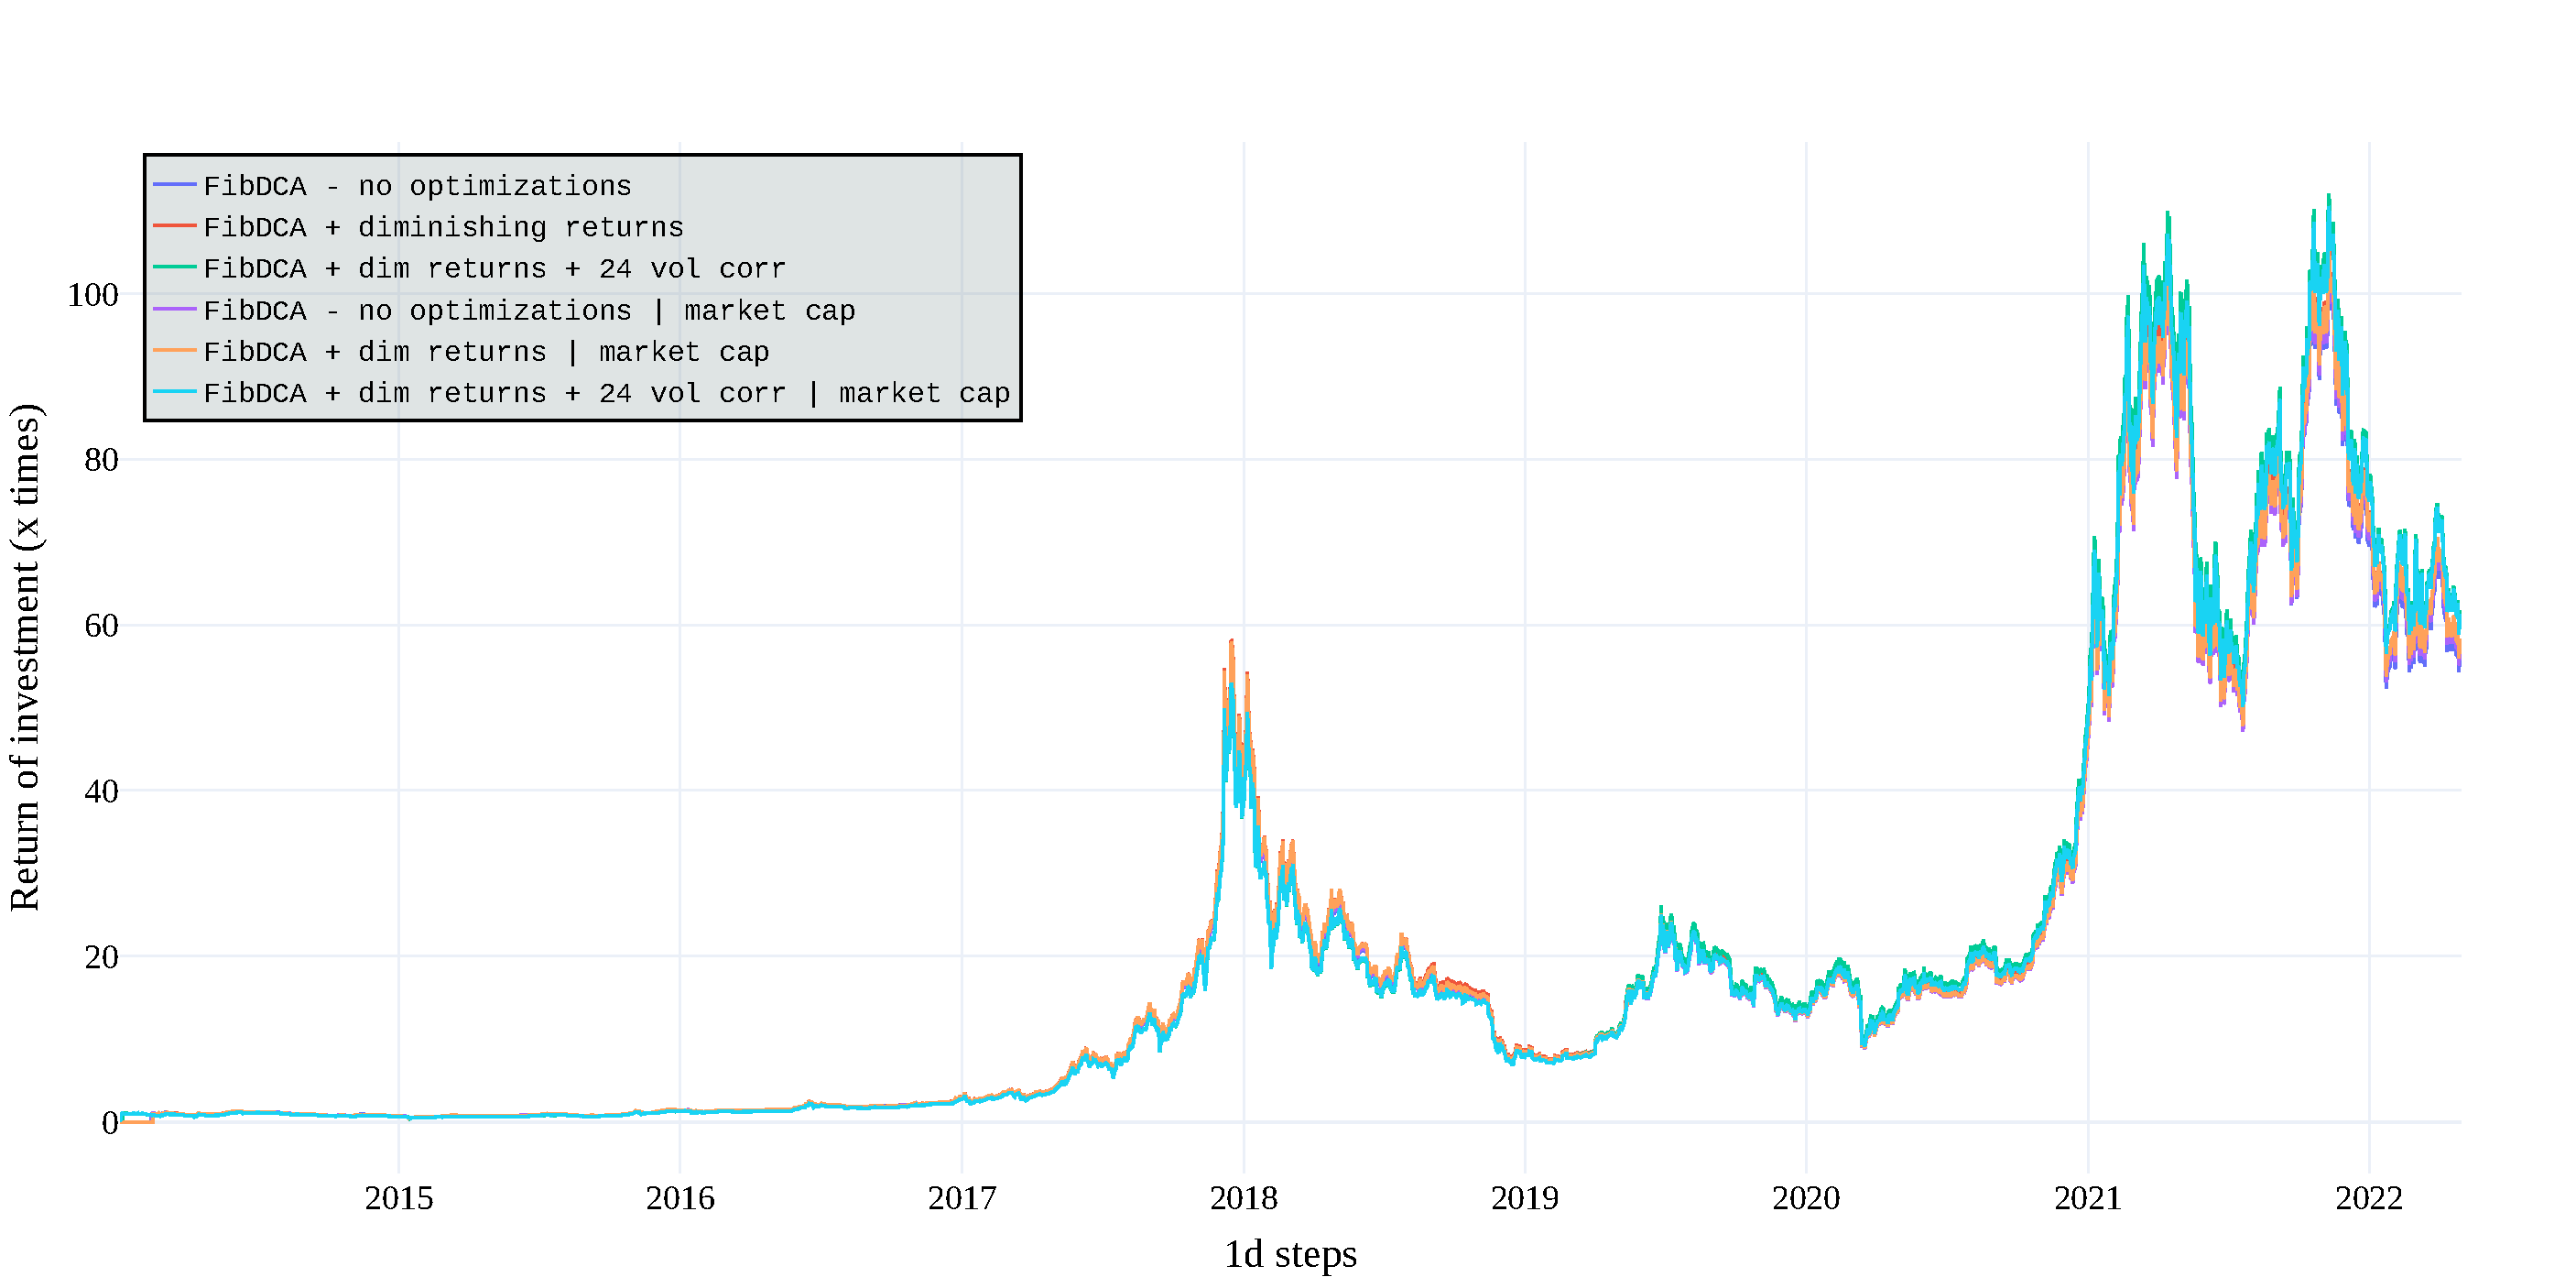
\includegraphics[width=\columnwidth]{figures/evaluation-dca-optimization-longer.pdf}
    \caption{Comparison of risk optimizations used with the adjusted Fibonacci sequence DCA strategy, dates: Jan 2014--May 2022.}
    \label{figure-dca-optimization-longer}
\end{figure}

\begin{figure}[!t]
    \centering
    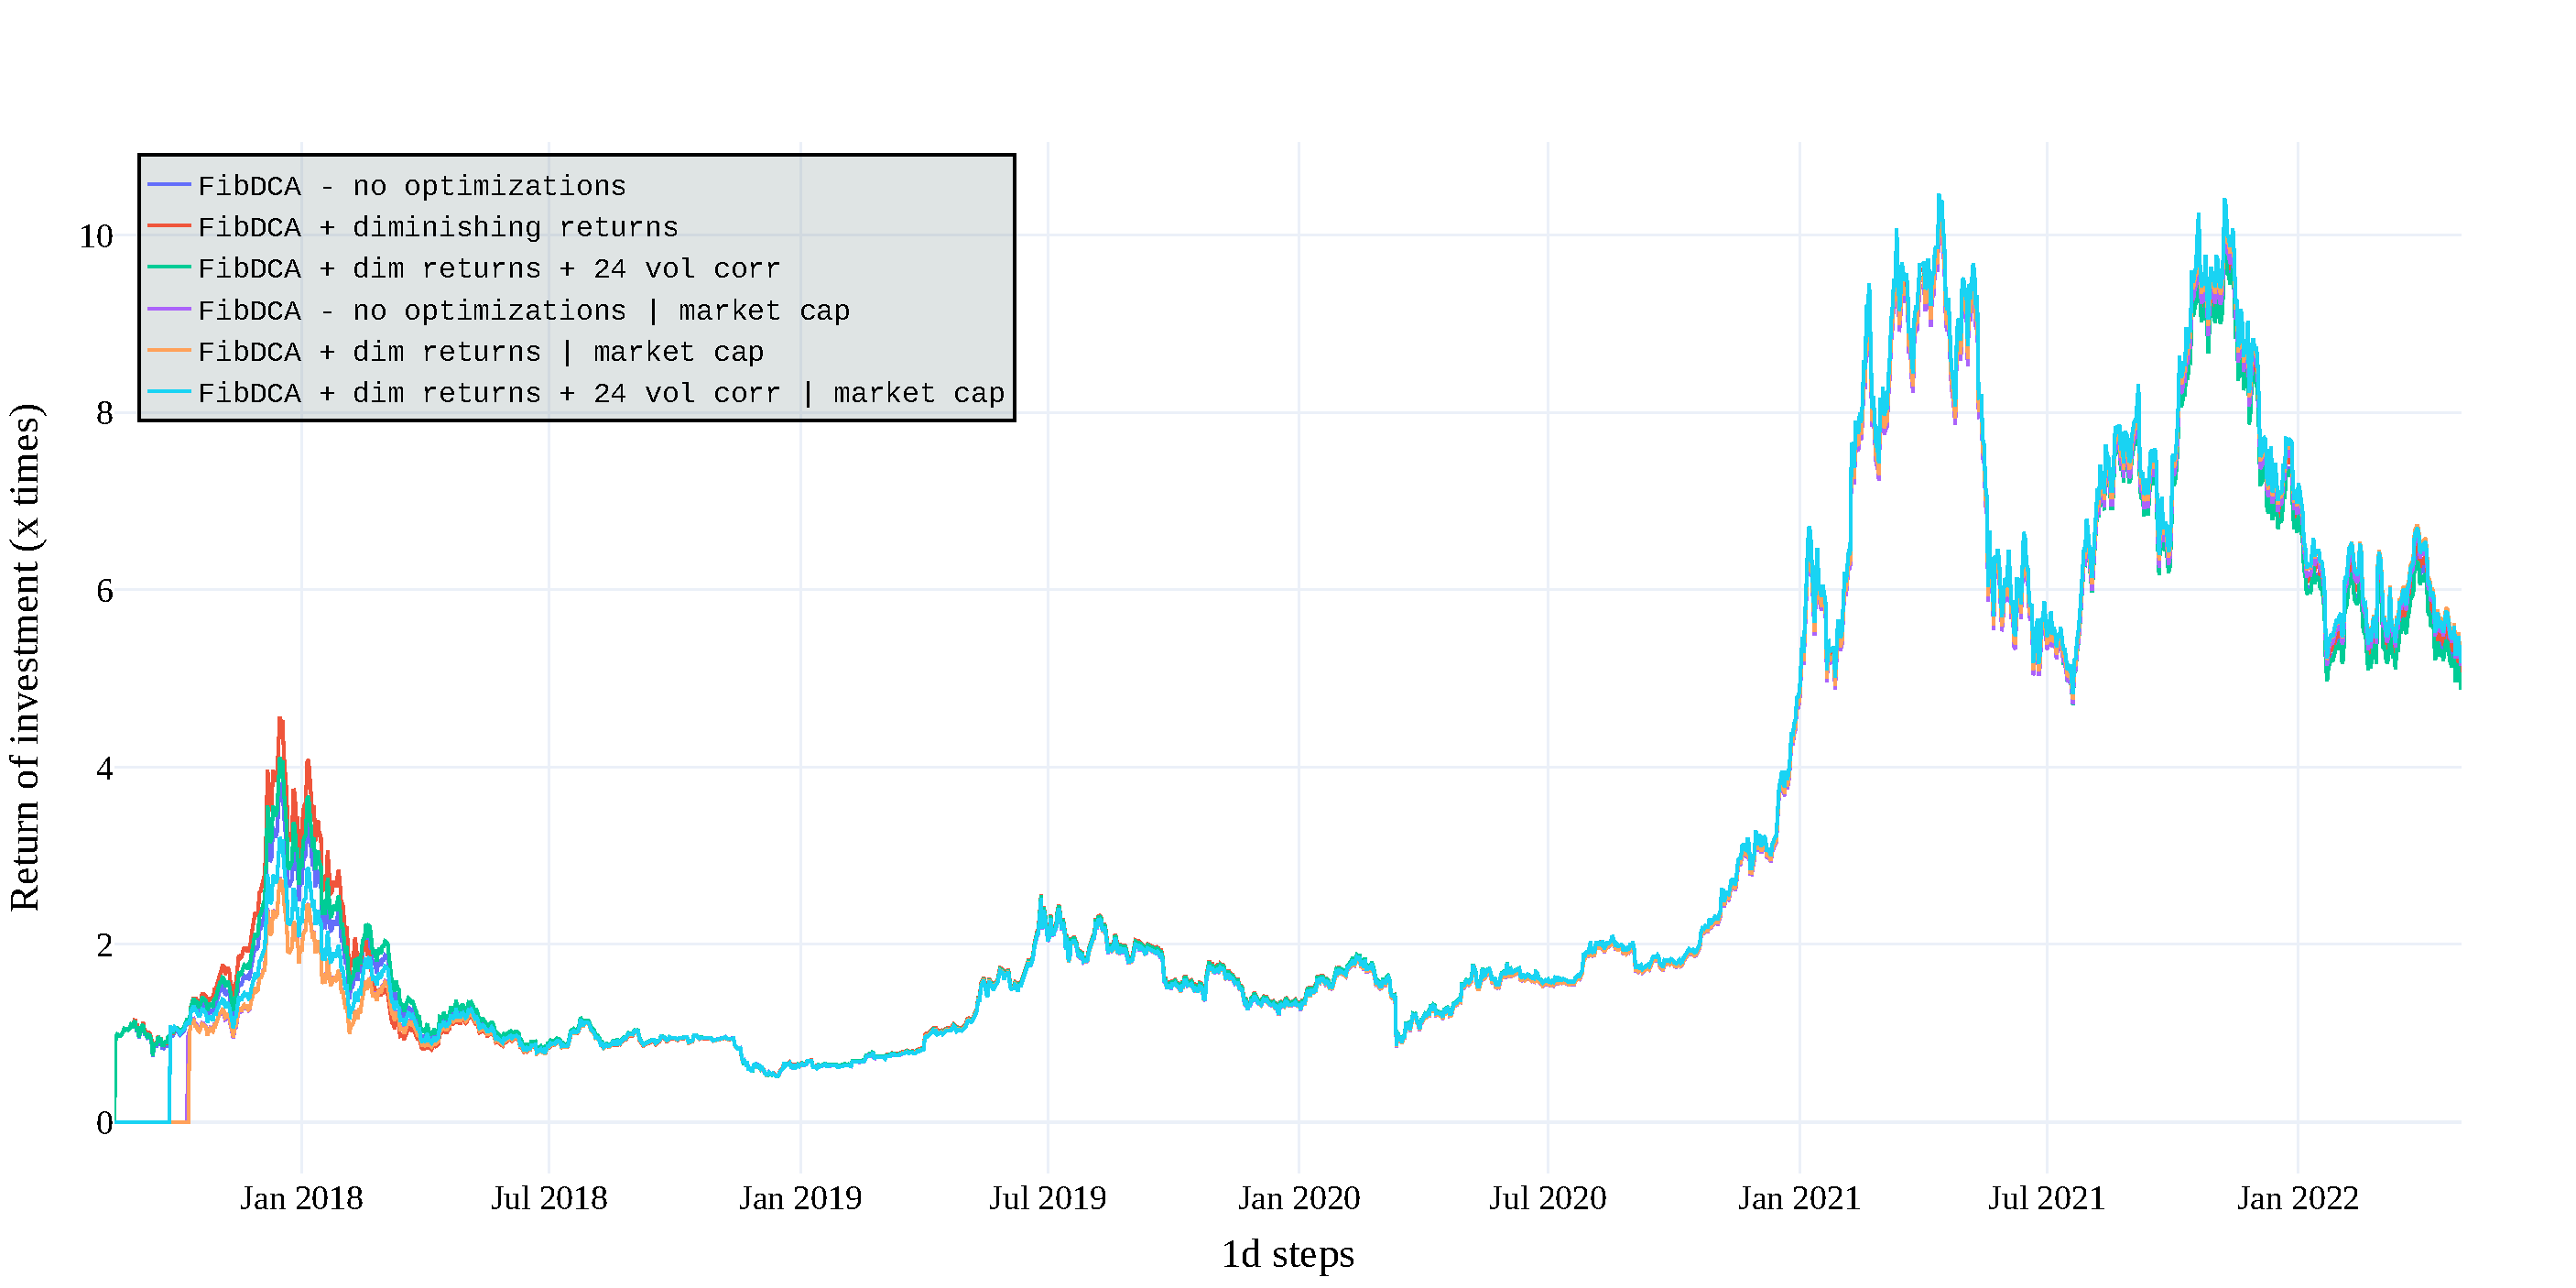
\includegraphics[width=\columnwidth]{figures/evaluation-dca-optimization-shorter.pdf}
    \caption{Comparison of risk optimizations used with the adjusted Fibonacci sequence DCA strategy. Dates: July 2017--May 2022.}
    \label{figure-dca-optimization-shorter}
\end{figure}

Firstly, in contrast with the previous results, the daily volume correlation seems promising in the results. Although, the overall results seem inconsistent when the longer and shorter data ranges are compared. And surprisingly, total market capitalization seems to be a better indicator in some cases.

If an optimal combination should be chosen, the diminishing returns optimization together with daily volume correlation applied on total market capitalization data seem to be the most consistent. When only looking at the historical Bitcoin data, diminishing returns optimization seems to be the one that is the most consistent.

If the results from the previous DCA return of investment, mentioned in Section~\ref{subsection-eval-dca}, should be compared with the new optimizations, the results would be as follows. The diminishing returns optimization paired together with daily volume correlation, and applied on total market capitalization has return of investment of $59.6$ times the original. That is just over 8\% better than the previous DCA results.

\section{Working With Portfolios of Many Coins}
We implemented the adaptive strategies. We defined the optimal evaluation strategies. We found the perfect risk combinations to go with these strategies. But all these simulated only one cryptocurrency---Bitcoin. This Section focuses on simulating many coins, how are the results compared to previous findings and the traditional rebalance approach described in Section~\ref{section-rebalance}.

\subsection*{Choosing the Coins}
Two portfolios are used for the evaluation. Portfolio A~is using only the Bitcoin and Ethereum, these two assets show promising and stable growth and have been the 2 biggest contributors to total market capitalization. As of May 1st 2022, the two cryptocurrencies contribute to almost 62\% of total market capitalization~\cite{coinmarketcap:globalmetrics}. Both cryptocurrencies of the portfolio date back to the earliest Binance data point, 17th August 2017.

For portfolio B, many more coins are chosen. The top 18 coins (not tokens) listed on the CoinMarketcap~\cite{coinmarketcap}, based on market capitalization and disregarding stablecoins, have been chosen. The coins have been chosen not only by the current day, but I~made sure they were at least somewhat popular during the two previous years. The overall age of the portfolio is much younger, only dating back to 2020. The difference between the portfolios should show how the strategies change depending on the portfolio size and disparity.

Assets (tickers) of the portfolio A:
\begin{itemize}
    \item Bitcoin (BTC)
    \item Ethereum (ETH)
\end{itemize}
The Longest possible date range of the portfolio A: 17th July 2017--today

Assets (tickers) of the portfolio B:
\begin{itemize}
    \item Bitcoin (BTC)
    \item Ethereum (ETH)
    \item XRP
    \item Cardano (ADA)
    \item Polkadot (DOT)
    \item Litecoin (LTC)
    \item BNB
    \item Bitcoin Cash (BCH)
    \item Avalanche (AVAX)
    \item Terra (LUNA)
    \item Monero (XMR)
    \item Stellar (XLM)
    \item Tron (TRX)
    \item NEAR Protocol (NEAR)
    \item Cosmos (ATOM)
    \item Algorand (ALGO)
    \item Polygon (MATIC)
    \item Solana (SOL)

\end{itemize}
Longest possible date range of portfolio B: 14th October 2020--today (limited by the NEAR Protocol)

\subsection*{Local Extrema Evaluation Strategy}
Like in the previous Section~\ref{section-sim-optimizations} we use the local extrema evaluation strategy. The diminishing returns optimization is simulated together with the market capitalization data option. Results for the portfolio A~are shown in Figure~\ref{figure-extrema-portfolio-A}.

\begin{figure}[!t]
    \centering
    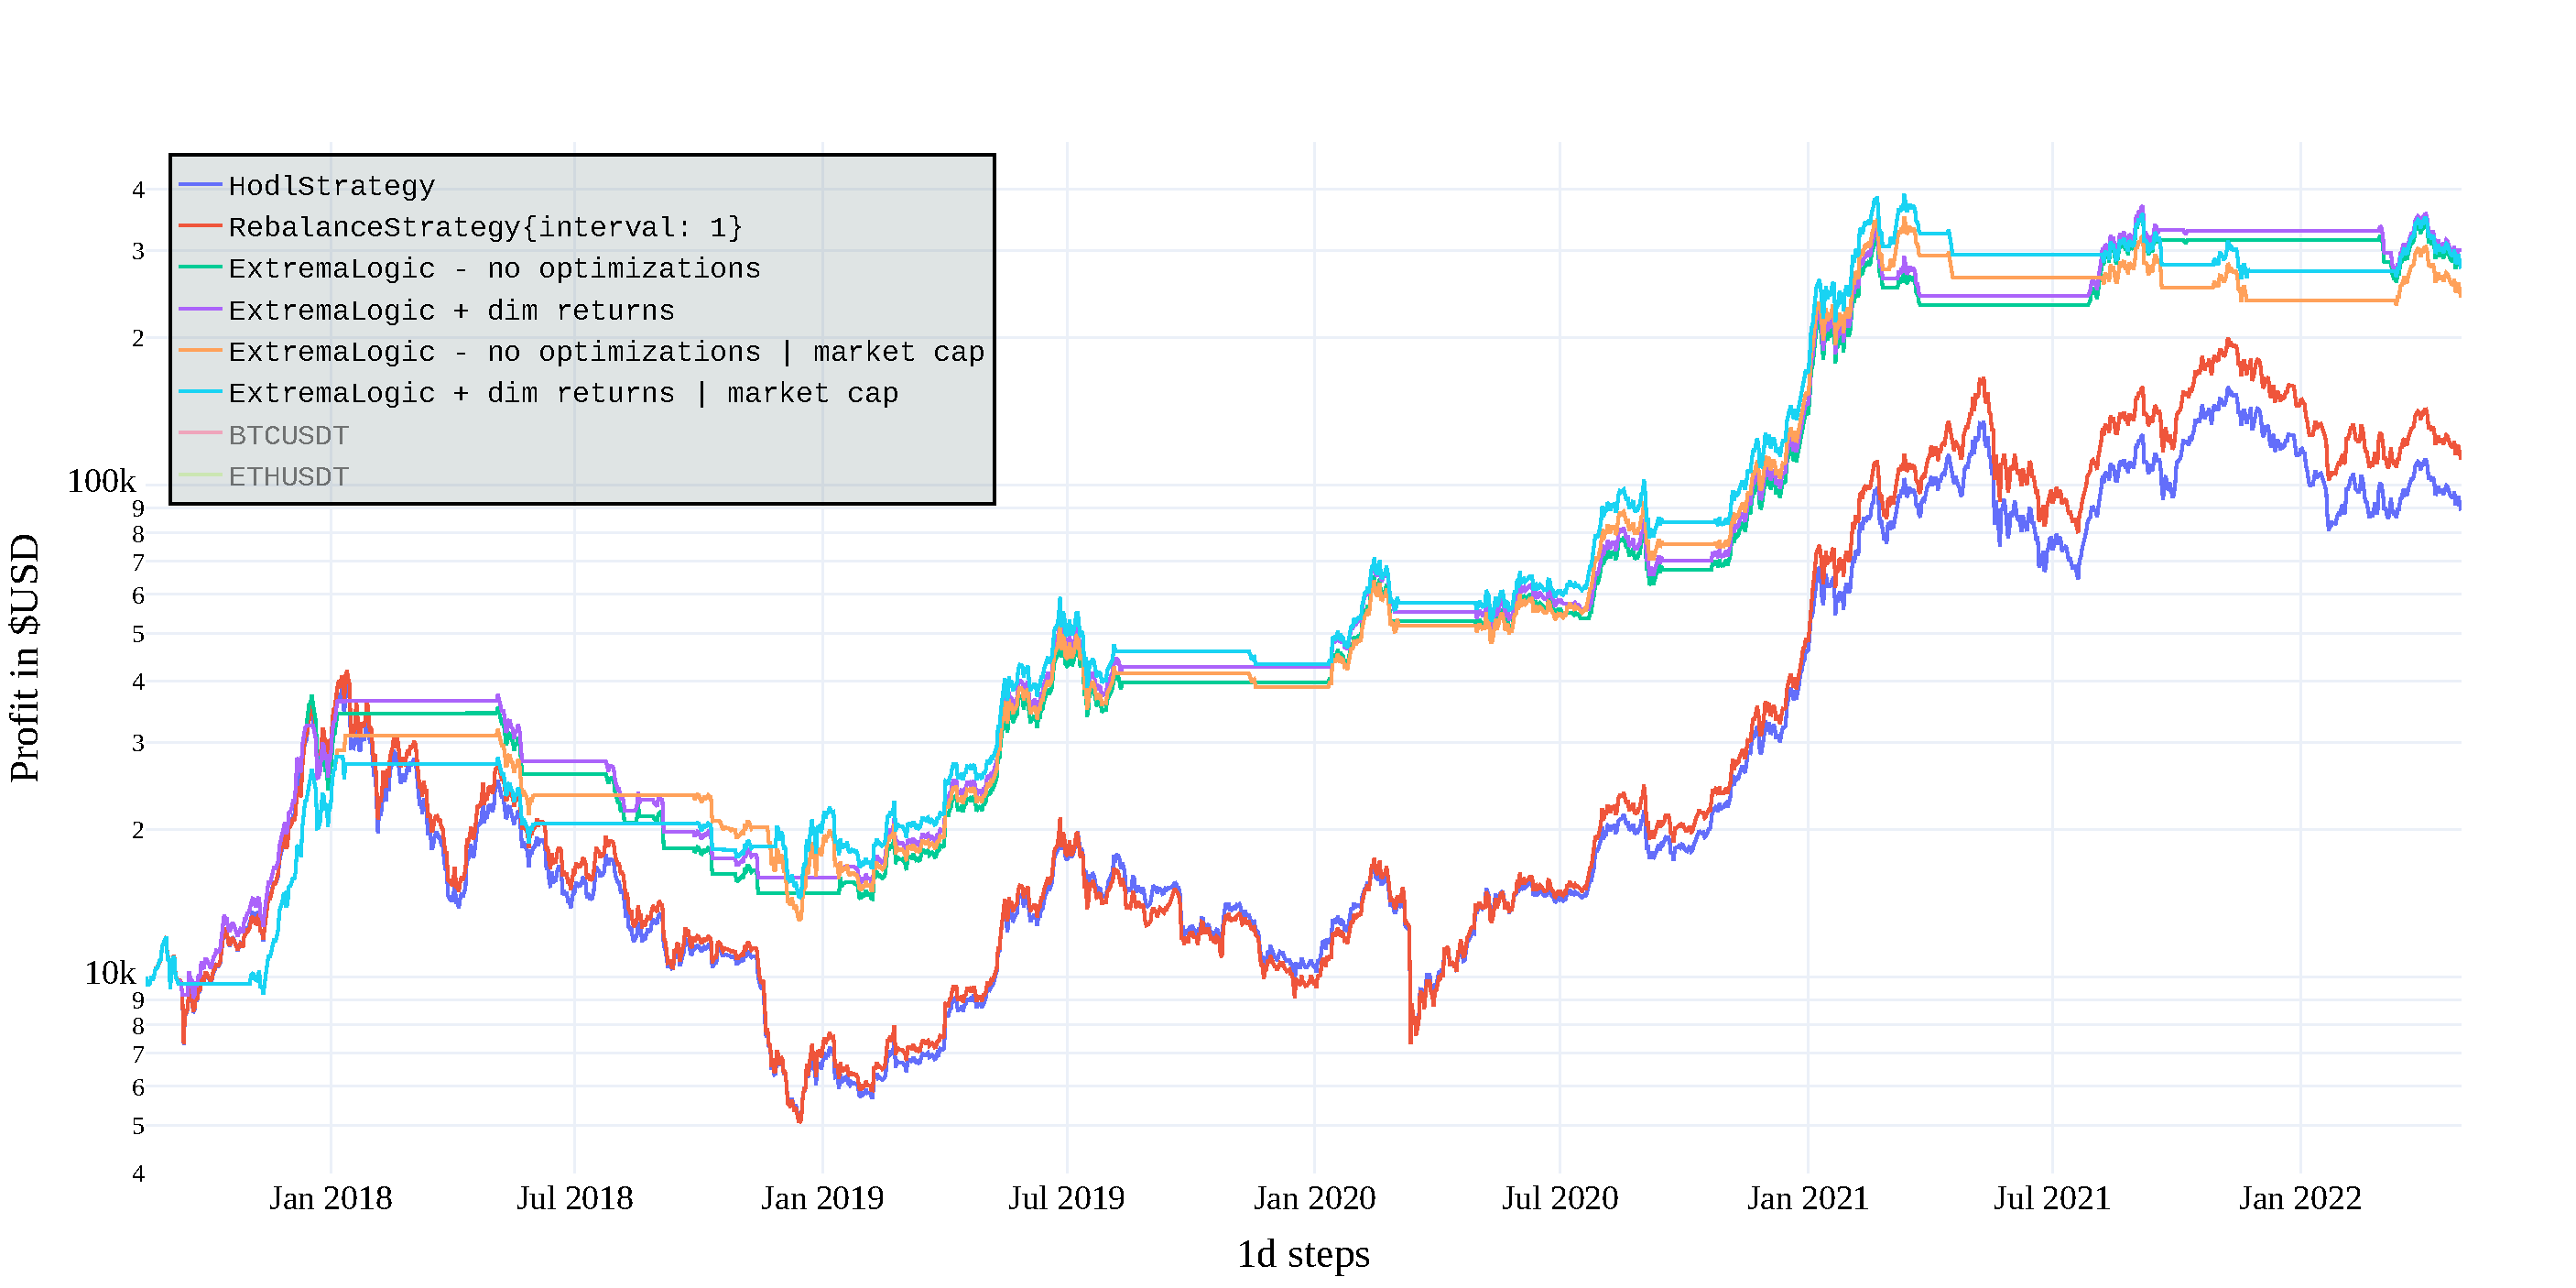
\includegraphics[width=\columnwidth]{figures/extrema-portfolio-A.pdf}
    \caption{Local extrema evaluation strategy against portfolio A.}
    \label{figure-extrema-portfolio-A}
\end{figure}

The results look similar as when testing with Bitcoin only. Diminishing returns optimization seems to dominate the charts again, and using total market capitalization data does not seem to bear any importance. The best strategy ended up with a bit over \$120,000. That is actual \$7,000 more than we ended up when testing the strategy on Bitcoin only. When looking at the performance, the best strategy was more than 3 times more performant than HODL and little bit less than 3 times performant than rebalance.

The results for portfolio B, shown in figure~\ref{figure-extrema-portfolio-B}, look very underperforming. Interestingly, even rebalance performs worse than HODL. HODL's profit si more than double compared to the other strategies. It looks like the strategy does not have enough time to really get accustomed to the market. Some shorter-term strategy may be more interesting in this case.

\begin{figure}[!t]
    \centering
    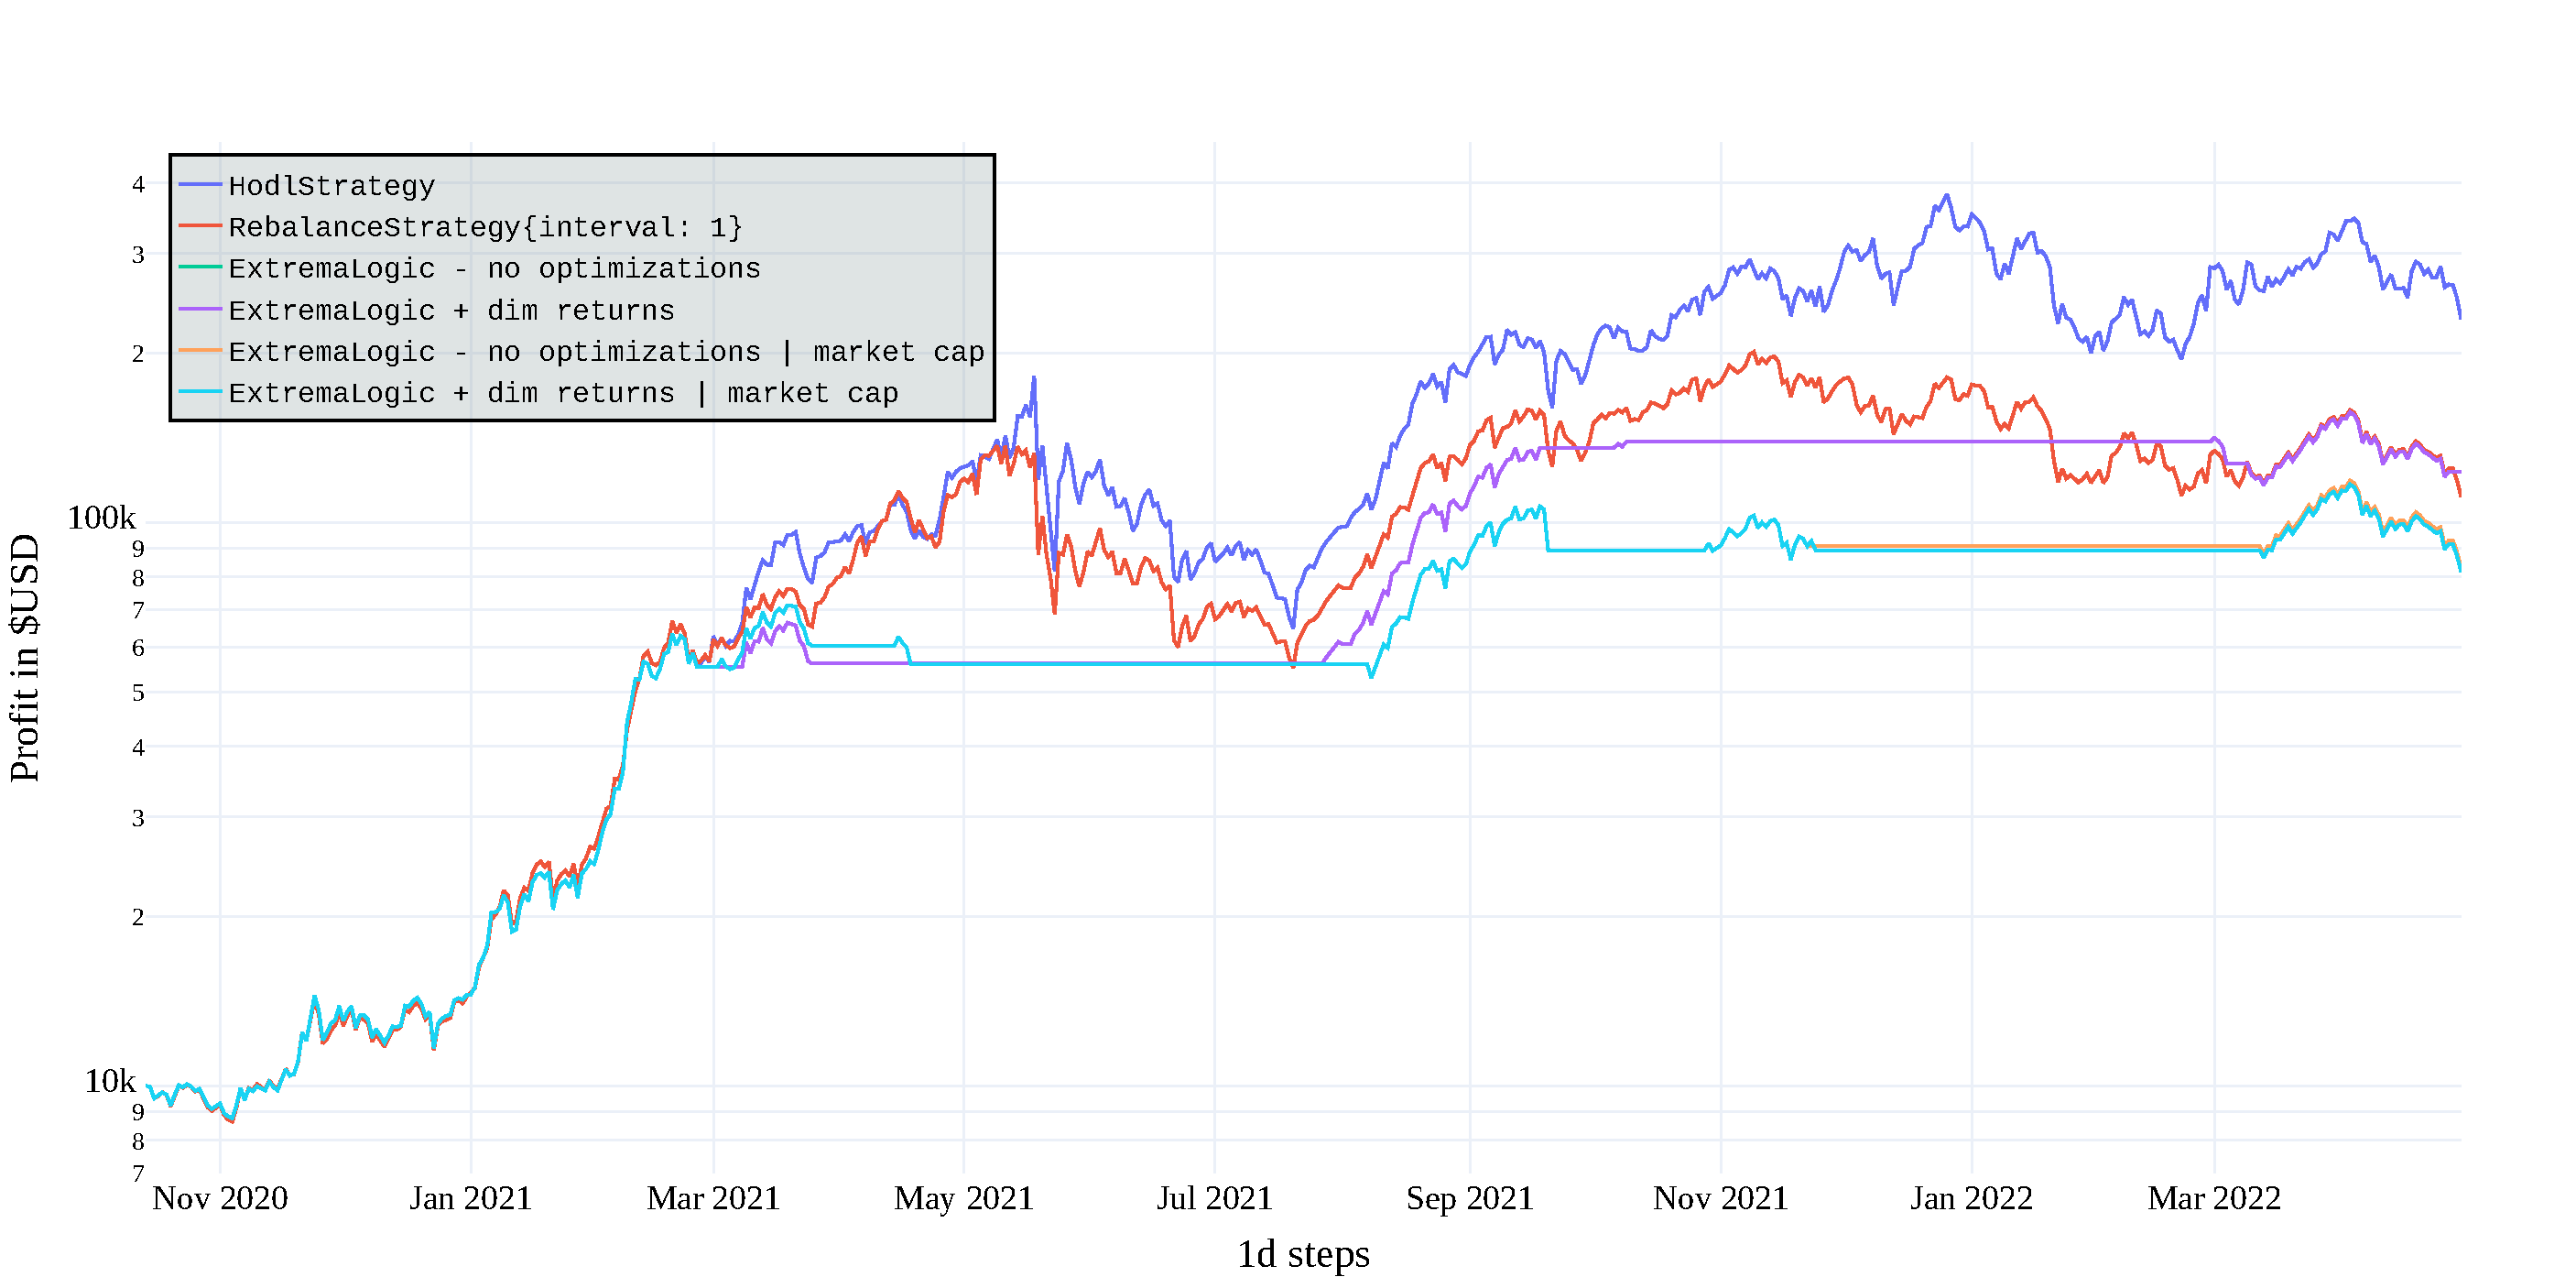
\includegraphics[width=\columnwidth]{figures/extrema-portfolio-B.pdf}
    \caption{Local extrema evaluation strategy against portfolio B.}
    \label{figure-extrema-portfolio-B}
\end{figure}


\subsection*{Adjusted Fibonacci Sequence DCA Strategy}
Similarly, as in the previous Section~\ref{section-sim-optimizations} we use the adjusted Fibonacci sequence DCA (dollar-cost averaging) strategy. The diminishing returns optimization and daily volume correlation is simulated together with the market capitalization data option. Results for portfolio A~are shown in Figure~\ref{figure-fibseq-portfolio-A}.

\begin{figure}[!t]
    \centering
    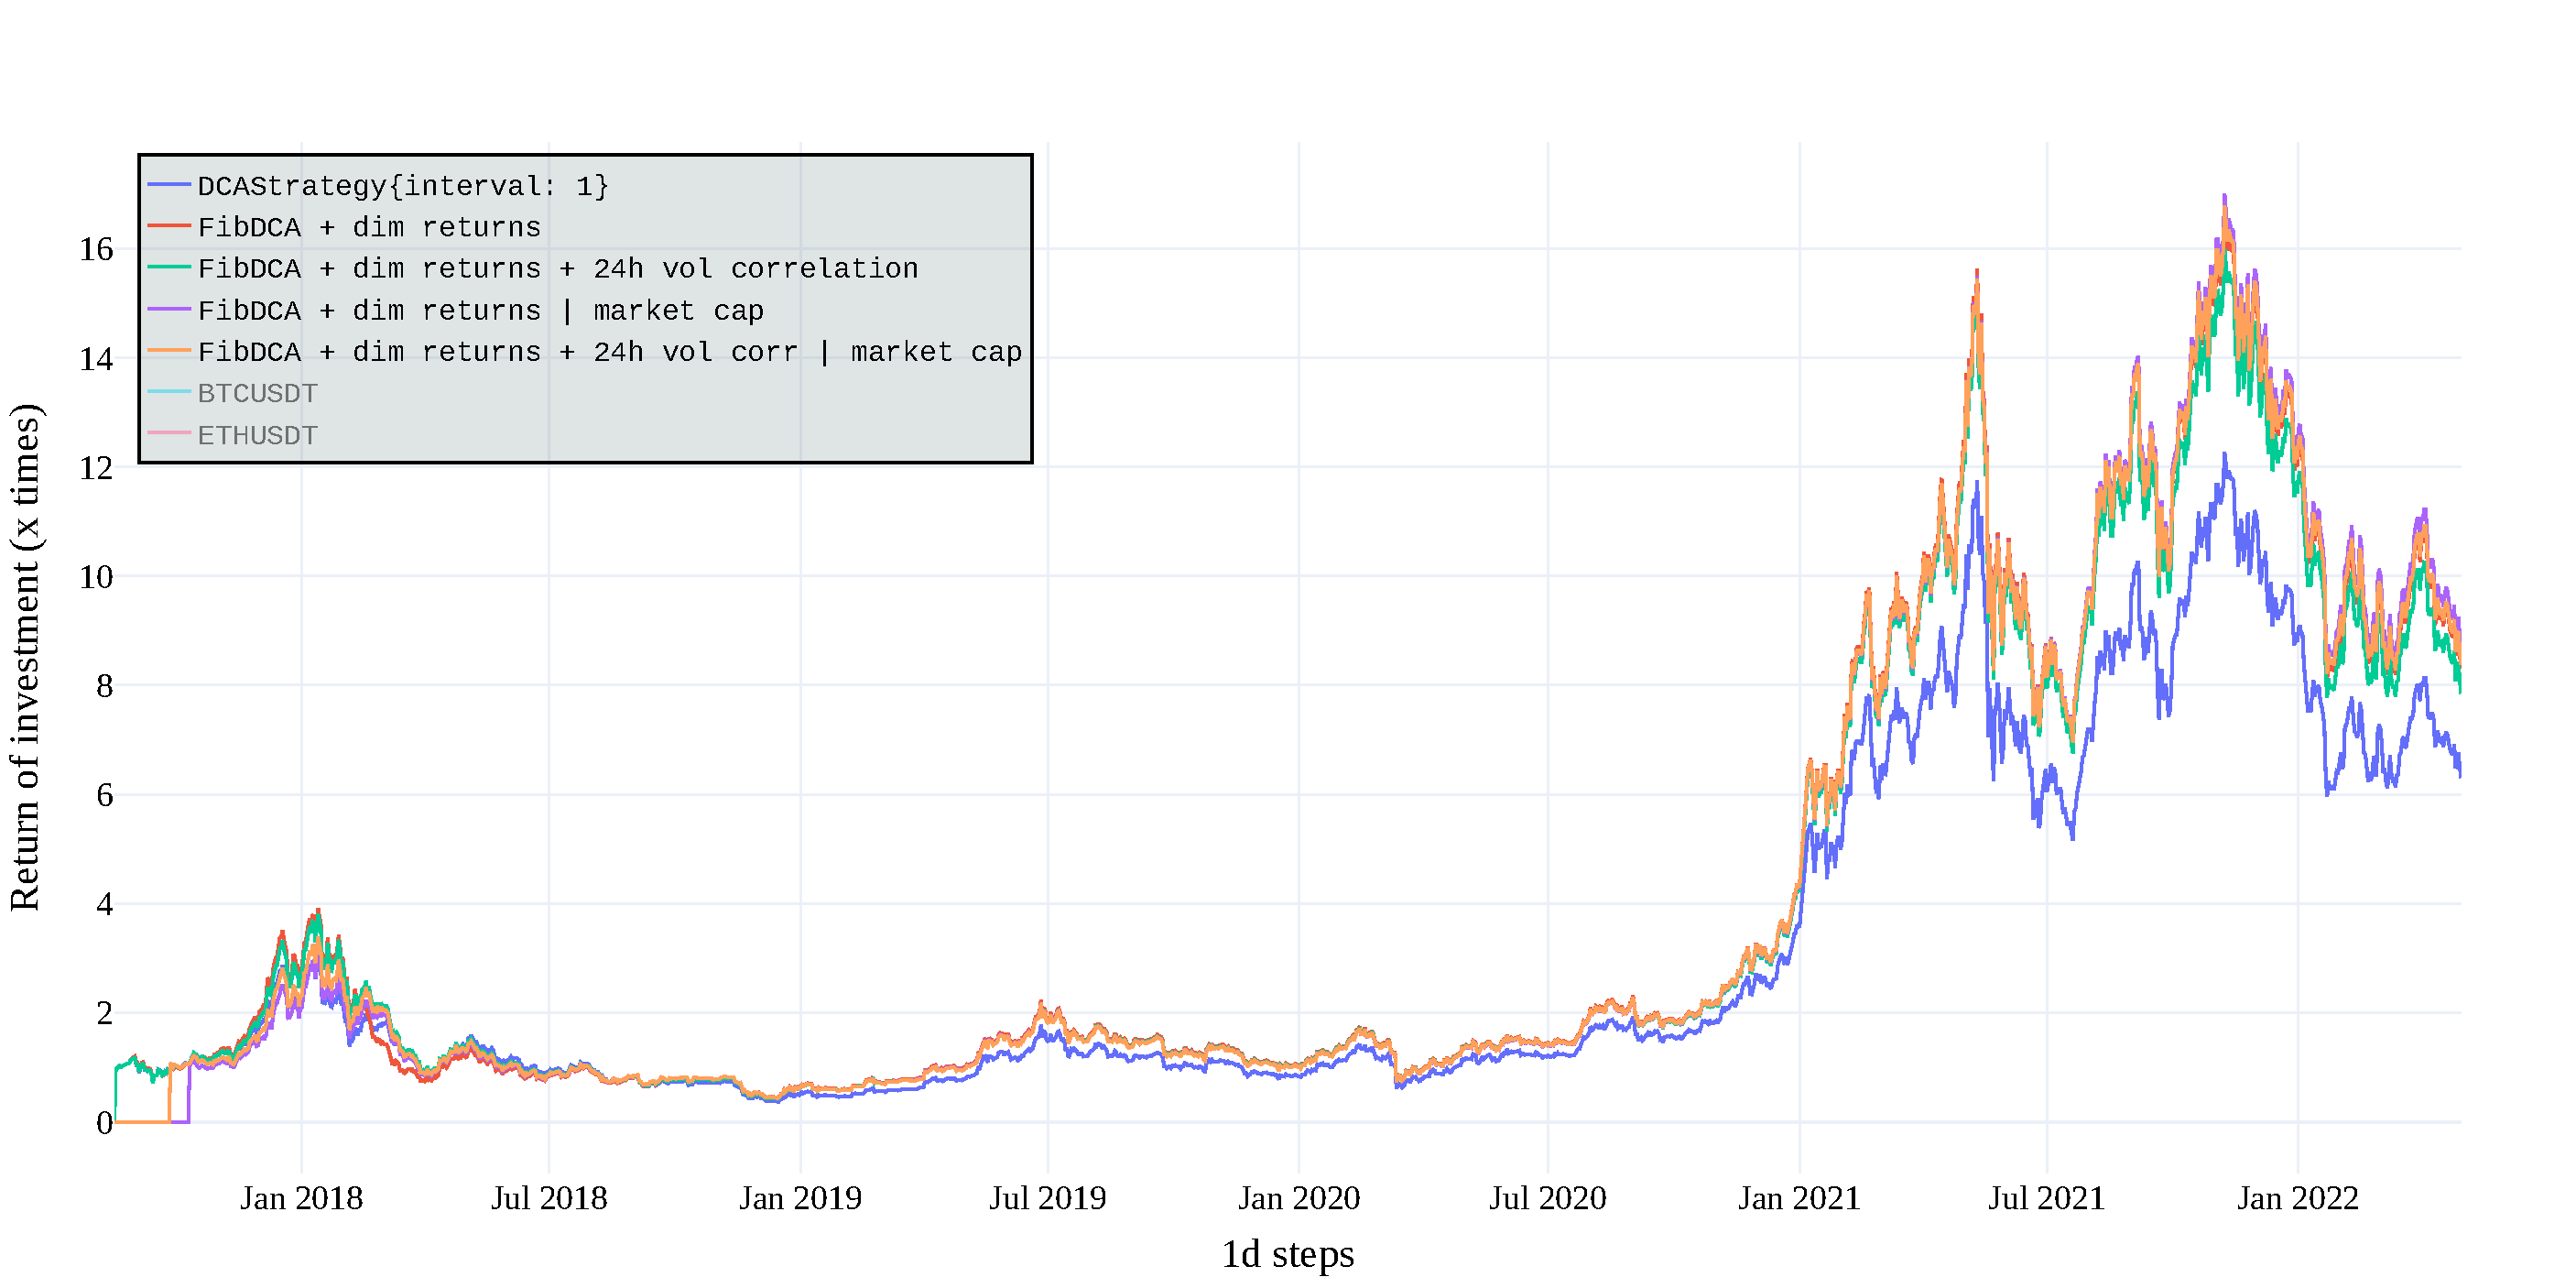
\includegraphics[width=\columnwidth]{figures/fibseq-portfolio-A.pdf}
    \caption{Adjusted Fibonacci sequence DCA strategy against portfolio A.}
    \label{figure-fibseq-portfolio-A}
\end{figure}

Using market capitalization data for the DCA here looks to be beneficial as before. The best strategy outperformed the classic DCA strategy by almost 37\%. That result is comparable to the findings of Section~\ref{subsection-eval-dca}.

The results for portfolio B can be seen in figure~\ref{figure-fibseq-portfolio-B}. Here an interesting phenomenon occurs. The risk-adjusted strategies gain a huge profit from March to May 2021, but then they slowly begin to lose it all the way until the classic DCA outperforms by the end of April 2022. This shows that more extensive research should be done when trading with many coins with the proposed strategies.

\begin{figure}[!t]
    \centering
    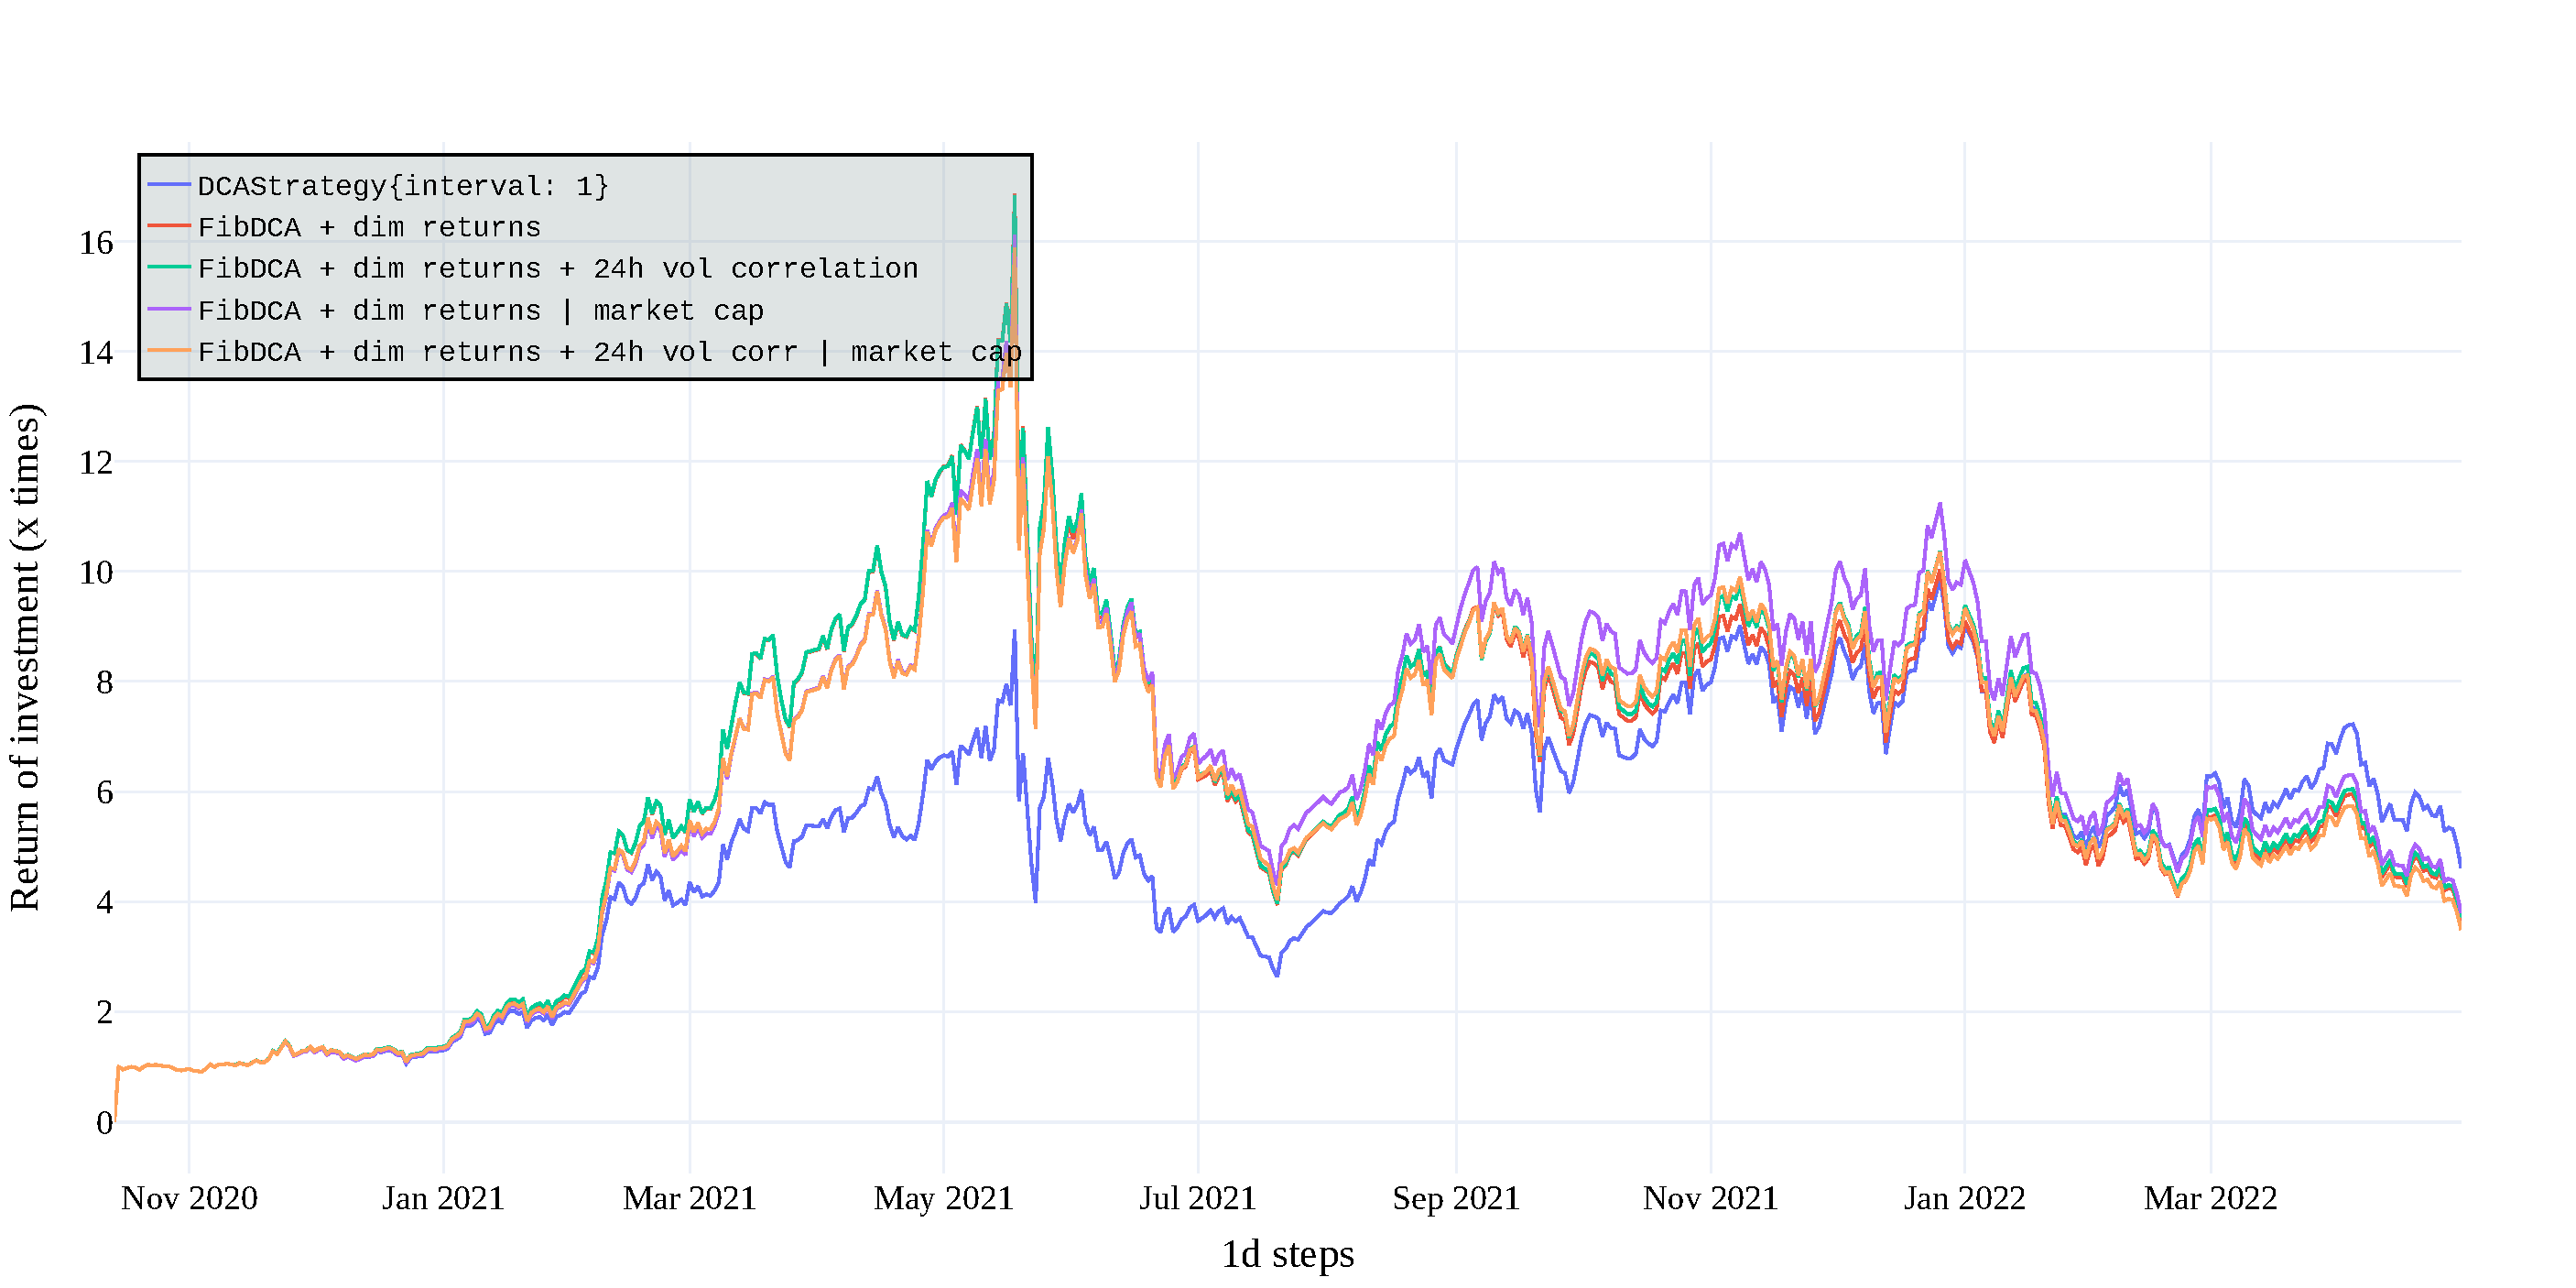
\includegraphics[width=\columnwidth]{figures/fibseq-portfolio-B.pdf}
    \caption{Adjusted Fibonacci sequence DCA strategy against portfolio B.}
    \label{figure-fibseq-portfolio-B}
\end{figure}

\section{Simulating Short-Term Trading}
\label{section-testing-day-trading}
When focusing on short-term trading, range trading and scalping discussed in Sections~\ref{section-range-trading} and~\ref{section-scalping} respectively. We try to guess the support and resistance levels.

When talking about technical analysis, we need to make support and resistance levels into an account. They can be predicted in several ways. Round numbers are taken into account, like \$50 and \$100, since investors usually put stop orders at such whole number points. These points then serve as resistance levels, since it takes a very large number of purchases to absorb the sales. Moving average can be used to estimate the levels, too, as you can see in the Figure~\ref{figure-ma-support-resistance}. Other indicators include the golden ratio, number of touches and others. This paragraph has been inspired by the Investopedia article~\cite{investopedia:support-and-resistance}, where more detailed information can be found.

\begin{figure}[!t]
    \centering
    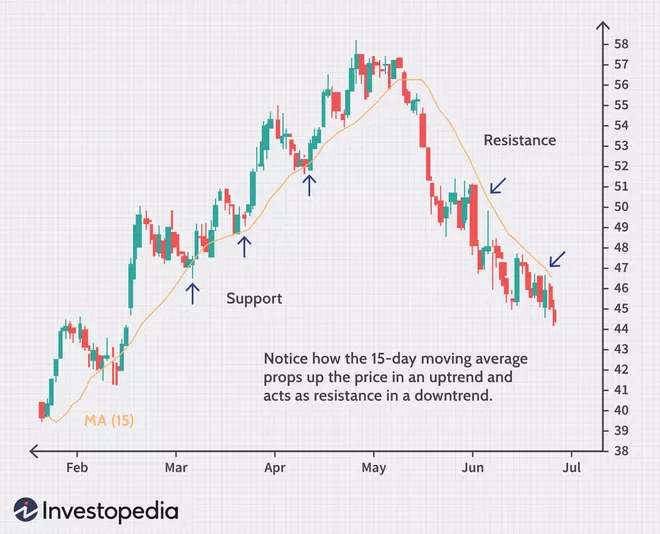
\includegraphics[width=\columnwidth]{figures/ma-support-resistance.png}
    \caption{Expected support and resistance levels computed by a moving average. Attribution: Investopedia~\cite{investopedia:support-and-resistance}.}
    \label{figure-ma-support-resistance}
\end{figure}

Optimizing for long term investing is great, it has a lower risk than trading throughout the day while still keeping good profits. But one thing it cannot do is to gain capital fast, that is where day trading can shine. In this section, the adaptive strategies are tested on a few several days window with 5 minute OHLCV portfolio data.

\subsection*{Creating the Strategy}
Instead of looking for long moving averages of 50 weeks and days as before, we will look at a different indicator. Moving average of 6 hours---that means 72 ticks of 5 minute data---is used as the metric. The moving average smooths out the rigidity of the 5-minute data and allows us to exploit the rising and falling trends during the day. It is a form of range trading~\ref{section-range-trading} where we take advantage of the fact that cryptocurrencies fluctuate multiple times during a day.

\subsection*{Strategy Evaluation}
The strategy is simulated on Bitcoin only. It does not make much sense to test the strategies with many cryptocurrencies, because the strategy is tailored to one asset only. Theoretically, a portfolio with many cryptocurrencies can run this strategy individually per every currency.

The basic evaluation strategy is to sell at the local maxima of the moving average and buy at the local minima. Thus trying to buy low and sell high. The local maxima and minima take the 3 points from each side into consideration---this prevents too many extrema next to each other, which would not be useful. As before in Section \ref{subsection-local-extrema}, we need to readjust from the ideal point by several ticks, the drawback may be more significant here, as the data is much more volatile.

Three date range have been chosen to evaluate the results. A~date range with a falling, rising and changing trend. The results can be seen in Figures~\ref{figure-short-term-rising},~\ref{figure-short-term-falling} and~\ref{figure-short-term-changing}.

\begin{figure}[!t]
    \centering
    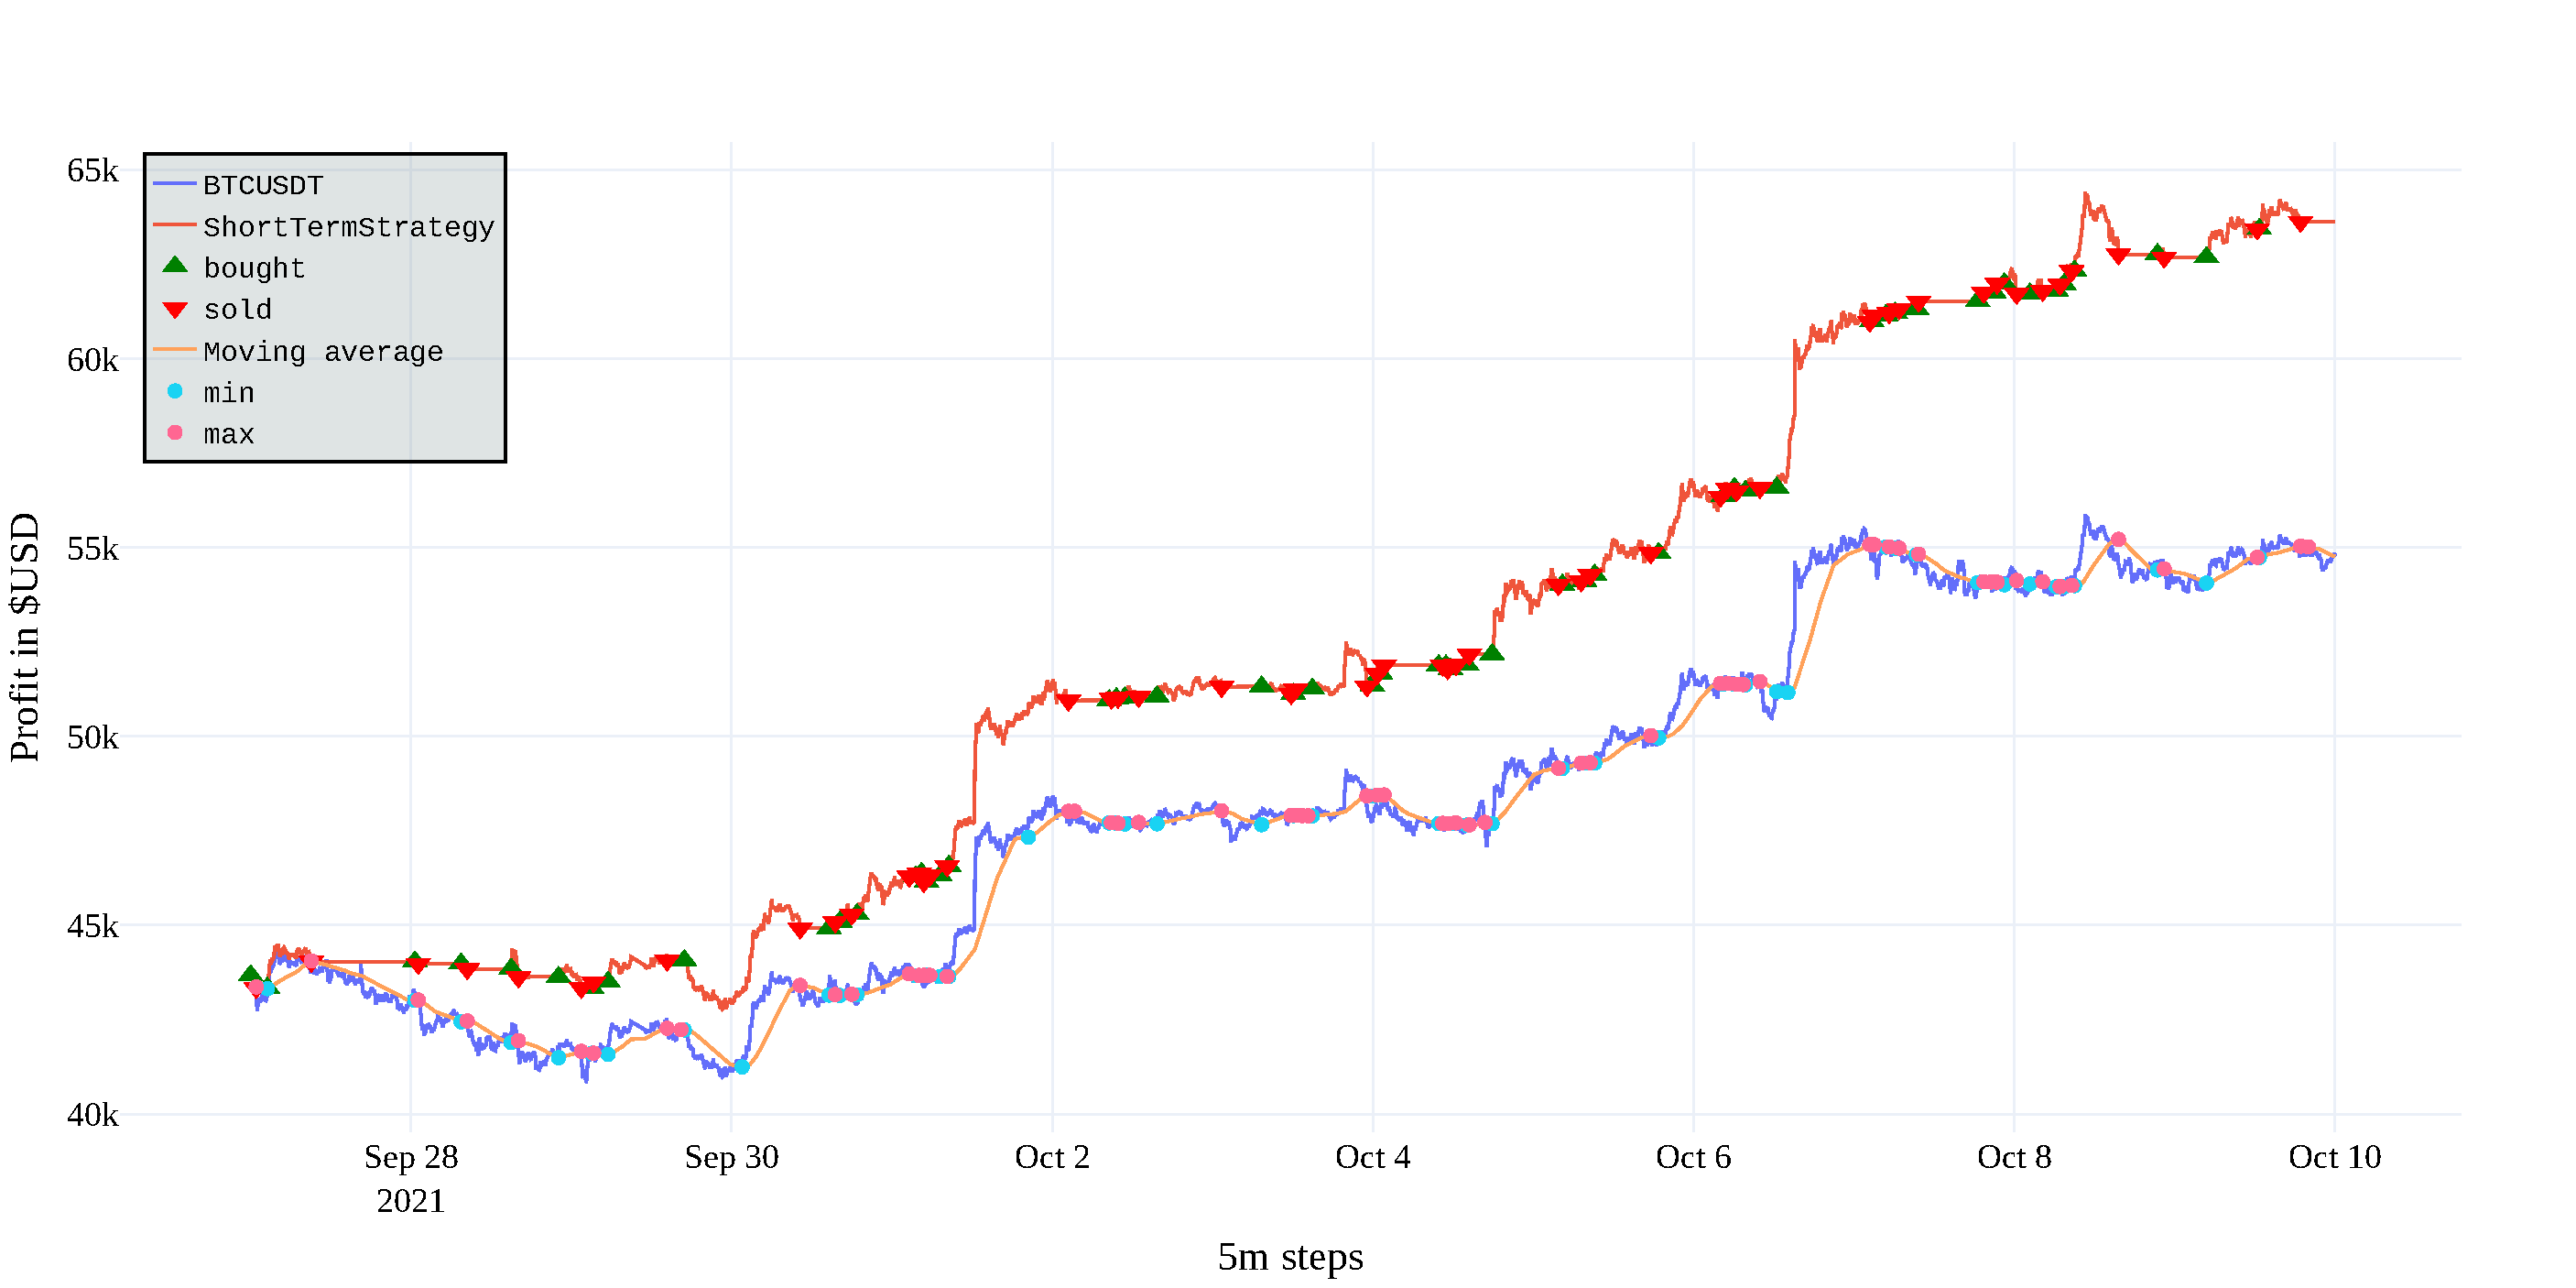
\includegraphics[width=\columnwidth]{figures/short-term-rising.pdf}
    \caption{27th Sep--10th Oct 2021 rising trend that registered rise from \$43000 to \$55000.}
    \label{figure-short-term-rising}
\end{figure}

\begin{figure}[!t]
    \centering
    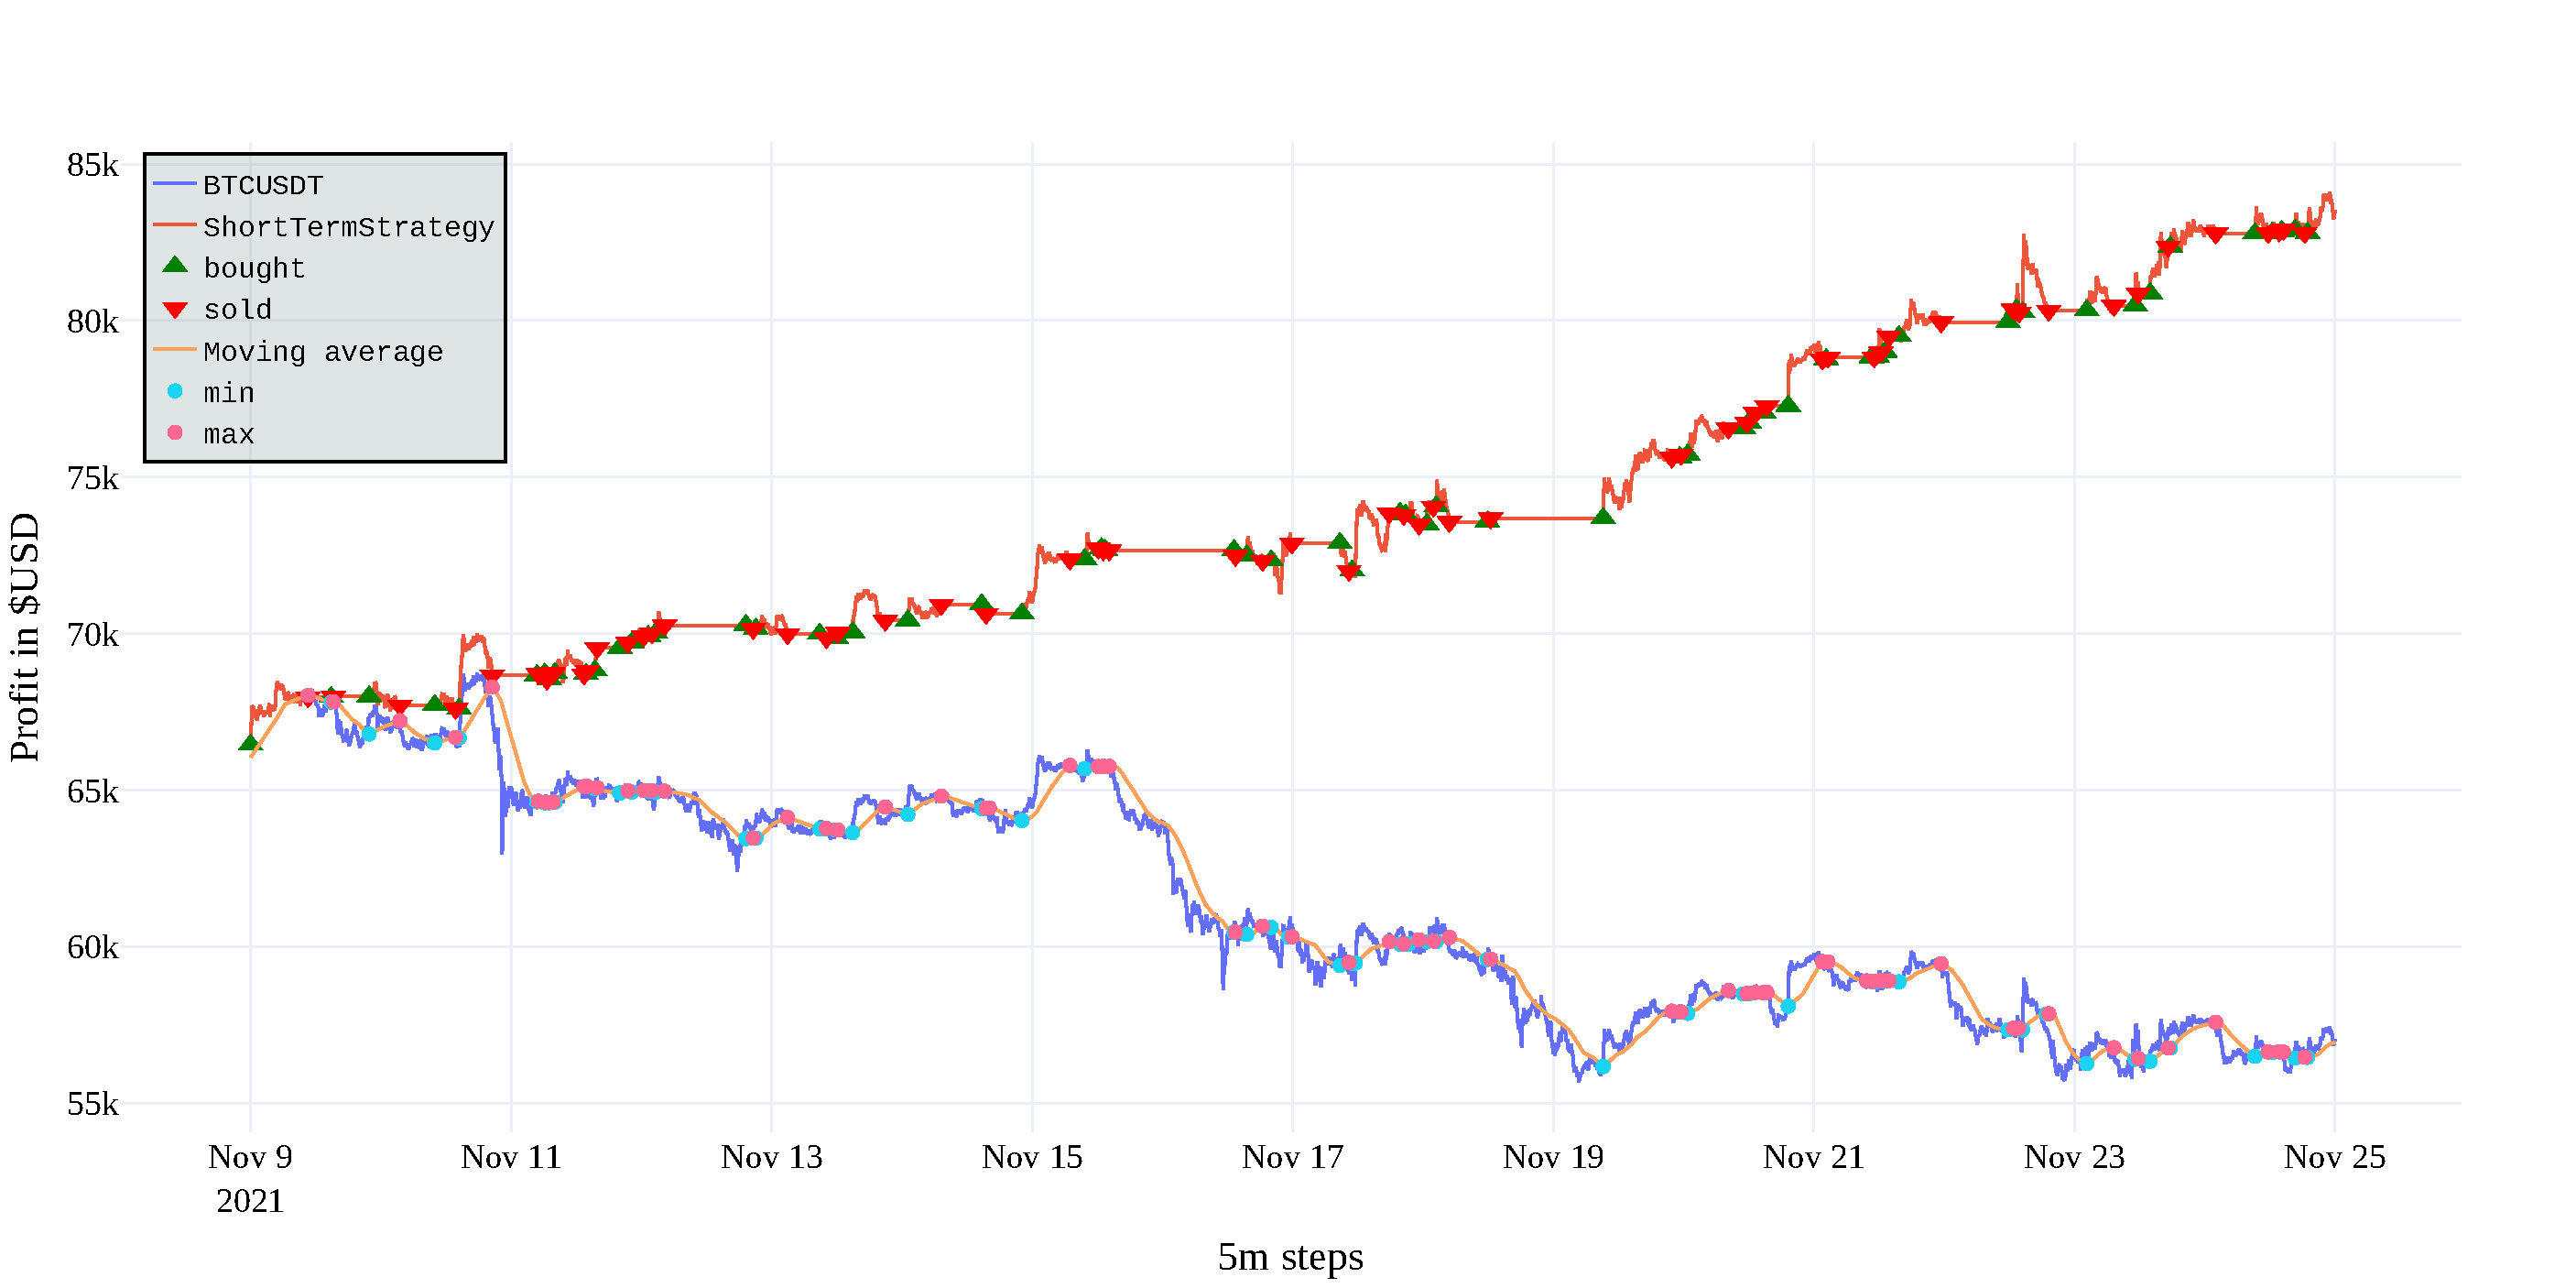
\includegraphics[width=\columnwidth]{figures/short-term-falling.pdf}
    \caption{9th Nov--25th Nov 2021 falling trend that registered fall from \$65000 to \$55000.}
    \label{figure-short-term-falling}
\end{figure}

\begin{figure}[!t]
    \centering
    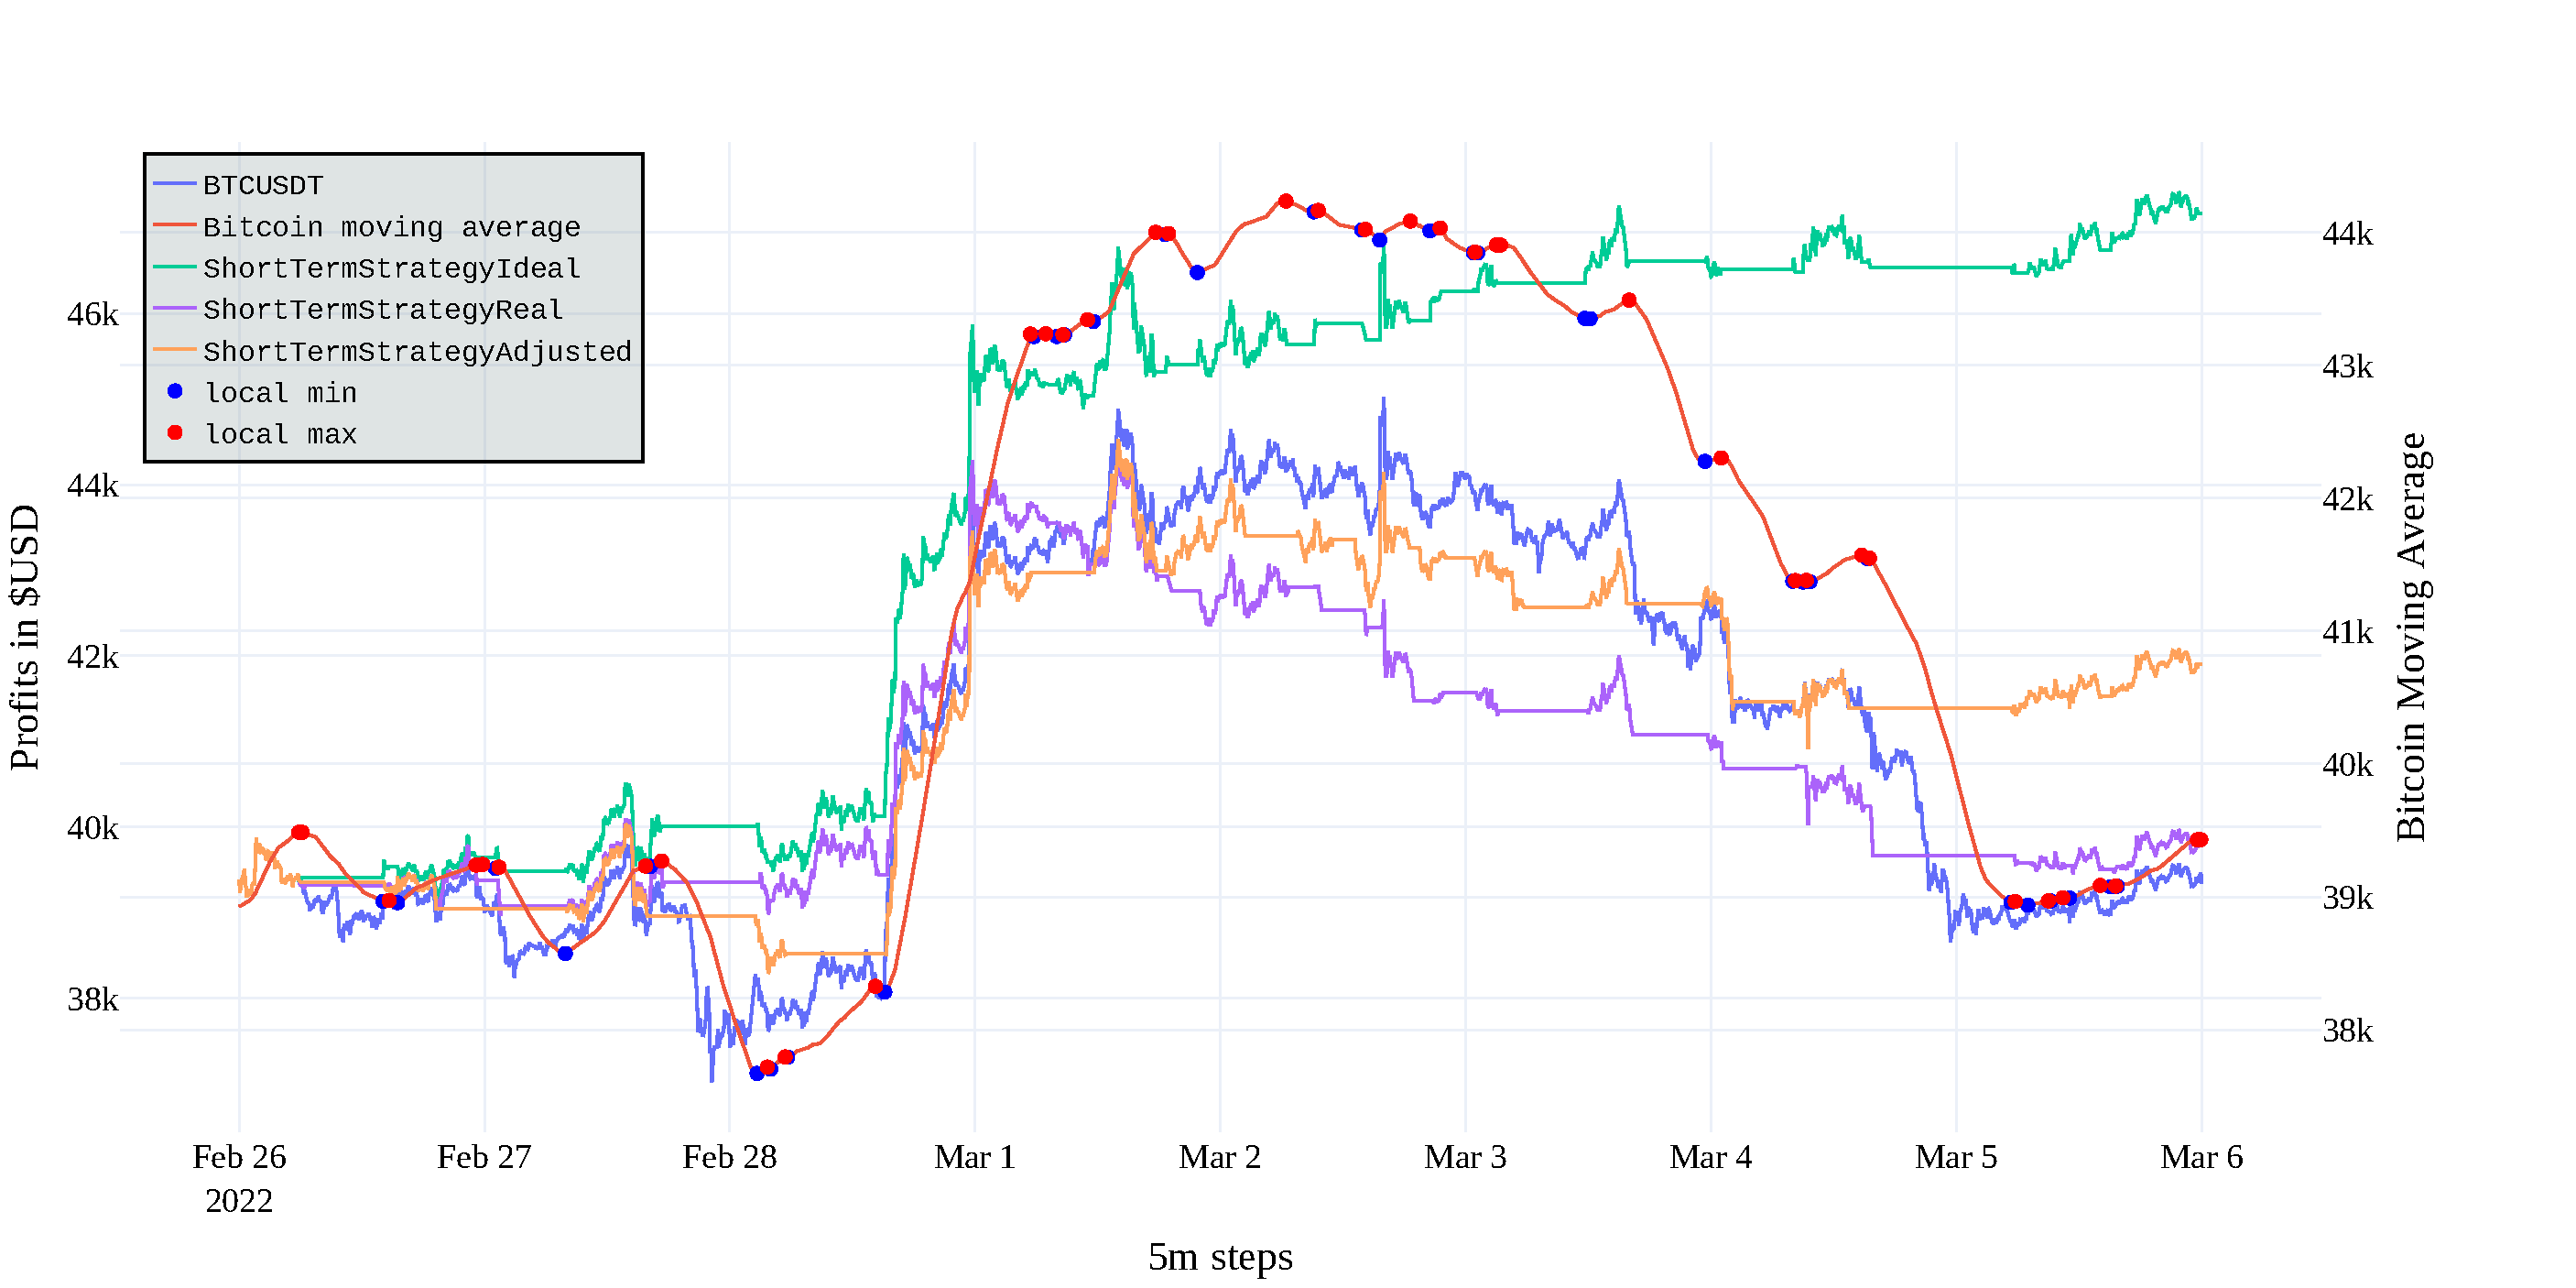
\includegraphics[width=\columnwidth]{figures/short-term-changing.pdf}
    \caption{26th Feb--6th Mar 2022 changing trend.}
    \label{figure-short-term-changing}
\end{figure}

As you can see, if the strategy was optimal and idealized, the profits would be very, very high. That is not the real case, and we must take the current day into consideration. The "ShortStrategyIdeal" show us idealized data, "ShortStrategyReal" show how that same metric would turn out with realistic extremes, and finally "ShortStrategyAdjusted" further plays with the previous strategy, disallowing sells that are too near of each other on the moving average.

The non-ideal strategies perform very poorly compared to the ideal one. We can see that the falling date range experiences the most profits. One thing must be mentioned, that would diminish even the ideal strategy a bit. Most of the individual trades generate a little profit that only accumulates over time--meaning that exchange fees would diminish the results by a noticeable amount, and should be taken into account when considering using the strategies. Slippage and spread can also influence the results, since market orders are not instantaneous, a disadvantage of short-term trading.

In all of the Figures, we can see a steady rise of the ideal strategy. In the rising trend, we see that the realistic strategies underperform by a few thousands dollars. In the falling trend the performance is similar to HODL, and in the changing trend the strategies outperform HODL by up to \$2,500. The results so far do not tell us too much reliable information.

Let us see how the strategy fares when applied over several months. The date range chosen is February until April of the year 2022. The results can be seen in~\ref{figure-short-term-long}. The profits here have accumulated a bit in the adjusted strategy, generating a profit of \$42,000 against HODL's \$38,200. A~profit of almost 10\%. That is not much when we take into account the possible drawbacks and questionable reliability of the method. The ideal strategy trends upwards in an almost linear fashion, quadrupling its value over the span of 3 months. In contrast to that, the strategy that would be used in practice instead of the ideal one, made worse profits than HODL, ending up at \$37,230.

\begin{figure}[!t]
    \centering
    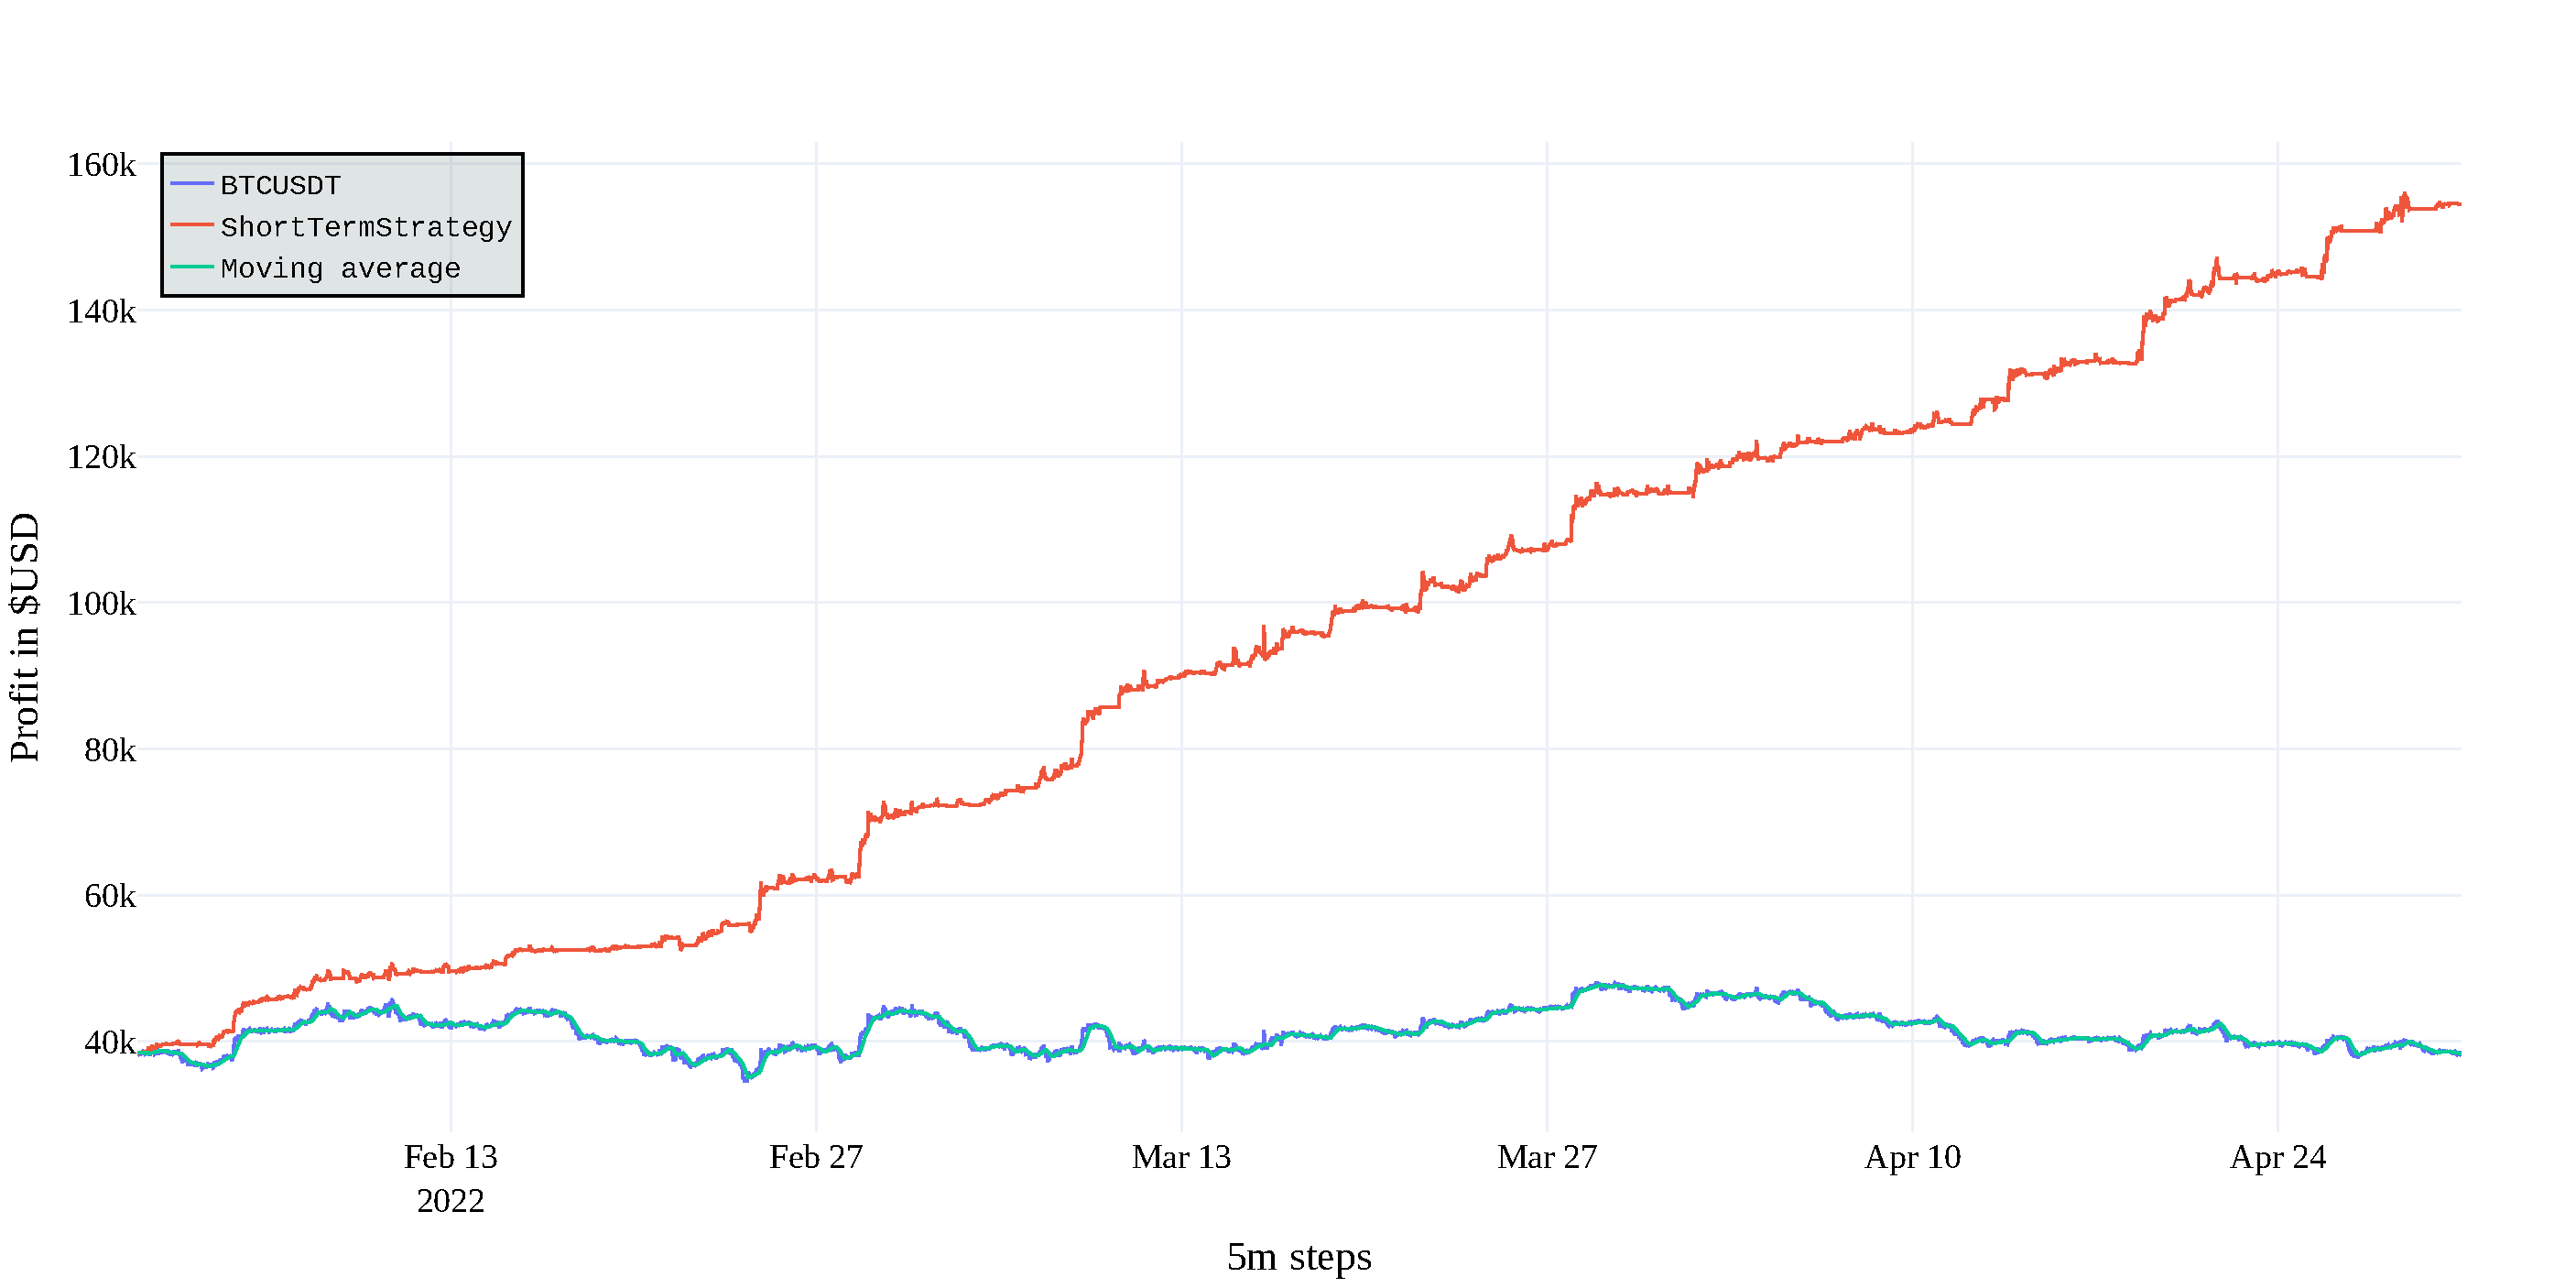
\includegraphics[width=\columnwidth]{figures/short-term-long.pdf}
    \caption{1st Feb--30th Apr 2022 long date range.}
    \label{figure-short-term-long}
\end{figure}

\section{Summarized Events}
\label{section-summarized-events}
This chapter is the main focus of the thesis. This is where the assumptions should be made from the acquired findings and observances. It is a comprehensive chapter with many conclusions, that is why I~think it is well that we summarize the observed events.

Firstly, we proposed and showcased some adaptive strategy. One was a risk metric that tells us how dangerous it is to invest in the market at a given moment. It was shown, how such strategies can be improved--optimizing for diminishing returns. It was also shown, how a correlation with some indicator can be used to further improve an optimized strategy. A~usefulness of machine learning when it comes to financial market, was also briefly touched upon, with more disappointing results than the other proposed strategies.

Next, a second part of strategy was researched. We needed an evaluation strategy that could use the computed risk metric. In this way, several options were considered and two major branches of evaluating the proposed strategies discovered. The first branch focuses on trading coins to stablecoins, and back. The other branch focuses on the dollar-cost averaging (DCA), a helpful tool for many investors. Finding local extrema on the risk function proved to be crucial to the first branch. The DCA focused more closely on how it can adjust its investments according to the risk. A~solution based on the Fibonacci sequence was found with great results.

With the adaptive strategy and evaluation strategy prepared, the testing of different combinations of the aforementioned optimizations was started. Some more popular trends have been observed, but the results were sometimes too inconsistent to make definite conclusions. During this stage, strategies have been compared to the HODL, and the periodic DCA strategies. The proposed strategies outperformed the traditional approaches quite consistently, in some cases showing very good results.

In the next step, the strategies were put to test against the two portfolios featuring multiple coins. The portfolio with Bitcoin and Ethereum performed comparably well to the previous results, easily outperforming rebalance, another traditional approach. The second portfolio, which featured 18 different coins, showed underperforming results. This showed that a more extensive research should be made when trying to invest with diverse portfolios, such as was this one.

Finally, short-term trading options were explored. So far, we only spoke of long-term trading with 1 day data frequency. 5 minute OHLCV data was used for the purpose of short-term simulation. The moving average of 6 hours was used to anticipate the support and resistance levels. The strategy was tested against a few different date ranges, falling trend, rising trend and changing trend. The results of the strategies were questionable at best, performing well in some sections and underperforming in others. More detailed research is needed to use the strategies reliably. When it comes to the idealized strategy---the knows when it hit extreme on the same day---it naturally performed extremely well, quadrupling its profits in 3 months.

\chapter{Limitations and Further Improvements of Practical Deployment}
\label{chapter-limitations-and-improvements}

So far, we have only discussed the backtesting framework development. For practical use, actual API calls to cryptocurrency market exchanges such as Binance\footnote{\url{https://www.binance.com/}} or Coinbase\footnote{\url{https://www.coinbase.com/}} are needed.

This requires either heavily refactoring the existing framework or creating a new project entirely. I~would design it in such a way, such that the working backtesting framework would be solely used for experimentation with new strategies or validating the chosen strategies for the current day. The projects could work in conjecture this way. The practical deployment would send the new daily data to the backtesting framework which would then send a signal to the deployment on what to do---buy, sell, rebalance, etc.

This requires working with not only historical, but also current, always up-to-date, data. For which different API endpoints may be needed to be used.

Other improvement to the overall framework would be to add the exchange fees when the investor buys or sells. The current results would get a bit diminished by this fact. This abstraction for the thesis has been approved by the supervisor.

\section{Comparison to Existing Solutions}
I~have found it hard to compare my solution to the existing ones without using the tool myself. I~can only tell from what the individual solutions are offering how it is similar to my findings and how it is different from them.

\subsection*{Comparing My Risk Metric to Benjamin Cowen's}
Since the Benjamin Cowen's risk metric's formula is not publicly available, we can compare the results got from my optimizations to his latest findings showcased in video~\cite{youtube:bitcoin-risk-metric-latest}. All of his analysis are available at~\cite{intothecryptoverse} at a subscription level.

When comparing a screenshot from the latest video~\cite{youtube:bitcoin-risk-metric-latest} in Figure~\ref{figure-cowen-screenshot} to the thesis's Bitcoin risk metrics in Figure~\ref{figure-combined-bitcoin-riskmetric}, we see that the Benjamin Cowen's Bitcoin risk metric is much more rigid. This is simulated in the thesis's 24-hour volume correlation optimization. It is unclear if Benjamin Cowen uses this type of correlation at all, though. When looking at the major up and downs, it is very similar, and the general direction is also similar.

I~can say that both metrics come from the same background, but the one Benjamin Cowen uses other types of optimizations or indicators that aren't used in this thesis. The results you can get with both metrics should be quite similar, though.

\begin{figure}[!t]
    \centering
    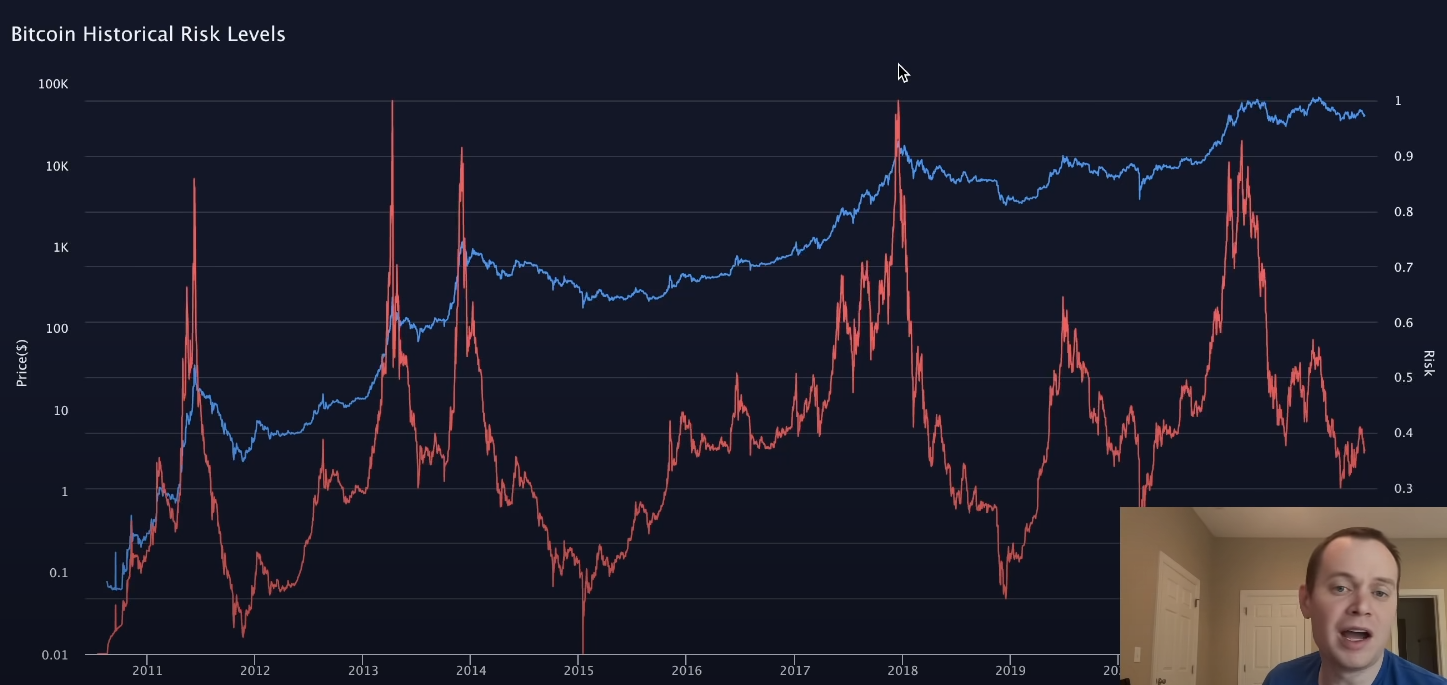
\includegraphics[width=\columnwidth]{figures/cowen-riskmetric-screenshot.png}
    \caption{Screenshot of Benjamin Cowen's Bitcoin risk metric from video~\cite{youtube:bitcoin-risk-metric-latest}. Attribution: Benjamin Cowen~\cite{youtube:cowen-yt-channel}.}
    \label{figure-cowen-screenshot}
\end{figure}

\begin{figure}[!t]
    \centering
    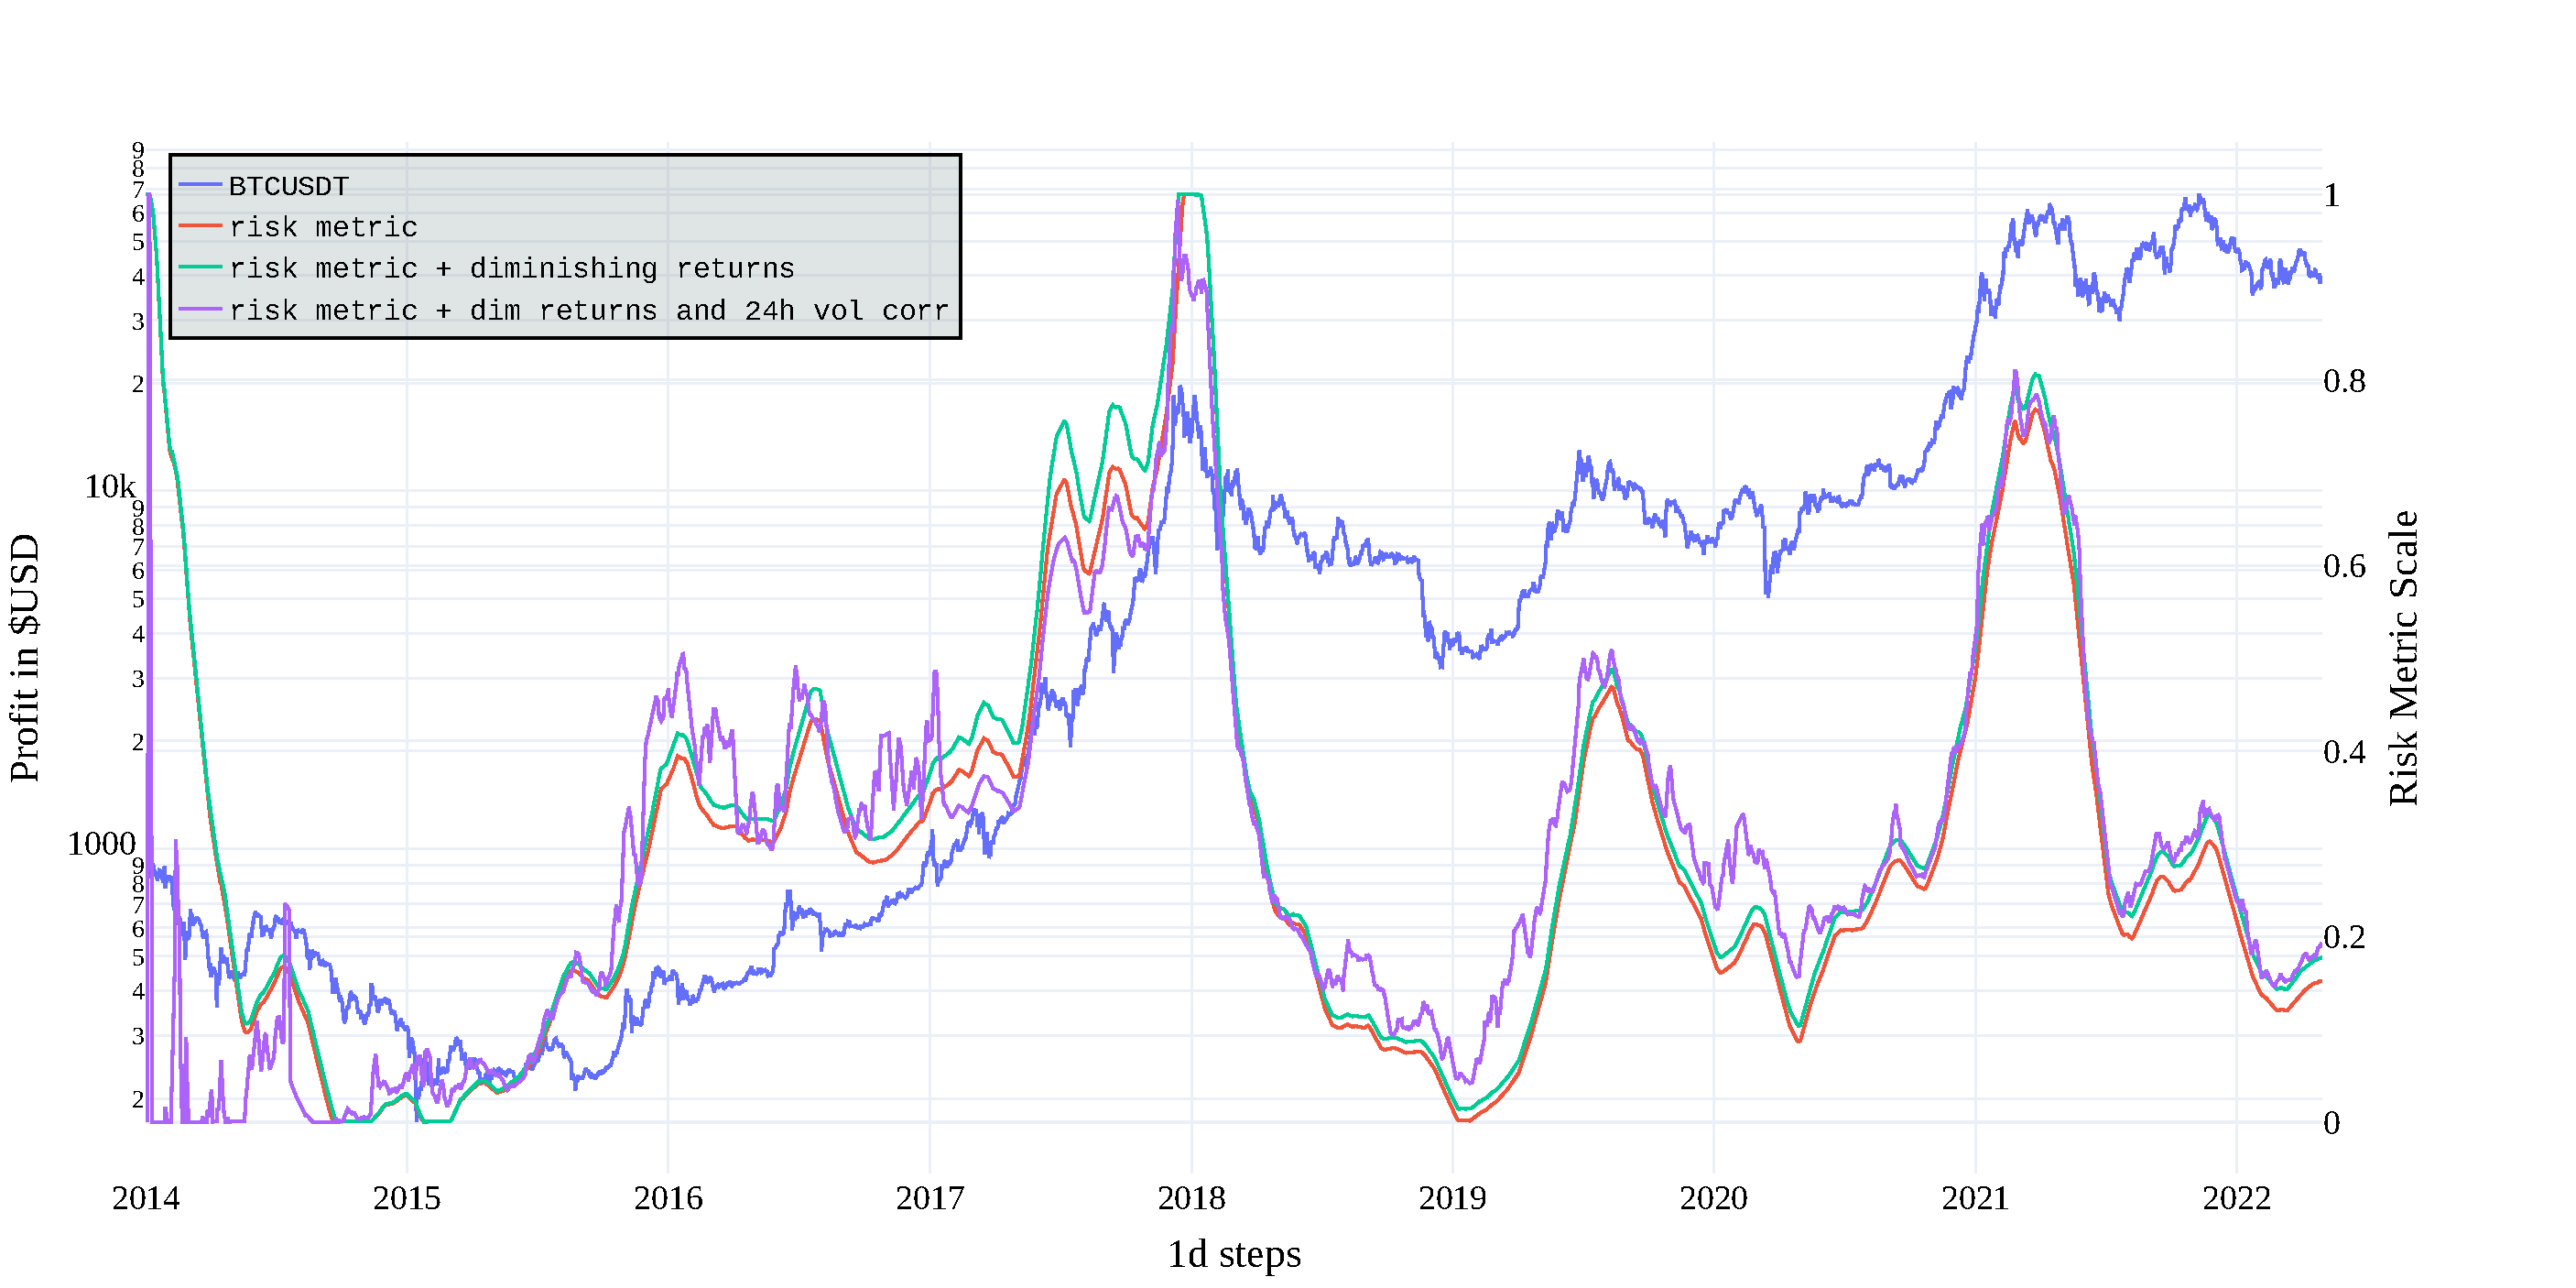
\includegraphics[width=\columnwidth]{figures/combined-bitcoin-metrics.pdf}
    \caption{Showcase of the thesis's Bitcoin risk metrics.}
    \label{figure-combined-bitcoin-riskmetric}
\end{figure}

\subsection*{Comparing My Strategies To Automated Bot Systems}
Looking at automated bot systems, two working commercial bot systems have been analyzed, Pionex~\cite{pionex} and 3Commas~\cite{3commas}. Since I~do not have any account with either of them, the offered features are analyzed instead. Pionex uses an interesting feature called Grid trading~\cite{pionex-grid-trading}, it uses a set grid of prices that are used to capitalize the market's fluctuations. Capitalizing the market's fluctuations is the topic of the Section~\ref{section-testing-day-trading}, where a bit different approach is used. Other Pionex's bots include DCA bot and rebalance bot. Both of these bots are easily backtested with the thesis backtester framework.

3Commas offers options to backtest your own strategy within their framework~\cite{3commas-trading-view}. I~would guess that backtesting in such a way is easier for investors not skilled in programming. It offers similar features as Pionex, including the DCA and HODL bots.


\section{Further Ideas and Involvement}
The science and technical analysis of cryptocurrencies is a vast subject and time is limited. There is an infinite number of things to test and analyze. The framework itself could be improved. Below are some strategies, optimizations and ideas that I~considered during the thesis and that can be worked on in further involvement.

\subsection*{Strategies}
Top 7 trading cryptocurrencies CoinGecko API endpoint~\cite{coingecko:documentation} could be used to buy trending cryptocurrencies based on the belief that they will rise soon.

It would be advisable to add trending strategies to a portfolio dynamically during the run, rather than starting with the top 20 portfolio only. Some interesting results may be found if we change the coins dynamically, selling those that underperform periodically and add the ones that got bigger capitalization recently.

Strategy correlation with FIAT money inflation would be interesting to see. The argument there is that as people have more money, the price naturally rises to match it.

More intensive research regarding machine learning, and its correlation to other findings, would definitely be interesting.

One interesting strategy would be to find the risk metric for every coin in the portfolio and measure the risks and investments individually on a per-coin basis.

Stablecoin trading would be a good strategy to generate profit during longer bear markets. This would mean that the strategy is always looking for an opportunity to generate money, even if the market is not hospitable. This would make the whole strategy process even more resilient to the market changes.

\subsection*{Backtester Optimization}
Saving already computed strategies to the filesystem could be implemented to severely help save the time between individual runs of similar strategies. For example, the HODL strategy that the more interesting strategies are benchmarked against is the same between each individual run, same with rebalance.

A~possible web application could be built to better the user experience with the tool itself. Graphs would be generated on-site with possible configuration switches and sliders.

The configuration file could be extended to include strategy definitions too. With this approach no tampering with code would be needed and all the runtime backtesting would be defined by the configuration file only. This approach has not been chosen for the thesis because of the ever-changing implementation in an iterative way.

\subsection*{Better Profit Analysis}
P\&L per trade visualization could be informative, as well as incorporating other metrics like the Sharpe Ratio into the statistics output.

\chapter{Conclusion}
\label{conclusion}
The goal of the thesis was to propose and implement adaptive trading strategies that would adapt to the rising and falling markets and generate more stable profits. The goal has been achieved and demonstrated in several ways, focusing on both long-term and short-term date ranges. In the process, an extensible backtesting framework was created, general enough to support the implementation of both long-term and short-term strategies.

Regarding the thesis formal specification. Existing trading strategies were studied and achieved results analyzed and assumptions summarized. Existing simulation tools were described. Cryptocurrency trading data was analyzed and events of interests were summarized. Adaptive trading strategies were proposed, implemented in the form of a backtester and evaluated against traditional approaches. Both 5 minute OHLCV and 1 day OHLCV data were used during the thesis. Finally, further improvements and limitations of the practical deployment were described.

It was found that the Bitcoin risk metric, can be used as a form of adaptive trading strategy for long-term investing. It was shown how different approaches can optimize such metrics, such as using the total market capitalization price instead of Bitcoin price, or correlating the metric with the daily traded volume, can lead to better results under certain conditions. Regarding the short-term strategy, buying and selling at local extrema of price's smooth moving average was explored. All strategy results were compared to traditional approaches like HODL and rebalance. Under the right criteria, the performance was multiplied several times.

I~learned in great detail about economics of the market trading and cryptocurrencies in general. I~understand how a backtester can be built now and how should a trading strategy be implemented.

Regarding my future plans, I~plan to keep working on the backtester itself. There are several improvements that could be applied, such as optimizing the backtester's computing time, or creating a web user interface. There are many strategies that should be explored too, for example, trying to generate profit from trading stablecoins when holding them, exploring machine learning in a greater detail, and many others. More advanced profit analysis, such as Sharpe Ratio, and P\&L per trade visualization, may lead to interesting discoveries. My other plans are to make an automated trading system that would use the strategies backtested by the backtester program.


  % Kompilace po částech (viz výše, nutno odkomentovat)
  % Compilation piecewise (see above, it is necessary to uncomment it)
  %\subfile{projekt-01-uvod-introduction}
  % ...
  %\subfile{chapters/projekt-05-conclusion}


  % Pouzita literatura / Bibliography
  % ----------------------------------------------
\ifslovak
  \makeatletter
  \def\@openbib@code{\addcontentsline{toc}{chapter}{Literatúra}}
  \makeatother
  \bibliographystyle{bib-styles/Pysny/skplain}
\else
  \ifczech
    \makeatletter
    \def\@openbib@code{\addcontentsline{toc}{chapter}{Literatura}}
    \makeatother
    \bibliographystyle{bib-styles/Pysny/czplain}
  \else
    \makeatletter
    \def\@openbib@code{\addcontentsline{toc}{chapter}{Bibliography}}
    \makeatother
    \bibliographystyle{bib-styles/Pysny/enplain}
  %  \bibliographystyle{alpha}
  \fi
\fi
  \begin{flushleft}
  \bibliography{xfilip46-thesis-20-bibliography}
  \end{flushleft}

  % vynechani stranky v oboustrannem rezimu
  % Skip the page in the two-sided mode
  \iftwoside
    \cleardoublepage
  \fi

  % Prilohy / Appendices
  % ---------------------------------------------
  \appendix
\ifczech
  \renewcommand{\appendixpagename}{Přílohy}
  \renewcommand{\appendixtocname}{Přílohy}
  \renewcommand{\appendixname}{Příloha}
\fi
\ifslovak
  \renewcommand{\appendixpagename}{Prílohy}
  \renewcommand{\appendixtocname}{Prílohy}
  \renewcommand{\appendixname}{Príloha}
\fi
%  \appendixpage

% vynechani stranky v oboustrannem rezimu
% Skip the page in the two-sided mode
%\iftwoside
%  \cleardoublepage
%\fi

\ifslovak
%  \section*{Zoznam príloh}
%  \addcontentsline{toc}{section}{Zoznam príloh}
\else
  \ifczech
%    \section*{Seznam příloh}
%    \addcontentsline{toc}{section}{Seznam příloh}
  \else
%    \section*{List of Appendices}
%    \addcontentsline{toc}{section}{List of Appendices}
  \fi
\fi
  \startcontents[chapters]
  \setlength{\parskip}{0pt}
  % seznam příloh / list of appendices
  % \printcontents[chapters]{l}{0}{\setcounter{tocdepth}{2}}

  \ifODSAZ
    \setlength{\parskip}{0.5\bigskipamount}
  \else
    \setlength{\parskip}{0pt}
  \fi

  % vynechani stranky v oboustrannem rezimu
  \iftwoside
    \cleardoublepage
  \fi

  % Přílohy / Appendices
  % Author: Marek Filip 2022

% This file should be replaced with your file with an appendices (headings below are examples only)

% Placing of table of contents of the memory media here should be consulted with a supervisor

\chapter{Contents of the included storage media}
\begin{verbatim}
.
├── .flake8
├── args.yaml
├── docker-compose.yml
├── Dockerfile
├── LICENSE
├── Makefile
├── README.md
├── pyproject.toml
├── requirements-lint.txt
├── requirements.txt
├── requirements-freeze.txt (Dependcies with specified versions.)
├── text (Thesis Latex folder.)
├── tests (Backtester test files.)
├── backtester (Backtester source codes.)
├── data (Sample data so that Binance API is not needed)
└── xfilip46-thesis.pdf (Thesis text output.)
\end{verbatim}


\chapter{Manual}
Usage is defined in the standard environment of bash command line interface. All needed commands are provided by the Makefile and can be listed by running \texttt{make}.

\subsection*{Installation}
Multiple options are available for installation. Python version 3.9 should be installed on the target system.

Local install:
\begin{minted}{bash}
make installdeps
\end{minted}

Virtual environment installation:
\begin{minted}{bash}
make create-venv
. venv/bin/activate
make installdeps
\end{minted}

Containerized development:
\begin{minted}{bash}
make docker-build  # docker-compose build
\end{minted}

\subsection*{How to Run the Project}
There are a few ways to run the project.

Via Makefile:
\begin{minted}{bash}
make run
\end{minted}

With arguments:
\begin{minted}{bash}
python -m backtester <your_arguments>
\end{minted}

Via Docker:
\begin{minted}{bash}
make docker-up  # docker-compose up
\end{minted}

The \texttt{args.yaml} configuration file should be edited to change the backtester behaviour. After that, the \texttt{simulate()} function found in the file \texttt{simulator.py} can be edited to make other strategies and plotting available.

\subsection*{How to Develop New Strategies}
To create new strategies, you can create any valid Python file and import the \texttt{Strategy} base class defined in strategy.py.
You can then include the created strategy inside the \texttt{simulator.py} file, where you can also define what shoudl the Plotter class plot.
There are several showcase functions inside the \texttt{simulate()} function for new devoleprs to play around with.
Finally, changing \texttt{args.yaml} may be necessarry to adjust the input variables if you plan on running the program by \texttt{make run}.


  % Kompilace po částech (viz výše, nutno odkomentovat)
  % Compilation piecewise (see above, it is necessary to uncomment it)
  %\subfile{xfilip46-thesis-30-prilohy-appendices}

\end{document}
